\chapter{Self-Supervised Representation Learning for Wireless Signals}
\label{chap:background}

\section{Introduction}

Foundation models in computer vision demonstrate that self-supervised pre-training on large unlabeled datasets produces representations transferable across diverse downstream tasks with minimal fine-tuning. Vision Transformers (ViT) pre-trained via masked autoencoding~\cite{he2022masked} achieve remarkable performance on image classification, object detection, and segmentation despite never seeing task-specific labels during pre-training. This chapter establishes analogous principles for wireless signals, asking: \textit{Can we learn universal representations from unlabeled wireless data that transfer across modulation schemes, noise conditions, and communication tasks?}

We present three complementary contributions that progressively build toward this goal:

\textbf{NMformer} adapts Vision Transformers to wireless modulation classification using constellation diagrams as visual representations of wireless signals. By treating constellation images as patch sequences and applying self-attention, NMformer learns global signal structure robust to noise. This work establishes that transformer architectures—cornerstone of modern foundation models—are viable for wireless signal processing, achieving high accuracy across SNR ranges with minimal fine-tuning.

\textbf{DenoMAE} introduces multimodal masked autoencoders specifically designed for wireless signals. Unlike vision MAE which masks image patches, DenoMAE jointly masks and reconstructs across two modalities: time-domain IQ samples and constellation diagrams. Crucially, we treat noise as an explicit modality to model rather than mere corruption to overcome. By learning to reconstruct both signal content and noise characteristics, DenoMAE discovers representations capturing fundamental wireless signal properties independent of specific modulation types. The learned encodings transfer effectively to downstream classification with dramatically reduced labeled data requirements.

\textbf{DenoMAE 2.0} extends the masked autoencoding framework by combining global reconstruction with local discriminative objectives. While DenoMAE focuses on holistic signal reconstruction, DenoMAE 2.0 adds auxiliary patch-level classification, forcing the model to learn both coarse-grained global structure and fine-grained local patterns. This hybrid generative-discriminative approach yields representations particularly effective in low-SNR regimes where local features become crucial for disambiguation.

These three methods collectively demonstrate that wireless signals—despite lacking explicit semantic content—can be represented through learned embeddings that capture transferable properties. The representations learned by DenoMAE become the foundation for later chapters: they enable few-shot meta-learning (Chapter 3), support efficient semi-supervised training (Chapter 4), and critically, serve as semantic features for language model integration (Chapter 5). This chapter thus establishes the representation learning foundation upon which our wireless foundation model framework is built.

Our contributions advance wireless signal processing on multiple fronts: architecturally, by adapting transformers and masked autoencoders to wireless domains; methodologically, by treating noise as informative modality and multimodal signals jointly; and conceptually, by demonstrating that self-supervised pre-training principles from vision transfer to wireless with appropriate domain adaptation. Through extensive experiments on standard benchmarks (RadioML datasets), we validate that these approaches achieve state-of-the-art performance while learning representations that generalize beyond their training distribution—a key requirement for foundation models.

\section{Automatic Modulation Classification: Foundation Model Perspective}

Automatic Modulation Classification (AMC) serves as an ideal testbed for developing wireless foundation models. AMC requires understanding fundamental signal properties (constellation structure, symbol timing, spectral characteristics) that transfer across communication scenarios. Unlike end-to-end communication system design, AMC focuses on recognizing signal types—a task analogous to image classification in vision, making it well-suited for foundation model approaches.

In today’s increasingly connected world, wireless communication has become the foundation of modern life. From smartphones and Wi-Fi to satellite systems and military radios, the seamless exchange of data over the airwaves is a remarkable technological achievement. A crucial but often overlooked part of this process is understanding how information is encoded onto signals — a task that becomes particularly important when the modulation scheme of a signal is unknown or rapidly changing. This is where Automatic Modulation Classification (AMC) comes into play~\cite{azzouz1996automatic}.

At its core, AMC is the process by which a wireless receiver determines the modulation type of a received signal without prior knowledge. Modulation is the technique used to encode data onto a carrier wave — altering its amplitude, frequency, or phase to represent digital or analog information. The ability to automatically identify this modulation is essential in many non-cooperative or dynamic communication scenarios, where the receiver has limited information about the signal’s origin or format~\cite{swami2000hierarchical}.

In traditional communication systems, the transmitter and receiver are designed to operate with a shared set of parameters, including the modulation scheme. However, this assumption does not hold in many real-world applications. For instance, in military or surveillance contexts, a system might intercept signals from unknown sources. Similarly, cognitive radios — smart devices that dynamically access available spectrum — must identify and adapt to the modulation schemes of nearby transmissions to avoid interference~\cite{yucek2009survey}. In these cases, AMC enables the receiver to make sense of unfamiliar signals quickly and reliably.

AMC also plays a vital role in spectrum monitoring and management. As more devices compete for limited wireless bandwidth, understanding how that spectrum is being used becomes increasingly important. Regulators and service providers use AMC to analyze traffic patterns, detect anomalies, and ensure fair usage across frequency bands. Moreover, as networks grow more heterogeneous, incorporating different types of devices and standards, AMC helps maintain interoperability by allowing systems to adapt to each other's communication styles.

Despite its benefits, implementing AMC is not without challenges. Wireless environments are notoriously unpredictable — signals often encounter noise, fading, reflections, and other distortions as they travel. This makes it harder for a receiver to accurately identify the modulation, especially under low signal-to-noise conditions~\cite{gardner1994cyclostationarity}. Additionally, real-time classification requires systems that are both fast and resource-efficient, which can be a constraint for mobile or embedded devices.

Nonetheless, advances in signal processing and artificial intelligence have significantly improved the performance and reliability of AMC systems. With the rise of machine learning, particularly deep learning, modern AMC frameworks are becoming more robust to environmental variations and capable of handling a wider range of signal types~\cite{rajendran2018deep, oshea2016convolutional}. These developments are pushing the boundaries of what’s possible in adaptive and intelligent communication systems.

% TODO: Add a figure of the AMC process

\section{Automatic Modulation Classification: Foundation Model Perspective}

Automatic Modulation Classification (AMC) serves as an ideal testbed for developing wireless foundation models. AMC requires understanding fundamental signal properties (constellation structure, symbol timing, spectral characteristics) that transfer across communication scenarios. Unlike end-to-end communication system design, AMC focuses on recognizing signal types—a task analogous to image classification in vision, making it well-suited for foundation model approaches.

At its core, AMC determines the modulation type of a received signal without prior knowledge~\cite{azzouz1996automatic}. Modulation encodes information onto carrier waves by varying amplitude, frequency, or phase. Traditional communication assumes transmitter and receiver share modulation parameters. However, many scenarios violate this assumption: military surveillance intercepts unknown signals, cognitive radios must identify neighboring transmissions to avoid interference~\cite{yucek2009survey}, and spectrum monitoring systems analyze heterogeneous traffic patterns.

The challenge of AMC mirrors challenges facing foundation models generally: the input space is vast (countless modulation schemes, varying SNRs, diverse channel conditions), labeled data is expensive (especially for rare or proprietary schemes), and systems must generalize to distribution shifts (new modulation types, hardware impairments, adversarial signals). Current AMC systems are brittle, trained on fixed modulation sets and failing catastrophically on novel signals. This motivates our foundation model approach: learn universal representations of wireless signals that enable zero-shot or few-shot recognition of new modulation types.

\subsection{From Closed-Set to Open-Set Recognition}

Traditional AMC frames the problem as closed-set classification: given signal $x$, predict one of $K$ known modulation types. This assumption is fundamentally limiting. Real wireless systems encounter:

\begin{itemize}
    \item \textbf{Novel Modulations:} New communication standards introduce modulation schemes not in training data
    \item \textbf{Hybrid Schemes:} Adaptive modulation systems switch between types based on channel conditions
    \item \textbf{Adversarial Signals:} Intentional interference or spoofing with non-standard modulations
    \item \textbf{Hardware Variations:} Implementation differences create signal variations within nominal modulation types
\end{itemize}

Foundation models address this through open-set recognition: the system should detect when it encounters something truly novel rather than forcing every input into known categories. Our approach using DenoMAE encodings for LLM-based reasoning (Chapter 5) enables this capability—the model can describe signal properties it observes and reason about whether they match known modulation descriptions, even for schemes never seen during training.

\subsection{The Role of AMC in Wireless Foundation Models}

While this dissertation uses AMC as the primary application, the principles extend to broader wireless AI:

\begin{itemize}
    \item \textbf{Channel Estimation:} Learned signal representations could enable estimation of channel parameters from received signals
    \item \textbf{Signal Denoising:} The denoising capability of DenoMAE transfers to general noise reduction tasks
    \item \textbf{Spectrum Sensing:} Detecting presence and characteristics of signals in spectrum monitoring
    \item \textbf{Physical Layer Security:} Identifying anomalous or adversarial transmissions
    \item \textbf{Cross-Layer Optimization:} Representations enabling joint optimization of physical and higher layers
\end{itemize}

AMC provides a well-defined, experimentally tractable problem for developing and validating foundation model approaches. Success in AMC—learning representations that transfer across modulation schemes and enable open-set recognition—suggests viability for broader wireless AI applications. The remainder of this chapter focuses on representation learning techniques specifically designed to capture universal wireless signal properties.

\section{Background: Traditional AMC to Foundation Model Era}

The evolution of automatic modulation classification mirrors the broader trajectory of machine learning: from handcrafted features to learned representations, from supervised to self-supervised learning, and from closed-set to open-set recognition. Understanding this progression contextualizes our contributions and highlights how foundation model thinking transforms wireless signal processing.

The field of automatic modulation classification has evolved significantly over the past decades, transitioning from traditional statistical methods to sophisticated machine learning approaches. This section examines this progression through the lens of foundation model development: understanding what previous approaches lacked and what modern self-supervised methods provide. We trace the evolution from handcrafted features to learned representations, from supervised to self-supervised learning, and from closed-set to open-set recognition—each transition bringing us closer to wireless foundation models.

\subsection{Traditional Modulation Classification Approaches}\label{sec:traditional}

Early research in AMC predominantly focused on two main paradigms: likelihood-based (LB) methods, which aim for statistical optimality, and feature-based (FB) methods, which prioritize computational simplicity and practicality by extracting discriminative signal characteristics.

\paragraph{Likelihood-Based (LB) Approaches.}

Early automatic modulation classification (AMC) systems formulated the modulation recognition problem as multiple-hypothesis testing, selecting the modulation scheme that maximizes the likelihood of observed baseband samples \cite{wei2000, dobre2007}. The maximum-likelihood classifier (MLC) achieves Bayes-optimal performance when complete signal and channel parameters are known \cite{wei2000}. To address practical scenarios with unknown parameters, researchers developed variants including average (ALRT), generalized (GLRT), and hybrid likelihood-ratio tests that estimate unknown parameters through marginalization or plug-in estimates \cite{dobre2007}.

Despite their theoretical elegance, likelihood-based methods face significant implementation challenges in real-time radio systems. These limitations include: (1) combinatorial complexity when searching across unknown phase, timing, noise variance, and symbol sequences; (2) dependency on accurate channel statistics; and (3) substantial performance degradation under model mismatch or non-Gaussian interference conditions.

\paragraph{Feature-based (FB) approaches.}

Feature-based (FB) approaches aim to reduce the complexity of likelihood-based (LB) methods by extracting low-dimensional, discriminative statistics, which are then classified using techniques such as thresholding, decision trees, or support vector machines (SVMs). Among these, higher-order cumulants are widely utilized; notably, the hierarchical fourth-order cumulant classifier developed by Swami and Sadler remains a benchmark, offering robust performance in low signal-to-noise ratio (SNR) environments due to the property that all higher-order cumulants of Gaussian noise vanish~\cite{swami2000hierarchical}. Cyclostationary statistics exploit periodic correlations introduced by the symbol rate or carrier frequency and are resilient to unknown timing and phase offsets~\cite{gardner1994}.

Other handcrafted descriptors, such as instantaneous amplitude/phase, wavelet-domain features, and constellation density metrics, have been proposed \cite{6487244, al2019performance}. However, FB methods are considered sub-optimal because the manual feature extraction process can discard useful information, is sensitive to channel variations, and often requires re-engineering for each new air-interface.

\textbf{Foundation Model Gap:} Both likelihood-based and feature-based methods share a fundamental limitation: they require explicit modeling or feature engineering by domain experts. They cannot learn transferable representations from data itself. Each new modulation scheme or channel condition requires manual re-design. This brittleness motivated the shift to deep learning.

\subsection{Deep Learning for Modulation Classification}

The shortcomings of LB and FB methods, including their heavy computational overhead and fragile hand-crafted feature pipelines, motivated the adoption of deep learning (DL) approaches for AMC. By directly learning hierarchical representations from minimally processed baseband signals (e.g., IQ samples), DL methods aim to overcome the bottlenecks inherent in LB and FB paradigms.

Early DL research was dominated by convolutional neural networks (CNNs).  O'Shea and Corgan showed that a shallow CNN fed with raw IQ vectors or constellation-image tensors can outperform classical FB techniques, especially at low SNR \cite{o2016convolutional}.  Follow-up work deepened these architectures—adding residual connections or squeeze-excitation blocks—to create more expressive yet still convolutional models \cite{8963964}.  To capture temporal dynamics that CNNs may miss, \emph{recurrent} models such as LSTM- or GRU-based classifiers were explored, either standalone or in hybrid CNN-RNN stacks; sequential processing improved recognition of long-range dependencies and yielded further accuracy gains \cite{10505944}.  

Despite the performance gains delivered by deep architectures, DL‑based AMC still encounters three recurring obstacles: vanishing or unstable gradients that hamper the optimisation of very deep networks on long IQ sequences, prompting the use of residual and sequence‑gated remedies~\cite{liao2021sequential}; chronic data scarcity, since assembling large, labelled waveform corpora across diverse channels is costly, leading researchers to rely on aggressive augmentation, synthetic data generation, and transfer‑learning pipelines to exploit unlabeled signals~\cite{bu2020adversarial,zheng2021spectrum}; and stringent edge‑deployment constraints, because state‑of‑the‑art models often exceed the latency, memory, and power budgets of IoT or UAV radios, motivating lightweight architectures that prune parameters, quantise weights, or embed efficient attention blocks while preserving accuracy~\cite{wang2023automatic}.

\textbf{Foundation Model Gap:} While deep learning learns representations from data, supervised CNNs and RNNs remain task-specific. They learn discriminative features for a fixed set of modulation types but fail to generalize to unseen schemes. The representations are tightly coupled to the classification objective rather than capturing universal signal properties. This motivated self-supervised and transformer-based approaches.

\subsection{Recent Advances in Wireless Communication}\label{sec:recent}

Driven by the growing complexity of wireless environments, recent work has adapted more expressive neural architectures—originally devised for natural–language and vision tasks—to automatic modulation classification (AMC).  Transformers were first ported to raw IQ sequences after their success in natural‑language processing; the self‑attention mechanism captures long‑range dependencies that elude local convolutions, yielding sizeable gains at low SNR \cite{vaswani2017attention,damasevicius2024tfi}. Vision Transformers (ViT) extend this idea to two‑dimensional signal representations: constellation diagrams and spectrograms are treated as patch sequences so that global spatial structure can be modelled via attention, improving robustness to noise‑induced distortion \cite{dosovitskiy2021vit,shao2024iqformer}.  In parallel, Graph Neural Networks (GNNs) have been explored for AMC by casting samples or spectral components as graph nodes and learning over their relational topology, an approach shown to enhance classification under multi‑path interference and cross‑modality fusion settings \cite{liu2020gcn,marwani2024graph}.

Recognising the complementary inductive biases of different backbones, researchers have proposed hybrid designs that combine CNNs for local feature extraction with Transformers or RNNs for global or temporal reasoning, and even GNN layers for relational aggregation \cite{damasevicius2024tfi,chen2024survey}.  Such composites aim to exploit spatial, sequential and structural cues simultaneously, delivering state‑of‑the‑art accuracy across diverse channel conditions.

Alongside the push for accuracy, a parallel line of inquiry targets lightweight AMC suitable for edge deployment.  Techniques range from depth‑wise separable convolutions and efficient attention blocks to parameter pruning, weight quantisation and knowledge distillation; custom networks such as MobileRaT, MobileAmcT and other mobile‑ViT variants demonstrate that meaningful reductions in FLOPs and model size can be achieved with minimal loss in accuracy \cite{xuan2022avgnet,zheng2023mobilerat,fei2024mobileamct}.  Balancing these resource constraints with classification performance remains a central challenge for real‑time, on‑device AMC.

\textbf{Foundation Model Alignment:} Transformers and attention mechanisms represent crucial architectural advances toward foundation models. Their ability to model global dependencies and process multimodal inputs (constellation diagrams, spectrograms) provides the architectural foundation. However, most work still trains these architectures in supervised closed-set settings. Our NMformer contribution (Section~\ref{sec:nmformer}) demonstrates Vision Transformers for wireless signals, while DenoMAE (Section~\ref{sec:denomae}) introduces self-supervised pre-training—the missing piece for true foundation models.

\section{Self-Supervised and Semi-Supervised Learning for Wireless Signals}

As purely supervised approaches face persistent challenges due to the scarcity and cost of labeled wireless-signal datasets, self-supervised and semi-supervised learning strategies have gained prominence in automatic modulation classification (AMC). These methods represent crucial steps toward foundation models: they learn from unlabeled data to discover representations that transfer across tasks. This section reviews key paradigms—contrastive learning, representation learning, and masked reconstruction—that inform our DenoMAE framework.

\subsection{Contrastive Learning}

\textbf{Contrastive learning} has recently emerged as promising solutions to the pervasive scarcity of labeled data in automatic modulation classification (AMC). Inspired by advances such as SimCLR \cite{chen2020simclr} and MoCo \cite{he2020moco} from computer vision, contrastive methods create supervisory signals by pulling representations of augmented views from the same input closer while pushing apart representations of different instances \cite{bu2020adversarial}. When adapting this strategy to AMC, augmentations typically involve signal perturbations like noise addition, frequency shifts, phase offsets, or time-segment shuffling, thus encouraging learned representations to remain invariant to common wireless-channel variations \cite{zheng2021spectrum}. While these methods effectively leverage unlabeled data, their success strongly depends on carefully designed augmentation policies and informative negative-sample selection, posing particular challenges in highly noisy wireless environments \cite{bu2020adversarial, zheng2021spectrum}.

\textbf{Limitations for Foundation Models:} Contrastive methods require large batch sizes (SimCLR needs 4096+ samples) and carefully engineered augmentations. For wireless signals, defining "positive pairs" is non-trivial—which augmentations preserve signal identity versus changing modulation properties? Moreover, contrastive learning focuses on instance discrimination rather than learning to reconstruct signal structure, limiting its effectiveness for tasks beyond classification.

\subsection{Representation Learning via Autoencoders}

\subsection{Representation Learning via Autoencoders}

Representation learning approaches, particularly autoencoders (AEs) and variational autoencoders (VAEs), provide another pathway by focusing on learning robust latent representations of signal data. AEs achieve this through reconstruction objectives, compressing input signals into bottleneck latent codes, whereas VAEs introduce probabilistic constraints on the latent space to encourage structured and noise-resistant representations \cite{kingma2014vae}. Applied within AMC, these models typically serve dual purposes: extracting compressed signal representations useful for downstream classification, and performing implicit signal denoising by reconstructing clean waveforms from noisy inputs \cite{an2015variational,jiang2019semi}. Nevertheless, standard AE and VAE objectives prioritize reconstruction rather than class separability, potentially limiting their discriminative power for modulation classification tasks \cite{an2015variational}.

A more recent approach in representation learning is learning two variants of the same representation, through augmentation or distortion to the inputs. This strategy eliminates the need for negative samples and make the learning process faster and more effective. The two representations are then compared using a consistency loss function, which encourages the model to learn meaningful features that are invariant to the augmentations applied. This approach has shown promise in various domains, including image classification and natural language processing, and is now being explored in the context of AMC~\cite{10034661}. Non-contrastive methods like BYOL \cite{grill2020bootstrap} and SimSiam~\cite{chen2020exploring} avoid the need for explicit negative pairs, using architectural or operational asymmetries (e.g., momentum encoders, stop-gradients) to prevent representational collapse. Barlow Twins \cite{zbontar2021barlow} offers another approach, focusing on reducing redundancy within the learned feature vectors.

A critical challenge across all SSL methods when applied to AMC is the design of effective, signal-specific data augmentations – transformations that alter the signal without destroying its core modulation identity \cite{wang2024semi}. Unlike image data where standard augmentations are well-established, finding equivalent transformations for complex-valued time-series signals requires domain expertise and is an active area of research \cite{islam2024systematic}. Despite this challenge, SSL holds significant promise for enhancing AMC by learning robust, discriminative features from abundant unlabeled wireless data \cite{wu2022deep}.

\textbf{Path to Foundation Models:} Autoencoder-based representation learning provides the foundation for our DenoMAE approach. However, standard autoencoders learn representations optimized for reconstruction, not necessarily capturing modulation-specific or transferable features. Masked autoencoders (next section) address this by learning to predict missing content, forcing the model to understand signal structure rather than memorizing superficial patterns.

\subsection{Masked Autoencoders for Wireless Signals}

\subsection{Masked Autoencoders for Wireless Signals}

\textbf{Masking strategies} have increasingly become integral within self-supervised learning frameworks, driven by the notable success of masked autoencoder (MAE)-based techniques originally developed for computer vision (MAE~\cite{he2022mae}) and natural-language processing (BERT~\cite{vaswani2017attention}). The core insight is simple yet powerful: by masking portions of the input and learning to reconstruct them, models must develop deep understanding of the underlying structure rather than memorizing surface patterns.

Masking methods deliberately obscure portions of input signals, tasking neural encoders and lightweight decoders with reconstructing missing segments, thereby implicitly learning robust contextual dependencies within the data \cite{he2022mae}. For AMC specifically, these strategies have been adapted across diverse signal domains. Niizumi et~al. \cite{niizumi2022masked} applied spectrogram masking techniques that obscure frequency-time regions, forcing the model to learn spectral relationships that persist even when portions of the signal are corrupted. Medhat et~al.~\cite{medhat2020masked} extend these ideas to frequency-domain features, demonstrating that masking strategies can be effective across different signal representations. These approaches share conceptual similarities with BERT in natural language processing and MAE in computer vision, adapting self-supervised pretraining paradigms to wireless communication challenges.

Extensions incorporating auxiliary classification tasks during masking-based pre-training further refine learned representations, enhancing discriminability and effectively balancing global reconstruction objectives with local modulation-specific features \cite{he2022mae}. This hybrid approach—combining generative reconstruction with discriminative classification—motivates our DenoMAE 2.0 contribution where local patch classification augments global masked reconstruction.

\textbf{Foundation Model Connection:} Masked autoencoders represent the most promising path to wireless foundation models. Unlike contrastive learning's dependence on augmentations or supervised learning's need for labels, masked reconstruction learns directly from signal structure. MAE's success in vision (enabling models like ViT to achieve strong performance with less data) suggests analogous potential for wireless signals. Our DenoMAE framework (Section~\ref{sec:denomae}) extends MAE principles to multimodal wireless signals with explicit noise modeling—a key innovation for wireless foundation models.

\subsection{Multimodal Learning Based Methods}\label{sec:multi}

Multimodal representation learning seeks to build models that integrate information from diverse sources, such as vision, language, audio, and sensor data like radio frequency (RF) signals \cite{yuan2025survey}, aiming for a more comprehensive understanding than unimodal approaches. The core motivation lies in leveraging complementary information across modalities  to enhance model accuracy, robustness, particularly in noisy or data-scarce scenarios \cite{akkus2023multimodal}, and transferability. Key objectives involve bridging the 'heterogeneity gap'  by learning joint or coordinated representations \cite{li2024multimodal}, enabling cross-modal translation, and facilitating effective fusion for downstream tasks. Common strategies range from simple feature concatenation or element-wise operations to sophisticated attention mechanisms, notably cross-modal attention within transformer architectures, which implicitly learn alignments and interactions \cite{liang2024crossformer}. A dominant paradigm involves learning joint embedding spaces, often via contrastive objectives applied to large-scale paired datasets. Works like CLIP \cite{radford2021learning} and ALIGN \cite{jia2021scaling} demonstrated that training image and text encoders contrastively on web-scale data yields powerful, transferable representations capable of impressive zero-shot generalization, highlighting the efficacy of natural language supervision.

These principles find application in specialized domains such as signal processing, particularly for Automatic Modulation Classification (AMC), which aims to identify the modulation scheme of received signals \cite{qiu2023deepsig}. Multimodal AMC leverages diverse signal representations—including raw I/Q sequences, constellation diagrams, time-frequency distributions, or spectral correlation functions \cite{xu2025mclrl}—to improve classification accuracy, especially in low signal-to-noise ratio (SNR) conditions where traditional methods falter \cite{li2022amcmlp}. Specific frameworks adapt general techniques: DeepSIG employs hybrid architectures for heterogeneous signal inputs \cite{qiu2023deepsig}, MCLRL combines multi-domain contrastive learning with reinforcement learning for few-shot AMC \cite{xu2025mclrl} uses a multimodal autoencoder for improving data efficiency. While offering benefits like improved performance and robustness, multimodal learning faces challenges including increased model complexity, effective alignment and fusion across heterogeneous data types, handling missing modalities \cite{wu2024deep}, and mitigating modality dominance or imbalance \cite{haouhat2023modality}. Efficient adaptation of large pre-trained models using techniques like MMLoRA \cite{wang2023improving, sun2024improving} and generative approaches like MVAE \cite{wu2018multimodal} or SMVAE \cite{zhou2022generalizing, zhou2022span} for modeling joint distributions and handling missing data represent ongoing research directions addressing these practical hurdles.

\subsection{Multimodal Learning Based Methods}\label{sec:multi}

Multimodal representation learning seeks to build models that integrate information from diverse sources, aiming for more comprehensive understanding than unimodal approaches. For wireless signals, this means jointly processing time-domain IQ samples, constellation diagrams, spectrograms, and potentially other representations \cite{yuan2025survey}. The core motivation lies in leveraging complementary information across modalities to enhance model accuracy, robustness, particularly in noisy or data-scarce scenarios \cite{akkus2023multimodal}, and transferability.

The success of multimodal foundation models like CLIP \cite{radford2021learning}—which learns joint vision-language representations enabling zero-shot classification—demonstrates the power of multimodal learning. CLIP trains image and text encoders contrastively on web-scale paired data, yielding representations that transfer remarkably well. This paradigm suggests that wireless foundation models could similarly benefit from joint training across signal modalities and potentially language descriptions of modulation properties.

For AMC specifically, multimodal approaches leverage diverse signal representations—raw I/Q sequences, constellation diagrams, time-frequency distributions, spectral correlation functions \cite{xu2025mclrl}—to improve classification, especially in low SNR conditions \cite{li2022amcmlp}. Frameworks like DeepSIG employ hybrid architectures for heterogeneous signal inputs \cite{qiu2023deepsig}, while MCLRL combines multi-domain contrastive learning with reinforcement learning for few-shot AMC \cite{xu2025mclrl}.

\textbf{Foundation Model Implications:} Multimodal learning is essential for wireless foundation models for two reasons. First, different signal representations capture complementary information—time-domain reveals temporal structure, constellation diagrams show symbol geometry, spectrograms expose frequency patterns. Joint modeling enables more complete signal understanding. Second, multimodal architectures trained contrastively can ground wireless signals in natural language (analogous to CLIP), enabling the LLM integration we explore in Chapter 5. Our DenoMAE framework (Section~\ref{sec:denomae}) demonstrates multimodal masked autoencoding across time-domain and constellation modalities as a foundation for this vision.

\subsection{Constellation Diagram Analysis}

Constellation diagrams plot complex baseband symbols in the I/Q plane, providing visually intuitive representations of modulation schemes. The geometric patterns formed by symbol points offer discriminative features for classification \cite{sun2022automatic}. Early methods used handcrafted statistical features \cite{mobasseri2000digital}, but deep learning enabled treating constellation diagrams as images for CNNs \cite{hermawan2020cnn, rajendran2018deep} and later Vision Transformers \cite{wang2023automatic}, achieving robust classification even under noise.

\textbf{Connection to Our Work:} Constellation diagrams serve as a critical modality in our multimodal framework. NMformer (Section~\ref{sec:nmformer}) demonstrates that Vision Transformers excel at processing constellation images, capturing global symbol relationships through self-attention. DenoMAE (Section~\ref{sec:denomae}) jointly processes constellation diagrams and time-domain signals, learning cross-modal representations. The visual nature of constellation diagrams also facilitates potential future work on language grounding—describing constellation patterns in natural language for LLM integration.

\section{Proposed Methods}
\label{sec:proposed_methods}

Addressing the identified gaps in modulation classification, particularly concerning noise robustness, data efficiency, and the path toward foundation models, this thesis introduces novel methods that leverage recent advances in transformers and masked autoencoders. Each contribution applies these architectures to wireless signals, progressively building toward foundation model capabilities. The following subsections detail NMformer and DenoMAE—representing our first steps toward self-supervised representation learning and rapid adaptation for wireless physical signals.

\subsection{NMformer: A Transformer for Noisy Modulation Classification}\label{sec:nmformer}

Modulation classification in noisy environments is challenging, often requiring complex denoising steps. NMformer addresses this by proposing a Vision Transformer (ViT) based model designed to classify modulation schemes directly from constellation diagrams, even with significant noise. Recognizing the effectiveness of ViTs on image data, we represent modulated signals as 2D constellation diagrams. NMformer is trained on a large dataset (106,800 images) to establish a base classifier, which is then fine-tuned using a much smaller dataset (3,000 images) for specific SNR tasks.

This approach demonstrates strong performance in both in-distribution and out-of-distribution scenarios. When fine-tuned and tested on high-SNR in-distribution classes, NMformer surpasses the base classifier accuracy by 4.67\%. Notably, the fine-tuned model also achieves higher accuracy than the base classifier on low-SNR tasks and shows effectiveness on unseen data from out-of-distribution classes. Extensive experiments confirm NMformer's robustness across a wide range of SNRs without needing explicit denoising, offering a computationally efficient solution for noisy modulation classification.

\textbf{Foundation Model Contribution:} NMformer demonstrates two critical capabilities for wireless foundation models. First, Vision Transformers can effectively process constellation diagrams, capturing long-range dependencies between symbol points through self-attention—a mechanism crucial for understanding modulation structure beyond local patterns. Second, the pre-train-then-fine-tune paradigm shows that models trained on broad datasets can rapidly adapt to specific SNR regimes with minimal data, exhibiting the generalization and sample efficiency characteristic of foundation models. This work establishes that transformer architectures are viable for wireless signals when cast as visual representations.

\subsection{DenoMAE: A Multimodal Autoencoder for Denoising Modulation Signals}\label{sec:denomae}

DenoMAE introduces a novel multimodal autoencoder framework focused on denoising modulation signals during pretraining. It extends the masked autoencoder (MAE) concept by incorporating multiple input modalities—specifically, raw modulation signals and their constellation diagrams—and treating noise as an explicit input modality. This multimodal approach enhances cross-modal learning and improves denoising capabilities.

The network is pre-trained on unlabeled noisy signals and diagrams, learning to reconstruct their clean equivalents. This self-supervised pretraining allows DenoMAE to achieve state-of-the-art classification accuracy with significantly less data: requiring 10 times less unlabeled pretraining data and 3 times less labeled fine-tuning data compared to existing methods. Furthermore, DenoMAE demonstrates robust performance across various SNRs and can extrapolate effectively to unseen lower SNRs. This makes DenoMAE an efficient, flexible, and data-parsimonious solution for joint denoising and classification in noise-intensive wireless environments.

\textbf{Foundation Model Contribution:} DenoMAE represents our primary contribution toward wireless foundation models. By pre-training on unlabeled multimodal signals via masked autoencoding, it learns general-purpose representations that transfer across SNR regimes with minimal fine-tuning data. The explicit modeling of noise as a modality and the joint processing of time-domain and constellation representations mirror the multimodal pre-training strategy of vision-language foundation models. Critically, DenoMAE's learned encodings serve as the semantic features that enable our LLM-based open-set recognition framework (Chapter 5), bridging self-supervised signal representation learning with natural language reasoning. This positions DenoMAE as the core pre-training stage in our three-stage foundation model pipeline.

% TODO: Omitting DenoMAE2.0 for now.
% \subsection{DenoMAE2.0: Improving Denoising Masked Autoencoders by Classifying Local Patches}

% Building on DenoMAE, DenoMAE2.0 enhances the denoising masked autoencoder framework by integrating a local patch classification objective alongside the standard reconstruction loss. While traditional MAEs focus solely on reconstructing masked portions of the input, DenoMAE2.0 adds a task where the model must classify unmasked patches based on their position. This dual objective encourages the model to learn both fine-grained local features and maintain global signal coherence.

% This approach is particularly advantageous for semi-supervised learning in wireless communication, where high noise and data scarcity are common. By learning richer representations that capture both local details and global structure, DenoMAE2.0 improves robustness. Experiments conducted across a wide SNR range (from very low to moderately high) and in low-data regimes show that DenoMAE2.0 outperforms its predecessor, DenoMAE, and other baselines in both denoising quality and downstream classification accuracy. Specifically, it achieves a 1.1\% improvement over DenoMAE on our dataset and significant gains of 11.83\% and 16.55\% on the RadioML benchmark for constellation diagram classification, highlighting its effectiveness in challenging conditions.

\section{Dataset Description}

The evaluation of proposed modulation classification methods relies on well-defined and representative datasets. For foundation models, datasets serve dual purposes: enabling pre-training on broad distributions to learn general representations, and providing diverse test scenarios to evaluate generalization. This section details the generation process for synthetic datasets used throughout this thesis, including constellation diagram creation and signal parameters. These datasets are designed to support both self-supervised pre-training (unlabeled signals across SNR ranges) and supervised fine-tuning (labeled samples for specific tasks), mirroring the data requirements of foundation model development. We also utilize standard benchmark datasets where applicable to ensure comparability with existing research.

\subsection{Constellation Diagram Generation}

Constellation diagrams provide a spatial representation of modulated signals by projecting complex samples $\mathbf{x} \in \mathbb{C}^n$ onto a two-dimensional complex plane $\Omega \subset \mathbb{C}$. Formally, given a modulated signal $\mathbf{x} = [x_1, x_2, ..., x_n]$, where each $x_i = a_i + jb_i$ represents an in-phase/quadrature (I/Q) sample, the constellation mapping function $\mathcal{C}: \mathbb{C}^n \rightarrow \mathbb{R}^{h \times w}$ transforms these samples into a structured representation that preserves discriminative modulation characteristics.

For computational tractability, we constrain the projection domain to a finite $7 \times 7$ complex region, discretized as:
\begin{equation}
\Omega = \{(u,v) \in \mathbb{C} : -3.5 \leq \text{Re}(u) \leq 3.5, -3.5 \leq \text{Im}(v) \leq 3.5\}
\end{equation}

This bounded representation is optimized to capture the statistical distribution of signal points across the SNR range $\gamma \in [-10, 10]$ dB, where the spread of constellation points under additive white Gaussian noise (AWGN) can be characterized as:

\begin{equation}
p(x_i | s_i, \gamma) = \frac{1}{\pi\sigma^2(\gamma)}\exp\left(-\frac{|x_i - s_i|^2}{\sigma^2(\gamma)}\right)
\end{equation}

Here, $s_i$ represents the noiseless symbol and $\sigma^2(\gamma) = \frac{1}{2\gamma}$ is the noise variance as a function of SNR. The finite support of $\Omega$ is designed to contain approximately 99.9\% of the probability mass of this distribution across the operational SNR range, balancing between resolution fidelity and computational efficiency while minimizing information loss from outlier samples.

\subsection{Data Enhancement and Representation}

To maximize the discriminative power of constellation diagrams for modulation classification tasks, we formulate multiple representation techniques that transform raw constellation points into structured formats optimized for deep learning models. Let $\mathcal{X} = \{x_i\}_{i=1}^n \subset \mathbb{C}$ represent the set of complex signal samples. We define progressively sophisticated mapping functions that increase the information density captured from these samples.

\textbf{Gray Image Generation:} The basic mapping $\mathcal{G}_1: \mathcal{X} \rightarrow \mathbb{R}^{h \times w}$ discretizes the complex plane into an $h \times w$ grid and computes pixel intensities based on sample density:

\begin{equation}
\mathcal{G}_1(\mathcal{X})_{j,k} = \sum_{i=1}^n \mathbb{I}(x_i \in \mathcal{C}_{j,k})
\end{equation}

where $\mathcal{C}_{j,k}$ represents the cell in the complex grid corresponding to pixel $(j,k)$ and $\mathbb{I}(\cdot)$ is the indicator function. This representation, however, neglects precise sample positions within pixels and disregards sample influences on neighboring pixels.

\textbf{Enhanced Gray Image Generation:} We introduce an enhanced mapping $\mathcal{G}_2: \mathcal{X} \rightarrow \mathbb{R}^{h \times w}$ incorporating spatial influence through an exponential decay model:

\begin{equation}
\mathcal{G}_2(\mathcal{X})_{j,k} = \sum_{i=1}^n P_i \cdot e^{-\alpha \|z_{j,k} - x_i\|_2}
\end{equation}

where $z_{j,k} \in \mathbb{C}$ denotes the complex coordinate corresponding to pixel $(j,k)$, $P_i$ represents the power of sample point $x_i$, $\|\cdot\|_2$ is the Euclidean distance in the complex plane, and $\alpha > 0$ is a decay parameter controlling the spatial influence. This formulation ensures that pixels capture a continuous gradient of influence from nearby samples, preserving more detailed spatial information.

\textbf{Three-Channel RGB Image Generation:} For transformer architectures requiring RGB inputs, we define a vector-valued mapping $\mathcal{G}_3: \mathcal{X} \rightarrow \mathbb{R}^{h \times w \times 3}$ that generates three channels with different decay parameters:

\begin{equation}
\mathcal{G}_3(\mathcal{X})_{j,k,c} = \sum_{i=1}^n P_i \cdot e^{-\alpha_c \|z_{j,k} - x_i\|_2}, \quad c \in \{1,2,3\}
\end{equation}

where $\alpha_1 < \alpha_2 < \alpha_3$ represents an increasing sequence of decay parameters. This creates a multi-resolution representation where each channel $c$ captures spatial relationships at different scales, with smaller $\alpha_c$ values producing more diffuse distributions and larger values yielding sharper localization.

By constructing these multi-scale, spatially-aware representations, we enable transformer architectures to leverage both local and global features through their self-attention mechanisms. Empirically, we observe that these enhanced representations significantly improve classification accuracy across varying SNR regimes, particularly in challenging low-SNR environments where traditional constellation representations become highly degraded.

\subsection{Parameters in Sample Generation}

The datasets for this research encompass a set of modulation schemes $\mathcal{M} = \{M_1, M_2, \ldots, M_{10}\}$ commonly encountered in wireless communication systems. These modulation schemes are outlined in Table~\ref{tab:modulation_classes}.

\begin{table}[htbp]
    \centering
    \caption{List of all modulation classes}
    \begin{tabular}{clr}
    \hline
    \textbf{Class Number} & \textbf{Modulation Technique} & \textbf{Abbreviation} \\
    \hline
    1 & 4-Amplitude Shift Keying & 4ASK \\
    2 & 4-Pulse Amplitude Modulation & 4PAM \\
    3 & 8-Amplitude Shift Keying & 8ASK \\
    4 & 16-Pulse Amplitude Modulation & 16PAM \\
    5 & Continuous-Phase Frequency Shift Keying & CPFSK \\
    6 & Differential Quadrature Phase Shift Keying & DQPSK \\
    7 & Gaussian Frequency Shift Keying & GFSK \\
    8 & Gaussian Minimum Shift Keying & GMSK \\
    9 & On-Off Keying & OOK \\
    10 & Offset Quadrature Phase Shift Keying & OQPSK \\
    \hline
    \end{tabular}
    \label{tab:modulation_classes}
\end{table}
    
Each modulation class $M_i \in \mathcal{M}$ initially generates signals $\mathbf{x}^{(i)} \in \mathbb{C}^{L_0}$ of fixed length $L_0 = 1024$. To ensure compatibility with transformer architectures that typically require specific input dimensions, we define a transformation pipeline $\Phi: \mathbb{C}^{L_0} \rightarrow \mathbb{R}^{d \times d \times c}$ consisting of:

1. A reshaping function $\phi_1: \mathbb{C}^{L_0} \rightarrow \mathbb{R}^{d_1 \times d_1}$ that maps the complex vector to a two-dimensional matrix $S_1 = \phi_1(\mathbf{x}^{(i)}) \in \mathbb{R}^{32 \times 32}$

2. An interpolation function $\phi_2: \mathbb{R}^{d_1 \times d_1} \rightarrow \mathbb{R}^{d_2 \times d_2}$ that upscales the representation to $S_2 = \phi_2(S_1) \in \mathbb{R}^{224 \times 224}$

For modulation formats with inherently longer sequence lengths, e.g., GMSK with $\mathbf{x}_{orig} \in \mathbb{C}^L$ where $L > L_0$, a downsampling operator $\mathcal{D}: \mathbb{C}^L \rightarrow \mathbb{C}^{L_0}$ is applied such that:

\begin{equation}
\mathbf{x} = \mathcal{D}(\mathbf{x}_{orig}) = \{\mathbf{x}_{orig}[i \cdot r]\}_{i=0}^{L_0-1}
\end{equation}

where $r = \lfloor L/L_0 \rfloor$ is the downsampling ratio.

All signals are sampled uniformly at sampling frequency $f_s = 200$ kHz, yielding a Nyquist bandwidth of $f_{Nyq} = f_s/2 = 100$ kHz. The complex baseband signals are subsequently corrupted with additive white Gaussian noise (AWGN) to simulate realistic channel conditions:

\begin{equation}
\mathbf{y} = \mathbf{x} + \mathbf{n}, \quad \mathbf{n} \sim \mathcal{CN}(0, \sigma^2\mathbf{I})
\end{equation}

where the noise variance $\sigma^2$ is determined by the target signal-to-noise ratio $\gamma \in \Gamma = \{-10, -8, \ldots, 8, 10\}$ dB:

\begin{equation}
\sigma^2 = \frac{\mathbb{E}[|\mathbf{x}|^2]}{10^{\gamma/10}}
\end{equation}

This controlled noise injection creates a comprehensive test corpus spanning a $20$ dB dynamic range, enabling systematic evaluation of classification robustness across varying channel conditions.


\section{Methodology Preliminaries}

Before discussing our specific approaches, we outline the core architectural components shared across our contributions. Each method—NMformer and DenoMAE—builds upon Vision Transformer (ViT) and masked autoencoder architectures with adaptations for wireless signal processing. These preliminaries establish the technical foundation for our three-stage wireless foundation model framework: (1) self-supervised pre-training via masked autoencoders (DenoMAE), (2) rapid task adaptation (explored in Chapters 3-4 through meta-learning and semi-supervised approaches), and (3) LLM integration for open-set recognition (Chapter 5). Understanding these architectural building blocks—transformers, self-attention, and masked reconstruction—is essential for appreciating how they enable foundation model capabilities in the wireless domain.

\subsection{Vision Transformers for Signal Processing}

The Vision Transformer (ViT) \cite{dosovitskiy2021vit} represents a paradigm shift in computer vision by extending the self-attention mechanism from natural language processing to image analysis. Unlike convolutional neural networks (CNNs) that process images through local receptive fields, ViT decomposes images into fixed-size patches and processes them as a sequence, enabling global context modeling. This architecture is particularly well-suited for constellation diagram analysis in wireless communications and for building wireless foundation models for several reasons:

\begin{enumerate}
    \item \textbf{Global context awareness}: The self-attention mechanism allows ViT to capture long-range dependencies between distant parts of constellation diagrams, facilitating the recognition of global modulation patterns even under severe noise conditions. This global receptive field is critical for foundation models that must understand signal structure at all scales.
    
    \item \textbf{Position-aware representation}: Since modulation schemes manifest as distinctive spatial arrangements in the constellation space, positional encoding preserves this critical spatial information. Transformers' explicit position handling enables the model to learn geometric relationships between symbol points—a key inductive bias for wireless signals.
    
    \item \textbf{Scalability and transferability}: Transformer architectures scale effectively with data and model size, exhibiting the scaling laws observed in NLP foundation models \cite{kaplan2020scaling}. Pre-trained transformer weights transfer well across tasks, making them ideal backbones for foundation models that must generalize to diverse downstream applications.
    
    \item \textbf{Adaptability to noise}: The non-local processing of transformers allows them to better distinguish between noise-induced artifacts and actual modulation features, aggregating information globally rather than relying on local convolutional filters that may be disrupted by noise.
\end{enumerate}

\textbf{Foundation Model Context:} ViT's success in computer vision—particularly when pre-trained on large-scale datasets and fine-tuned for specific tasks—directly inspired our approach. By treating constellation diagrams as "images" and time-domain signals as "sequences," we adapt transformer architectures to wireless physical signals, enabling the pre-train-then-adapt paradigm central to foundation models.

\subsection{Core ViT Architecture}

The Vision Transformer (ViT) architecture consists of several interconnected components that collectively enable effective processing of image data. This section details each component and its role in the overall architecture.

\subsubsection{Patch Embedding}

Given a constellation image $\mathbf{X} \in \mathbb{R}^{H \times W \times C}$ with height $H$, width $W$, and $C$ channels, the ViT first reshapes it into a sequence of $N$ flattened 2D patches $\mathbf{x}_p \in \mathbb{R}^{N \times (P^2 \cdot C)}$, where $(P, P)$ is the patch resolution and $N = HW/P^2$ is the resulting sequence length. This patchification process can be expressed as:

\begin{equation}
\mathbf{x}_p^i = \text{Reshape}(\mathbf{X}_{[iP:(i+1)P, jP:(j+1)P, :]}), \quad i \in \{0,1,...,H/P-1\}, j \in \{0,1,...,W/P-1\}
\end{equation}

where each patch $\mathbf{x}_p^i \in \mathbb{R}^{P^2 \cdot C}$ represents a flattened $P \times P \times C$ region of the original image.

Each patch is then linearly projected to a $D$-dimensional embedding space using a learnable projection matrix $\mathbf{E} \in \mathbb{R}^{(P^2 \cdot C) \times D}$:

\begin{equation}
\mathbf{e}_i = \mathbf{x}_p^i\mathbf{E} + \mathbf{b}_E
\end{equation}

where $\mathbf{b}_E \in \mathbb{R}^D$ is a learnable bias vector. This linear projection serves as a trainable feature extraction mechanism that maps raw pixel values to a latent representation suitable for transformer processing.

\subsubsection{Positional Embedding}

Unlike convolutional neural networks, transformers process inputs as sequences without inherent spatial awareness. To incorporate spatial information, ViT adds learnable position embeddings $\mathbf{E}_{pos} \in \mathbb{R}^{(N+1) \times D}$ to the patch embeddings:

\begin{equation}
\mathbf{z}_0 = [\mathbf{x}_{class}; \mathbf{e}_1; \mathbf{e}_2; \cdots; \mathbf{e}_N] + \mathbf{E}_{pos}
\end{equation}

where $\mathbf{x}_{class} \in \mathbb{R}^D$ is a learnable class token that aggregates global information.

The position embeddings are fully learnable parameters that encode the 2D positional information of patches. Alternative approaches include fixed sinusoidal encodings or relative positional embeddings:

\begin{equation}
\mathbf{E}^{(i,j)}_{pos, \text{fixed}} = \begin{bmatrix} \sin(\omega_k \cdot i/H) \\ \cos(\omega_k \cdot i/H) \\ \sin(\omega_k \cdot j/W) \\ \cos(\omega_k \cdot j/W) \end{bmatrix}_{k=1}^{D/4}
\end{equation}

where $i,j$ are the spatial coordinates and $\omega_k$ are logarithmically spaced frequencies.

\subsubsection{Transformer Encoder Backbone}

The core of ViT consists of $L$ identical transformer encoder layers. Each encoder layer processes the sequence of embedded patches through self-attention mechanisms and feed-forward networks:

\begin{align}
\mathbf{z}'_{\ell} &= \text{MSA}(\text{LN}(\mathbf{z}_{\ell-1})) + \mathbf{z}_{\ell-1}, \quad \ell = 1 \ldots L\\
\mathbf{z}_{\ell} &= \text{MLP}(\text{LN}(\mathbf{z}'_{\ell})) + \mathbf{z}'_{\ell}, \quad \ell = 1 \ldots L
\end{align}

where LN denotes Layer Normalization, MSA is Multi-head Self-Attention, and MLP is a Multi-Layer Perceptron consisting of two linear transformations with a GELU non-linearity:

\begin{equation}
\text{MLP}(\mathbf{x}) = \text{GELU}(\mathbf{x}\mathbf{W}_1 + \mathbf{b}_1)\mathbf{W}_2 + \mathbf{b}_2
\end{equation}

with $\mathbf{W}_1 \in \mathbb{R}^{D \times 4D}$, $\mathbf{W}_2 \in \mathbb{R}^{4D \times D}$, and bias vectors $\mathbf{b}_1$, $\mathbf{b}_2$.

The multi-head self-attention operation with $h$ heads is defined as:

\begin{equation}
\text{MSA}(\mathbf{Z}) = [\text{head}_1; \ldots; \text{head}_h]\mathbf{W}^O
\end{equation}

where $\mathbf{W}^O \in \mathbb{R}^{hD_h \times D}$ is a projection matrix and each attention head computes:

\begin{equation}
\text{head}_i = \text{Attention}(\mathbf{Z}\mathbf{W}^Q_i, \mathbf{Z}\mathbf{W}^K_i, \mathbf{Z}\mathbf{W}^V_i)
\end{equation}

with projection matrices $\mathbf{W}^Q_i, \mathbf{W}^K_i, \mathbf{W}^V_i \in \mathbb{R}^{D \times D_h}$ where $D_h = D/h$ is the dimension per head.

The scaled dot-product attention is:

\begin{equation}
\text{Attention}(\mathbf{Q}, \mathbf{K}, \mathbf{V}) = \text{softmax}\left(\frac{\mathbf{Q}\mathbf{K}^T}{\sqrt{D_h}}\right)\mathbf{V}
\end{equation}

This attention mechanism enables each position in the sequence to attend to all other positions, capturing global dependencies within the constellation diagram. The multi-head design allows the model to jointly attend to information from different representation subspaces at different positions.

\subsubsection{Transformer Decoder Backbone}

For generative or reconstruction tasks such as masked autoencoding, a transformer decoder processes encoded representations to reconstruct the original input. Similar to the encoder, the decoder consists of $L_d$ layers, each containing self-attention, cross-attention, and feed-forward networks:

\begin{align}
\mathbf{y}'_{\ell} &= \text{MSA}(\text{LN}(\mathbf{y}_{\ell-1})) + \mathbf{y}_{\ell-1}, \quad \ell = 1 \ldots L_d\\
\mathbf{y}''_{\ell} &= \text{MCA}(\text{LN}(\mathbf{y}'_{\ell}), \mathbf{z}_L) + \mathbf{y}'_{\ell}, \quad \ell = 1 \ldots L_d\\
\mathbf{y}_{\ell} &= \text{MLP}(\text{LN}(\mathbf{y}''_{\ell})) + \mathbf{y}''_{\ell}, \quad \ell = 1 \ldots L_d
\end{align}

where MCA is Multi-head Cross-Attention defined as:

\begin{equation}
\text{MCA}(\mathbf{Q}, \mathbf{K}) = [\text{cross-head}_1; \ldots; \text{cross-head}_h]\mathbf{W}^O_{cross}
\end{equation}

with:

\begin{equation}
\text{cross-head}_i = \text{Attention}(\mathbf{Q}\mathbf{W}^Q_i, \mathbf{K}\mathbf{W}^K_i, \mathbf{K}\mathbf{W}^V_i)
\end{equation}

The decoder architecture enables effective information flow from the encoder representations to the reconstruction targets, which is particularly important for denoising and masked autoencoding tasks in wireless signal processing.

\subsubsection{Masking Strategy}

For masked autoencoding tasks, a crucial component is the masking strategy that determines which parts of the input are concealed during training. Given the patch sequence $\{\mathbf{x}_p^i\}_{i=1}^N$, a binary mask $\mathbf{M} \in \{0,1\}^N$ is generated where:

\begin{equation}
\mathbf{M}_i = 
\begin{cases} 
1 & \text{if patch } i \text{ is masked} \\
0 & \text{otherwise}
\end{cases}
\end{equation}

The masking ratio $r_m$ determines the proportion of patches to be masked. Various masking strategies exist:

\begin{itemize}
    \item \textbf{Random masking}: Patches are selected uniformly at random.
    \item \textbf{Block masking}: Contiguous rectangular regions are masked.
    \item \textbf{Attention-guided masking}: Masks are generated based on attention scores from a pre-trained model.
    \item \textbf{Noise-level dependent masking}: Masking rates vary with estimated SNR.
\end{itemize}

For constellation diagrams, specialized masking strategies can be developed that respect the structure of modulation schemes, such as masking along decision boundaries or preserving key constellation points while masking intermediate regions.

\subsubsection{Fine-tuning Classification Head}

After pre-training with masked autoencoding or other self-supervised objectives, the model can be fine-tuned for downstream classification tasks. The classification head typically operates on the class token representation from the final transformer encoder layer:

\begin{equation}
\mathbf{y} = \text{softmax}(\mathbf{z}^L_0 \mathbf{W}_{cls} + \mathbf{b}_{cls})
\end{equation}

where $\mathbf{W}_{cls} \in \mathbb{R}^{D \times C_{out}}$ projects the $D$-dimensional representation to $C_{out}$ classes, and $\mathbf{b}_{cls} \in \mathbb{R}^{C_{out}}$ is a bias vector.

Alternatively, more sophisticated classification strategies include:

\begin{itemize}
    \item \textbf{Mean pooling}: Averaging all patch representations before classification.
    \item \textbf{Attention pooling}: Using an additional learnable attention mechanism to weight patch contributions.
    \item \textbf{Multi-layer feature fusion}: Combining representations from multiple transformer layers.
\end{itemize}

The classification head is typically trained with cross-entropy loss:

\begin{equation}
\mathcal{L}_{CE} = -\sum_{c=1}^{C_{out}} y_c \log(\hat{y}_c)
\end{equation}

where $y_c$ is the one-hot encoded ground truth and $\hat{y}_c$ is the predicted probability for class $c$.

For modulation classification, specialized loss functions may incorporate prior knowledge about modulation hierarchies or SNR-dependent weighting to improve performance across diverse noise conditions.

\section{Task 1: NMformer: A Transformer for Noisy Modulation Classification}

\subsection{Introduction}
AMC is a critical technology within wireless communication, playing a pivotal role in cognitive radio, spectrum sensing, and interference identification. Accurately recognizing modulation schemes in a communication system facilitates more efficient spectrum utilization and enhances the adaptability and efficacy of wireless networks. Achieving successful modulation classification has posed a longstanding challenge for the research community, primarily due to various factors influencing the channels, such as ambient noise. The earlier approaches to modulation classification use traditional machine learning and deep learning networks such as convolution neural networks (CNNs) \cite{peng2017modulation,8963964,10139474}. In the domain of modulation classification, Peng et al. \cite{peng2017modulation} transformed raw modulated signals into constellation diagrams, employing these diagrams as inputs for AlexNet, a CNN-based architecture. Conversely, an alternative investigation \cite{8963964} introduced MCNet, a CNN model distinguished by its utilization of multiple convolutional blocks. Notably, incorporating skip connections between these blocks effectively mitigates the issue of vanishing gradients, a common challenge in deep learning architectures. Moreover, each convolutional block is augmented with asymmetric kernels strategically crafted to capture the spatio-temporal correlations inherent within the signals under analysis.

Similarly, in a separate study detailed in \cite{10139474}, a CNN framework was devised for the AMC task. Here, the authors leveraged various signal representations, including constellation diagrams, ambiguity function (AF), and eye diagrams. Among these representations, empirical evaluations during testing revealed that constellation diagrams outperformed AF and eye diagrams regarding classification accuracy. Furthermore, a notable observation emerged from the study: combining multiple signal representations, such as constellation and eye diagrams, yielded improved classification accuracy compared to individual representations.

Attention-based models such as transformers have been popular for AMC in recent years \cite{dao2023vt, hamidi2021mcformer, cai2022signal}. Vaswani et al. pioneered transformers \cite{vaswani2017attention}, a deep learning model that excels at processing sequential data like text, speech, and DNA sequences. Transformers' main innovation is using an ``attention" mechanism, which enables the model to dynamically focus on the most relevant parts of the input while producing the output. Transformer-based architectures have garnered considerable interest in AMC due to their ability to discern robust modulation features from input data \cite{cai2022signal, kong2023transformer, qu2024enhancing}. Cai et al. \cite{cai2022signal} introduced transformers to the domain of AMC. They presented a transformer network (TRN)-based approach that surpasses conventional methods like CNNs in capturing extensive dependencies in sequential data, which is pivotal in modulation classification tasks. This makes them especially well-suited to modulation classification, where these dependencies are critical for distinguishing between different modulation schemes. The proposed method accepts preprocessed signal sequences as input and routes them to a TRN encoder. The encoder's self-attention mechanism enables it to learn long-term dependencies effectively. A multi-layer perceptron (MLP) head classifies the encoded signal representation. This method has potential advantages over traditional methods, particularly in low SNR scenarios. 

Kong et al. \cite{kong2023transformer} improved transformer-based AMC by incorporating convolutional embedding, attention bias, and attention pooling into deep neural networks. Their approach entails first training transformer encoders on unlabeled data using contrastive learning and data augmentation, followed by fine-tuning on a small labeled dataset. Their model outperforms conventional methods by incorporating convolutional elements tailored for radio signal data, especially useful in real-world scenarios with limited labeled data. To address the challenges of applying transformers to AMC tasks with limited labeled data, they use a deep neural network with convolutional embedding, attention bias, and attention pooling. In a complementary effort, Qu et al. \cite{qu2024enhancing} addressed the challenge of capturing long-range dependencies within signals by proposing a hybrid architecture combining transformers and long short-term memory (LSTM) networks. Transformers capture global correlations, whereas LSTMs are adept at handling temporal dependencies. To improve robustness against irrelevant signal characteristics, they introduce segment substitution (SS) as a new data augmentation technique. SS selectively manipulates signal segments to emphasize modulation-specific features while mitigating the influence of irrelevant factors, such as channel effects, thus augmenting the model's discriminative capacity.

\subsection{Contributtions}

Most available methods \cite{peng2018modulation, 8454504} deal with classifying signals generated in deal conditions, meaning no noise is present. This approach is not feasible for practical use as signals often get mixed with noise through the medium. Moreover, few existing approaches \cite{hong2017automatic, ramjee2019fast} have a solution for fine-tuning downstream tasks with a smaller dataset. To address these issues, in this study, we developed a ViT model for AMC tasks. The main contributions of this paper are as follows:

\begin{itemize}
    \item We generated RGB constellation diagrams from modulation signals with a wide range of SNRs.
    \item We applied a ViT, named NMformer, to classify the modulation data. The proposed method uses the powerful self-attention mechanism to make decisions conditioned on global image characteristics in contrast to local image characteristics used in traditional CNN-based approaches. Our approach achieves high accuracy even for low SNR samples. 
    \item We trained a base classifier and fine-tuned it for downstream tasks. The proposed model obtains higher F1 scores for all the downstream tasks. 
\end{itemize}

\subsection{Related Work}

Achieving successful modulation classification has posed a longstanding challenge for the research community, primarily due to various factors influencing the channels, such as ambient noise. The earlier approaches to modulation classification use traditional machine learning and deep learning networks such as Convolution Neural Networks (CNNs) \cite{peng2017modulation,8963964,10139474}. 

In the domain of modulation classification, Peng et al. \cite{peng2017modulation} transformed raw modulated signals into constellation diagrams, employing these diagrams as inputs for AlexNet, a Convolutional Neural Network (CNN)-based architecture. Conversely, an alternative investigation \cite{8963964} introduced MCNet, a CNN model distinguished by its utilization of multiple convolutional blocks. Notably, incorporating skip connections between these blocks effectively mitigates the issue of vanishing gradients, a common challenge in deep learning architectures. Moreover, each convolutional block is augmented with asymmetric kernels strategically crafted to capture the spatio-temporal correlations inherent within the signals under analysis.

Similarly, in a separate study detailed in \cite{10139474}, a CNN framework was devised for the Automatic Modulation Classification (AMC) task. Here, the authors leveraged various signal representations, including constellation diagrams, Ambiguity Function (AF), and eye diagrams. Among these representations, empirical evaluations during testing revealed that constellation diagrams outperformed AF and eye diagrams regarding classification accuracy. Furthermore, a notable observation emerged from the study: combining multiple signal representations, such as constellation and eye diagrams, yielded improved classification accuracy compared to individual representations.

Attention-based models such as transformers have been popular for AMC in recent years \cite{dao2023vt, hamidi2021mcformer, cai2022signal}. Vaswani et al. pioneered transformers \cite{vaswani2017attention}, a deep learning model that excels at processing sequential data like text, speech, and DNA sequences. Transformers' main innovation is using an "attention" mechanism, which enables the model to dynamically focus on the most relevant parts of the input while producing the output. Transformer-based architectures have garnered considerable interest in AMC due to their ability to discern robust modulation features from input data \cite{cai2022signal, kong2023transformer, qu2024enhancing}. Cai et al. \cite{cai2022signal} introduced Transformers to the domain of AMC. They presented a Transformer Network (TRN)-based approach that surpasses conventional methods like Convolutional Neural Networks (CNNs) in capturing extensive dependencies in sequential data, which is pivotal in modulation classification tasks. This makes them especially well-suited to modulation classification, where these dependencies are critical for distinguishing between different modulation schemes. The proposed method accepts preprocessed IQ signal sequences as input and routes them to a TRN encoder. The encoder's self-attention mechanism enables it to learn long-term dependencies effectively. A multi-layer perceptron (MLP) head classifies the encoded signal representation. This method has potential advantages over traditional methods, particularly in low signal-to-noise ratio (SNR) scenarios. 

Kong et al. \cite{kong2023transformer} improved transformer-based AMC by incorporating convolutional embedding, attention bias, and attention pooling into deep neural networks. Their approach entails first training Transformer encoders on unlabeled data using contrastive learning and data augmentation, followed by fine-tuning on a small labeled dataset. Their model outperforms conventional methods by incorporating convolutional elements tailored for radio signal data, especially useful in real-world scenarios with limited labeled data. To address the challenges of applying transformers to AMC tasks with limited labeled data, they use a deep neural network with convolutional embedding, attention bias, and attention pooling. In a complementary effort, Qu et al. \cite{qu2024enhancing} addressed the challenge of capturing long-range dependencies within signals by proposing a hybrid architecture combining Transformers and Long Short-Term Memory (LSTM) networks. Transformers capture global correlations, whereas LSTMs are adept at handling temporal dependencies. To improve robustness against irrelevant signal characteristics, they introduce Segment Substitution (SS) as a new data augmentation technique. SS selectively manipulates signal segments to emphasize modulation-specific features while mitigating the influence of irrelevant factors, such as channel effects, thus augmenting the model's discriminative capacity.

\subsection{NMformer for Classification}

We employed NMformer for modulation classification with a ViT backbone, capitalizing on its demonstrated effectiveness in image classification tasks. The architecture of NMformer is shown in Figure~\ref{fig:trans} Our implementation can be found at \\
\href{https://github.com/atik666/NMformer}{https://github.com/atik666/NMformer}.

\begin{figure}[!ht]
    \centering   
    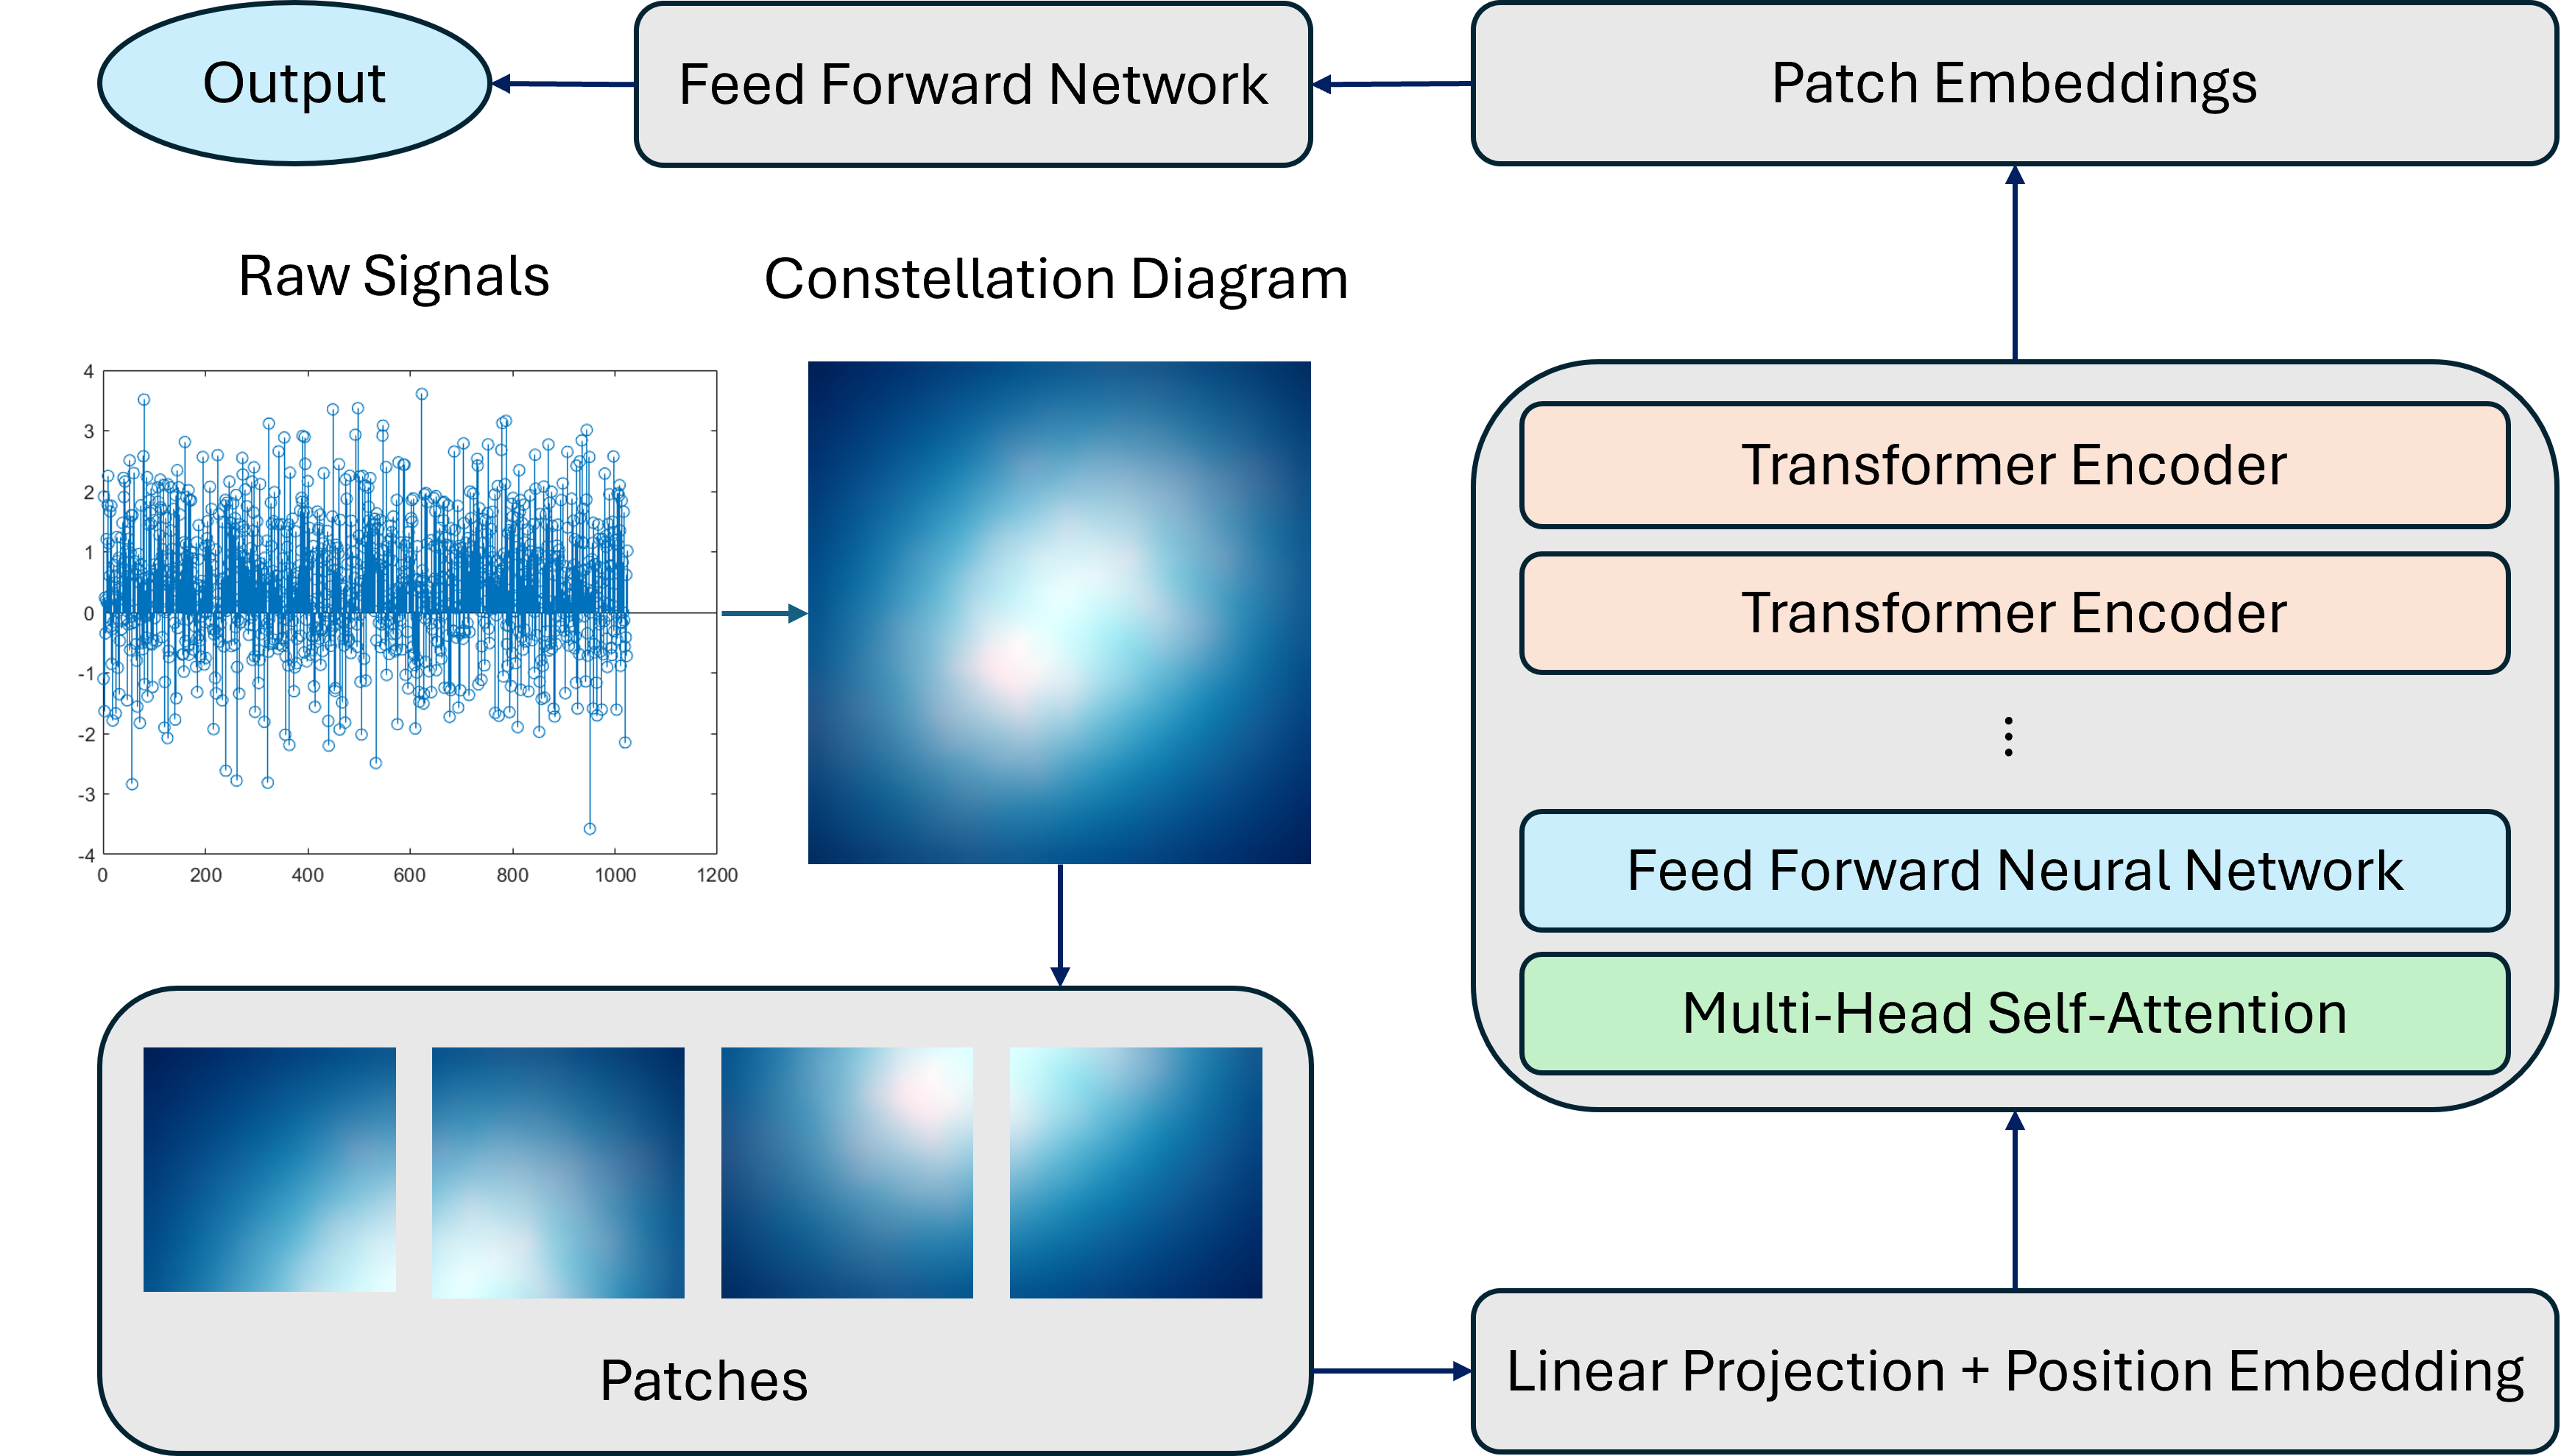
\includegraphics[width=\linewidth]{FIGURES/nmformer/nmformer.png}
    \caption{NMformer system sequential pipeline: starting with generating constellation diagrams from raw signals and culminating in modulation classification using a ViT architecture.}
    \label{fig:trans}
\end{figure} 

\subsubsection{Parameters Selection in Data Generation}

In all our experiments, we explore ten modulation formats. The samples are generated with dimensions of $32$ pixels for both height and width, equating to a sampling frequency of $200$ kHz. The constellation's scale for depiction is fixed at $2.5$. Furthermore, we incorporate reduced path delays of $0$, $0.0004$, and $0.0008$ seconds. The number of filter taps employed is $8$.

\subsubsection{Parameters Selection for Classifier}

For the NMformer, we adhere to most of the hyperparameters outlined in \cite{dosovitskiy2020image} for the network architecture. The input image size is configured to $224\times 224$, representing RGB images. Each input image is partitioned into $16$ equal square patches, which, in ViT, are regarded as tokens and processed by the transformer encoder. Each patch undergoes linear projection to the embedding dimension of $768$. The ViT model comprises $12$ transformer layers. The multi-head self-attention mechanism employs $12$ attention heads, facilitating simultaneous focus on different input segments. The dimensionality of the hidden layers within the feedforward networks in the transformer blocks is fixed at $3,072$.

The number of output classes is set to $10$ for the classification task, aligning with the ten modulation formats. We employ cross-entropy loss and an Adam optimizer with a learning rate $0.00005$. A consistent batch size of $128$ is utilized across all classifiers. The base classifier undergoes training for $50$ epochs, whereas the fine-tuned classifier is trained for $100$ epochs. We implement model saving based on the criterion of achieving the lowest validation loss or the highest validation accuracy, satisfying either condition.

\subsubsection{Base Classifier}

For the base classifier, we consider $11$ variations of SNRs ranging from $0$ dB to $10$ dB. Within each SNR, every training class comprises at least $1,000$ images and up to $1,100$ images. Hence, the total number of training samples amounts to $106,800$. We ensure that the validation set is generated with the same distribution as the training set, which contains samples from SNRs observed during training. Specifically, we generate samples with $4$ different SNRs for validation: $0$ dB, $4$ dB, and $8$ dB, with a total of $3,000$ samples.

During testing, we evaluate the classifier on two distinct datasets: one follows the in-sample distribution, where the data originates from the same SNRs seen during training, while the other is out-of-sample distribution data, comprising novel SNRs not encountered during training.

\subsubsection{Fine-tuned Classifier}

To refine the performance of the base classifier model for specific tasks with limited samples, we engage in fine-tuning the learned parameters. In this process, we freeze all layers of the NMformer except for the last linear layer. During fine-tuning, each SNR is associated with $100$ training samples for each class, contrasting with the base classifier, which has a minimum of $1,000$ samples per class. Post-fine-tuning, we evaluate the model's performance not only on novel classes but also on novel SNRs for both the base and fine-tuned classifiers. 

\subsection{Results and Discussion}

This section presents the test results derived from the base classifier trained over $100$ epochs. However, it is noteworthy that the model attains its optimal performance around the $40^{\mathrm{th}}$ epoch. Therefore, we save the model at this stage and evaluate its performance using the saved parameters. In our experiments, the out-of-distribution data typically presents a more challenging scenario for the classifier than the in-sample distribution. The outcomes are summarized in Table \ref{table:main}.

\begin{table}[htbp]
    \caption{Performance of the classifier on different settings.}
    \label{table:main}
    \centering
    \begin{tblr}{
      colspec={l l c c c c},
      hlines,
      vlines,
      cell{1}{1} = {c=2}{c},
      cell{1}{3} = {c=2}{c},
      cell{1}{5} = {c=2}{c},
      cell{2}{1} = {c=2}{c},
      cell{2}{3} = {c=2}{c},
      cell{2}{5} = {c=2}{c},
      cell{3}{1} = {c=2}{c},
      cell{3}{3} = {c=2}{c},
      cell{3}{5} = {c=2}{c},
      cell{5}{1} = {r=3}{c},
    }
    Model &               & Base           &             & Fine-tuned     &             \\
    Sample &             & 106{,}800      &             & 3{,}000        &             \\
    ~      &             & Accuracy (\%)  &             & Accuracy (\%) &             \\
    Distribution Type &  SNRs            & In          & Out            & In          & Out         \\
                     & 0 dB, 4 dB, 10 dB & 71.10       & -              & -           & -           \\
                     & 0.5, 1.5, 4.5 dB  & -           & 67.48          & 71.60       & 70.51       \\
                     & 5.5, 7.5, 9.5 dB  & -           & 72.12          & 75.77       & 71.87       \\
    \end{tblr}
    \end{table}


In the first test, we evaluated the performance of the base classifier using data from the same distribution. Specifically, the test classes included SNRs of $0$ dB, $4$ dB, and $10$ dB. The resulting test accuracy achieved in this scenario was \(71.10\%\).

Subsequently, we conducted tests on two out-of-distribution datasets. The first dataset comprises SNRs of $0.5$ dB, $1.5$ dB, and $4.5$ dB, where the lower SNRs pose greater challenges for classification. In this case, the obtained test accuracy is \(67.48\%\). Conversely, the second dataset contains SNRs of $5.5$ dB, $7.5$ dB, and $9.5$ dB, presenting less challenging classification tasks due to higher SNRs. Here, we achieved a test accuracy of \(72.12\%\).

The challenges posed by different SNR distributions are reflected in the accuracy results, where the less challenging distribution yields higher accuracy than the base classifier tested on all the in-distribution samples.

In the subsequent task, we fine-tune the base classifier using only a limited number of samples for specific SNRs. For the in-distribution SNRs of $0.5$ dB, $1.5$ dB, and $4.5$ dB, we achieve an accuracy of \(71.60\%\). Surprisingly, this surpasses the accuracy of the base classifier by \(0.50\%\), despite the samples having lower SNRs. This result demonstrates that our model can achieve higher accuracy when fine-tuned with a few yet challenging samples.

Conversely, when tested with higher SNR samples of $5.5$ dB, $7.5$ dB, and $9.5$ dB, the same fine-tuned classifier achieves an accuracy of \(71.87\%\). This accuracy is higher than that of the in-distribution samples, as higher SNR samples are less challenging to classify.

Furthermore, our test on the in-distribution samples of $5.5$ dB, $7.5$ dB, and $9.5$ dB yields the highest accuracy of all, \(75.77\%\). On the other hand, the out-of-distribution samples with SNRs of $0.5$ dB, $1.5$ dB, and $4.5$ dB achieve the lowest accuracy, which is \(70.51\%\). This lower accuracy is expected since the classifier is trained on fewer noisy samples, performing better on similar samples but experiencing a drop in accuracy for noisier ones. Nevertheless, this accuracy is \(3.03\%\) higher than that of our base classifier for the same distribution, demonstrating the superiority of our fine-tuned classifier.

We present the model convergence plots illustrating the smooth convergence of our fine-tuned model. These plots showcase the convergence behavior across different SNRs, specifically at $0.5$ dB, $1.5$ dB, and $4.5$ dB for the more challenging tasks and at $5.5$ dB, $7.5$ dB, and $9.5$ dB for the less challenging tasks.

Although the training and validation losses closely align in the first plot, they are noticeably higher compared to the latter plot. Consequently, the model achieves relatively lower accuracy at lower SNRs. However, across both plots, the model consistently converges towards the global minima as the training progresses.

\begin{figure}[htbp]
    \centering
    \begin{subfigure}[b]{0.48\textwidth}
        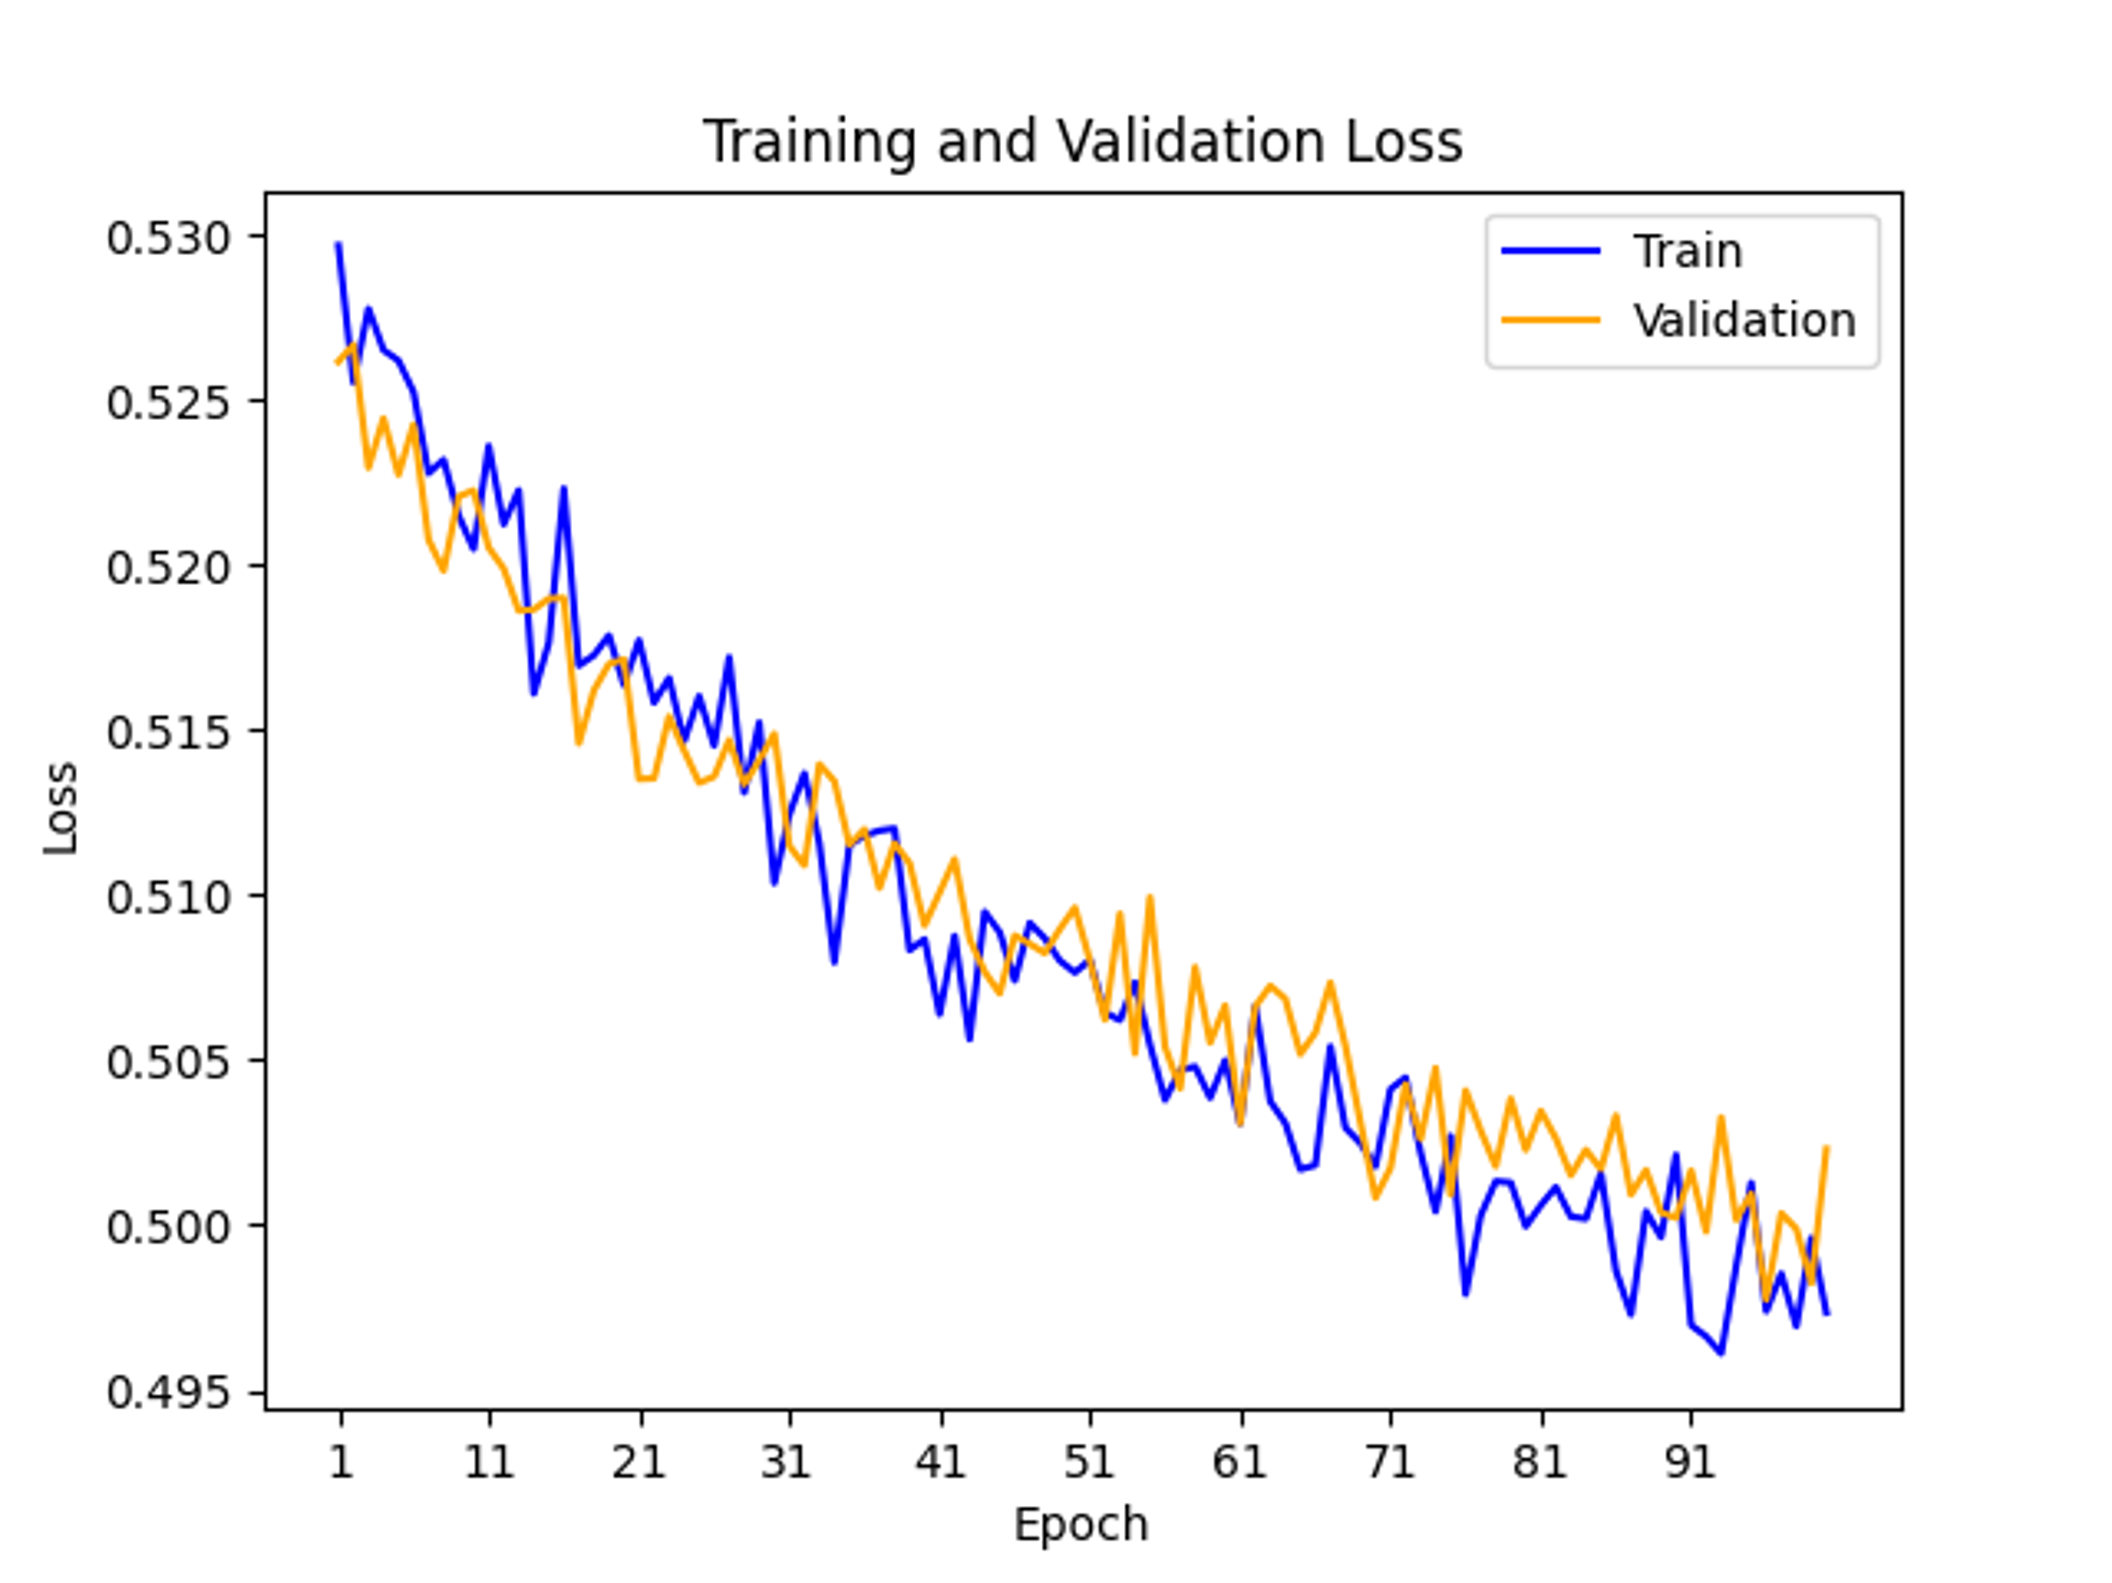
\includegraphics[width=\textwidth]{FIGURES/nmformer/loss_plot_l.png}
        \caption{Loss for 0.5 dB, 1.5 dB, and 4.5 dB SNRs.}
        \label{fig:sub1}
    \end{subfigure}
    \hspace{0.02\textwidth}
    \begin{subfigure}[b]{0.48\textwidth}
        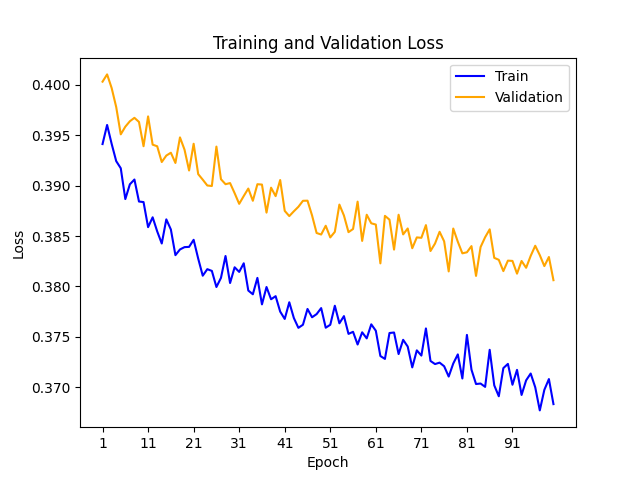
\includegraphics[width=\textwidth]{FIGURES/nmformer/loss_plot_h.png}
        \caption{Loss for 5.5 dB, 7.5 dB, and 9.5 dB SNRs.}
        \label{fig:sub2}
    \end{subfigure}
    \caption{Loss convergence plots across different SNR settings.}
    \label{fig:main}
\end{figure}

In Figure \ref{fig:conf}, we present the confusion matrices for our base classifier and two fine-tuned classifiers. Notably, all samples were misclassified for classes OOK and 16PAM in the base classifier. However, in Figure \ref{fig:conf}(b), corresponding to the fine-tuned classifier, we observe a notable increase in correctly classified samples for these classes. Subsequently, in Figure \ref{fig:conf}(c), there is a significant further increase in the number of correctly classified samples, indicating the clear superiority of our fine-tuned classifier.

To dive deeper into class performance analysis, we compute the classifier's precision, recall, and F1 score, as shown in Table \ref{table:pre}. The base classifier exhibits the lowest precision, recall, and F1 score among all classifiers. The precision, recall and F1 score values show improvement for both the fine-tuned classifiers. Notably, the fine-tuned classifier with a higher SNR achieves the highest F1 score, indicating superior performance across all evaluated metrics.

\begin{figure}[!htbp]
  \centering
  \begin{subfigure}[b]{0.55\textwidth}
    \centering
    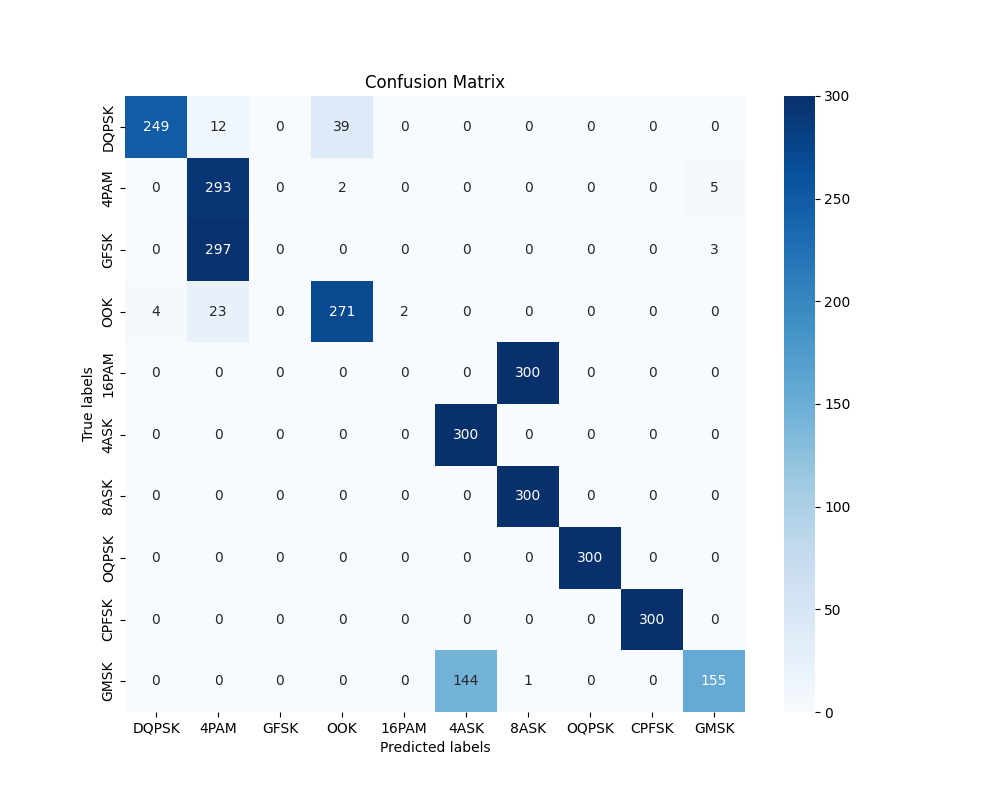
\includegraphics[width=0.7\textwidth]{FIGURES/nmformer/vit1_con.png}
    \caption{Base classifier.}
    \label{fig:subplot1}
  \end{subfigure}
  \begin{subfigure}[b]{0.55\textwidth}
    \centering
    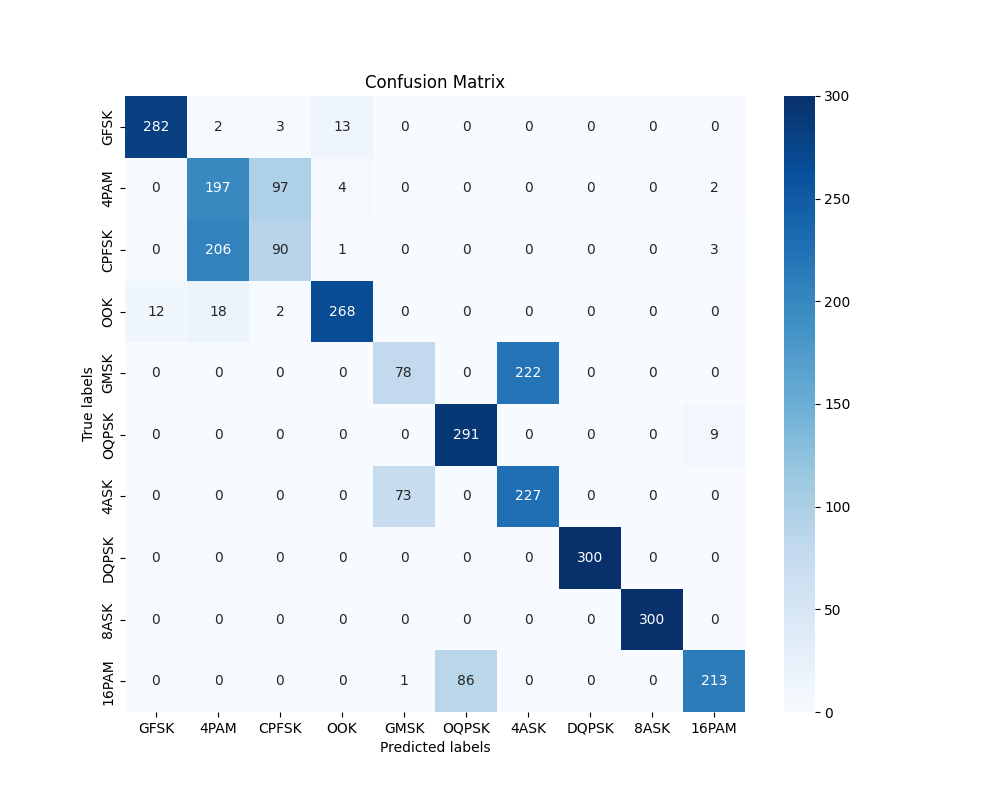
\includegraphics[width=0.7\textwidth]{FIGURES/nmformer/vit_f_p_con.png}
    \caption{Fine-tuned (0.5 dB, 1.5 dB, 4.5 dB).}
    \label{fig:subplot2}
  \end{subfigure}
  \begin{subfigure}[b]{0.55\textwidth}
    \centering
    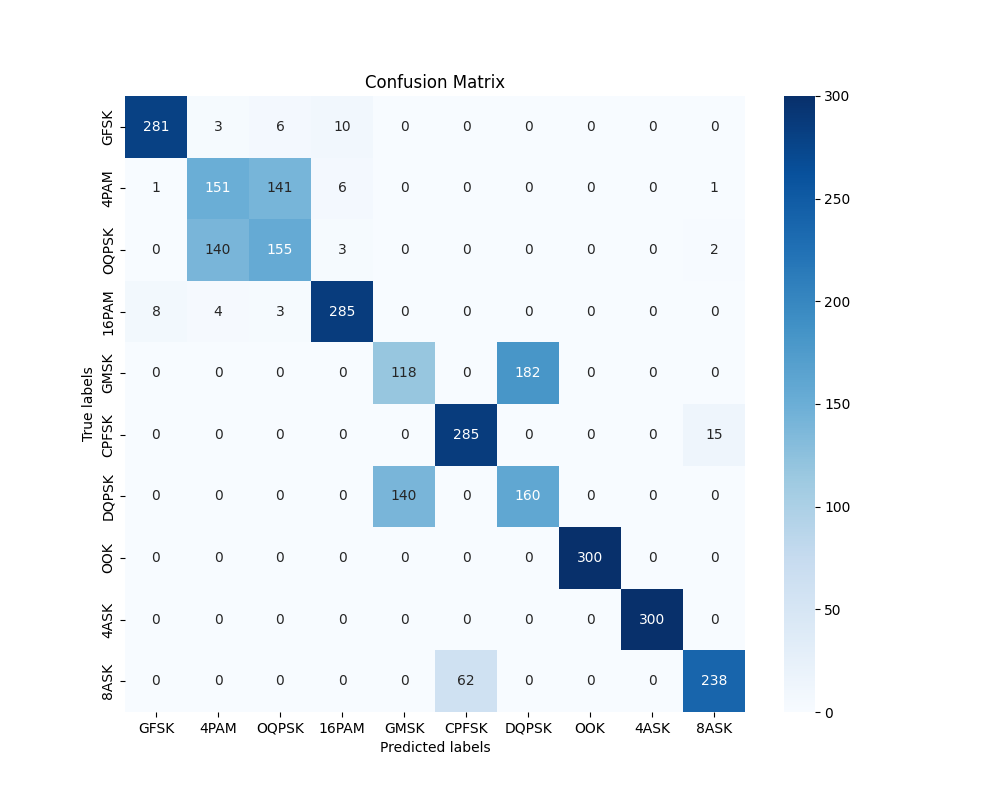
\includegraphics[width=0.7\textwidth]{FIGURES/nmformer/vit_f_p_h_con.png}
    \caption{Fine-tuned (5.5 dB, 7.5 dB and 9.5 dB).}
    \label{fig:subplot3}
  \end{subfigure}
  \caption{Confusion matrix for different classifiers.}
  \label{fig:conf}
\end{figure}

\begin{table}[htbp]
\caption{Analysis of classifier performance.}
\centering
\begin{tabular}{llll}
\hline
Classifier                             & Precision & Recall  & F1 Score \\
\hline
Base (0 dB – 10 dB)                    & 0.6170    & 0.6933 & 0.6291   \\
Fine-tuned (0.5 dB, 1.5 dB, 4.5 dB) & 0.7188    & 0.7163 & 0.7118   \\
Fine-tuned (5.5 dB, 7.5 dB, 9.5 dB) & 0.7598    & 0.7577 & 0.7572  \\
\hline
\end{tabular}
\label{table:pre}
\end{table}

\subsection{Conclusion}

In this study, we presented an effective model named NMformer for modulation classification in wireless communication systems leveraging a ViT model. Our proposed AMC method achieves remarkable accuracy across diverse SNRs by training on constellation diagrams of modulation signals. We demonstrate substantial improvement in classification performance by carefully fine-tuning the base classifier with limited samples tailored to specific SNRs. Our method surpasses the baseline classifier's accuracy and exhibits superior resilience to out-of-distribution data, particularly in challenging low SNR scenarios. The efficacy of our approach is further underscored by the precision, recall, and F1 score analyses, which consistently show significant improvements in classification metrics, particularly for classes traditionally prone to misclassification. Overall, our findings underscore the potentiality of NMformer for classifying noisy modulation signals.

\section{Task 2: DenoMAE: A Denoising Masked Autoencoder for Modulation Classification}

\subsection{Introduction}

Recent deep learning approaches have shifted toward addressing the high costs and scarcity of labeled data. Self-supervised learning has emerged as an efficient solution that leverages abundant raw data during pretraining, drastically reducing labeled data requirements while maintaining strong downstream performance \cite{balestriero2023cookbookselfsupervisedlearning}. These methods have shown remarkable success in natural language processing \cite{roberts2019exploring}, computer vision \cite{caron2021emerging} and other domains, opening new applications in fields with limited labeled data, including communications.

Wireless communication systems face critical challenges in maintaining reliable signal classification and interpretation, particularly in dynamic and noise-laden environments. Current approaches to modulation signal classification are predominantly supervised, requiring substantial amounts of labeled data across various Signal-to-Noise Ratios (SNRs) to achieve acceptable performance \cite{zheng2024deep}. These models often exhibit significant degradation when faced with previously unseen modulation types or noise conditions that deviate from their training distribution \cite{9965389}. This performance gap is striking in low SNR scenarios, where noise dominates the signal characteristics, leading to misclassifications and system failures \cite{perenda2021learning}. Despite advances in deep learning architectures for communications, the fundamental challenge remains: developing models that simultaneously maintain robustness to noise variation and generalize effectively with minimal labeled data requirements.

Existing solutions have explored several directions to address these challenges. Traditional denoising techniques treat noise as an unwanted component to be filtered out, often leading to information loss in the original signal \cite{shi2023gaf}. Single-modality masking approaches have shown promise in learning representations but fail to capture the complex interplay between signal characteristics and noise patterns. More recent multimodal learning approaches \cite{bachmann2022multimae, bachmann20244m} integrate data from multiple sources but typically treat noise as a distortion rather than an informative signal component. This fundamental limitation prevents these models from fully understanding the structural relationship between noise and signal modalities, restricting their ability to generalize across varying noise conditions. Additionally, most current methods require extensive labeled datasets across multiple SNR levels, making them impractical for rapidly evolving communication environments.

Our motivation stems from a key insight: noise in communication signals contains valuable structural information that enhances representation learning. By treating noise as an additional modality rather than a nuisance, we develop models that learn intrinsic relationships between clean signals and their noisy counterparts, enabling better generalization with less data. Building on this, we present DenoMAE, a multimodal autoencoder designed for communication systems that treats noise as an additional modality. This approach allows the model to generate all modalities from a single input, helping it comprehensively understand noise across modalities while enhancing denoising capabilities and learning robust signal representations. We employ random masking to challenge the model in reconstructing missing patches, reducing computational complexity while introducing beneficial uncertainty for effective learning.

\begin{figure}[htbp]
    \centering
    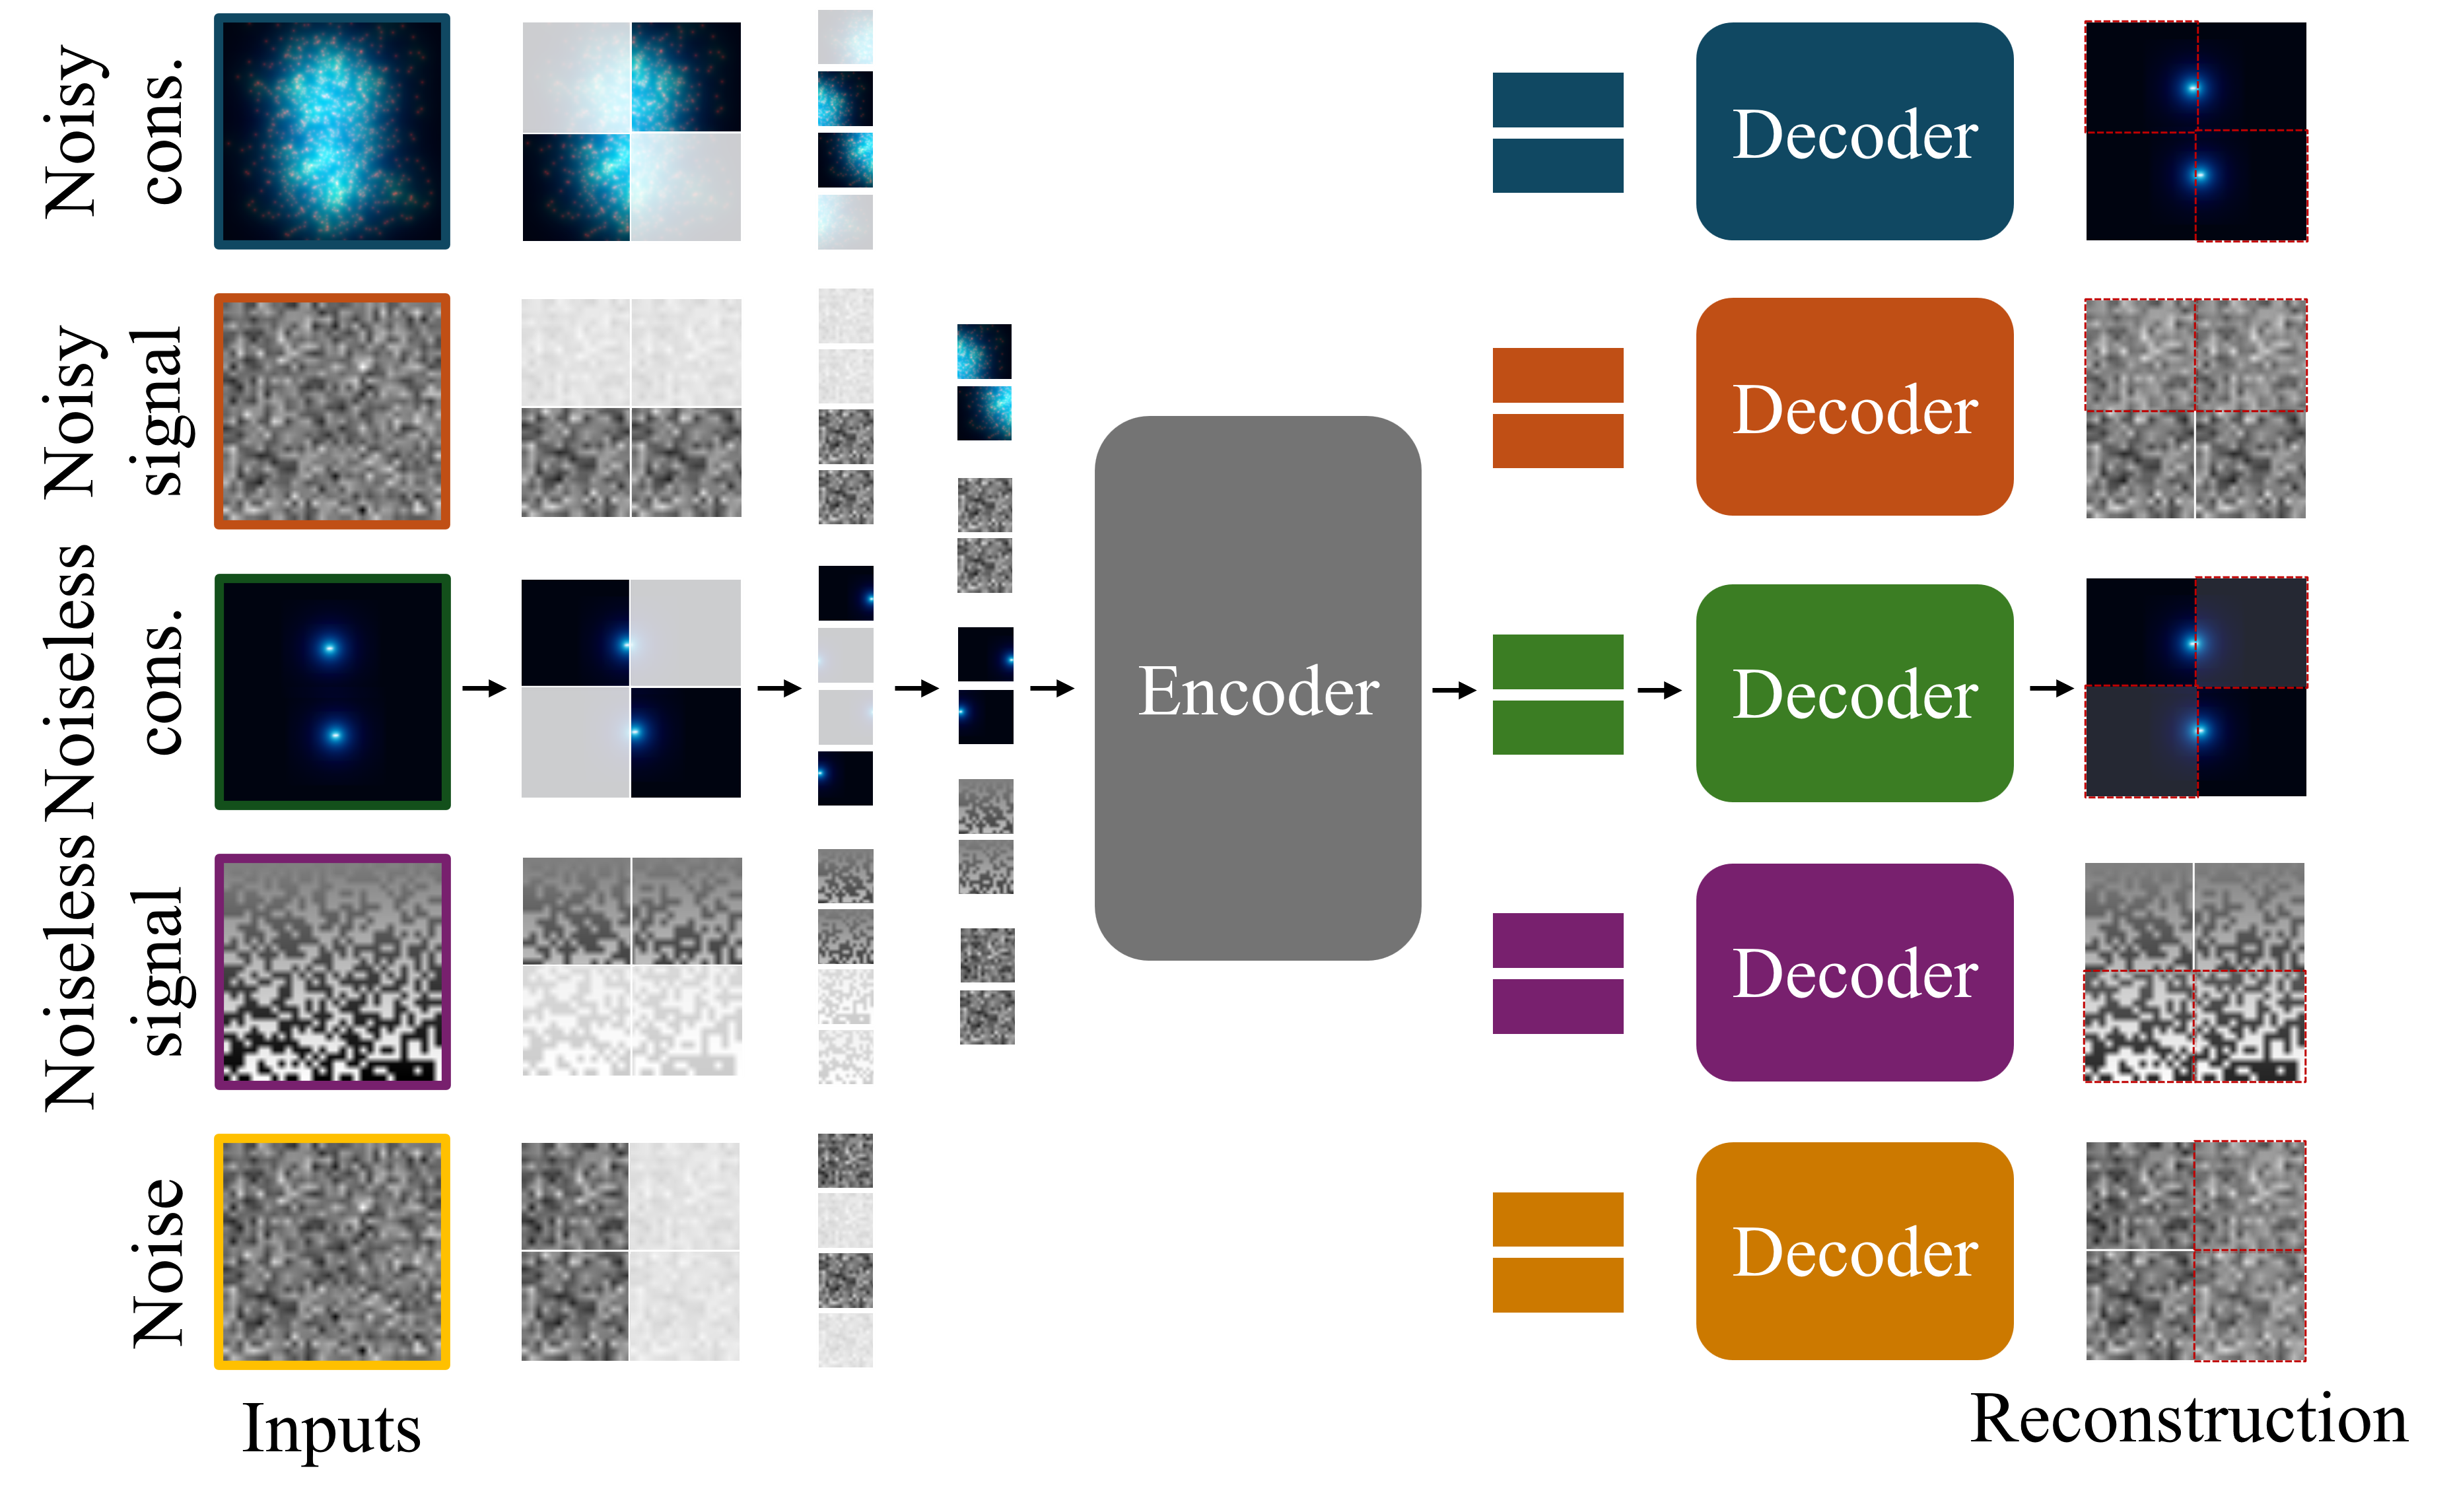
\includegraphics[width=\linewidth]{FIGURES/denomae/fig_new.png} % Adjust width as needed
    \caption{
    \textbf{DenoMAE Pretraining Strategy}: We apply a random 75\% masking \cite{he2022masked} (not to scale in the illustration) across all input modalities. The remaining 25\% of visible patches are processed by a shared encoder, while each modality utilizes a dedicated decoder to reconstruct its masked patches. Only the encoder is reused for fine-tuning the downstream tasks.
    }
    \label{fig:architecture} 
\end{figure}

\subsection{Contributtions}

Our contributions to DenoMAE are threefold:

\begin{itemize} 
\item We propose a novel multimodal paradigm that incorporates noise as an additional modality, enabling more effective pretraining on modulation signals and enhancing model resilience to noise. 
\item We demonstrate that our pre-trained model achieves significant improvements in classification accuracy under low SNR conditions, with accuracy gains of up to 22.1\% over non-pre-trained models. 
\item DenoMAE outperforms traditional methods, achieving superior results while requiring only one-tenth of the unlabeled data for pretraining and one-third of the labeled data for fine-tuning, underscoring its efficiency and scalability for real-world applications. 
\end{itemize}

\subsection{Related Work}

\textbf{Modulation Classification}: Recent advancements in deep learning have transformed AMC by enabling advanced analysis of constellation and other image diagrams. Much of the research emphasizes CNN-based architectures designed to classify modulation types while handling varying channel conditions \cite{huynh2020mcnet}. Innovative approaches include time-frequency adaptive decomposition with hybrid neural networks that reduce model parameters while maintaining accuracy and interpretability \cite{10945334}. Attention-based models like LSTMs and GRUs have evolved for processing modulation signals as time-series data \cite{8446021, liu2021automatic}, with transformer-based architectures gaining prominence for their ability to incorporate global sequence information \cite{kong2023transformer}. Transformer-deep recurrent hybrids have shown particular promises \cite{10668824}, while contrastive learning approaches have emerged to address generalization error and improve transferability under low SNR conditions \cite{10857965}. Recent semi-supervised frameworks combine transformers with contrastive learning to overcome labeled data limitations \cite{10093837}. Despite these advancements, many architectures still lack robustness across diverse noise scenarios, limiting their generalization beyond specific tasks.

\textbf{Multisensory Masked Modeling}: Masking large portions of the input and training the model to reconstruct or predict missing elements has become a popular self-supervised approach, especially within autoencoder-based methods. For example, BERT \cite{devlin2018bert} introduced masked language modeling by masking words in sentences and training the model to predict them, a concept adapted for vision with Masked Autoencoders (MAE) \cite{he2022masked}, where image patches are masked to encourage the model to learn robust visual representations. In multimodal contexts, masked modeling extends to tasks combining text, vision, and audio, promoting cross-modal understanding. For instance, Vision-Language Pretraining (VLP) models \cite{wang2022image} utilize masked language and vision modeling to jointly learn from masked image regions and text tokens. Additionally, image modality-centered models like MultiMAE \cite{bachmann2022multimae} and 4M \cite{mizrahi20244m} have demonstrated strong performance by pretraining on multiple image modalities and enhancing inference capabilities across diverse inputs. These multimodal masking methods have demonstrated significant gains in self-supervised learning, advancing model performance in tasks that benefit from multimodal reasoning.

\subsection{DenoMAE Architecture}

DenoMAE consists of four primary components: input embedding, encoder, shared latent space, and decoder. Figure \ref{fig:architecture} illustrates the overall architecture. Our codes are public at \url{https://github.com/atik666/denoMae/tree/master}.

\subsubsection{Input Embedding}

For each modality $m \in {1, ..., n}$, we represent the input as a $C$-channel image $X_m \in \mathbb{R}^{C \times H \times W}$. We divide each image into non-overlapping patches of size $p \times p$, resulting in $N = (H/p)^2$ patches per modality. Each patch is flattened and linearly projected to a $D$-dimensional embedding space:

\begin{equation}
E_m = [e^m_1, ..., e^m_N] + E_{pos}, \quad e^m_i \in \mathbb{R}^D
\end{equation}

where $E_{pos}$ represents learnable positional embeddings. Here, $e^m_i$ denotes the $i$-th patch embedding for modality $m$, and $N$ is the total number of patches per modality.

\subsubsection{Encoder}

The encoder $f_{\textrm{enc}}$ is a series of $L$ transformer blocks. We randomly mask a high proportion (e.g., 75\%) of the input patches for each modality. The encoder processes the visible patches:

\begin{equation}
H_m = f_{\textrm{enc}}([e^m_{i_1}, ..., e^m_{i_k}]), \quad i_j \in \text{visible patches}
\end{equation}

\subsubsection{Shared Latent Space}

To enable cross-modal learning, we project the encoded representations from all modalities into a shared latent space. We use a linear projection followed by layer normalization, $LN$:

\begin{equation}
Z_m = LN(W_m H_m + b_m)
\end{equation}

where $W_m$ is the projection matrix for modality $m$, $H_m$ is the encoded representation, and $b_m$ is the corresponding bias term.

The shared latent representation $Z_m$ is the concatenation of all modality-specific projections:
$Z_m = [Z_1; ...; Z_n]$.

\subsubsection{Decoder}

The decoder $f_{\textrm{dec}}$ reconstructs the masked patches for all modalities simultaneously. It takes the shared latent representation $Z_m$ as input and processes it through a series of transformer blocks. The output is then split into modality-specific representations and projected back to the original patch space:

\begin{equation}
\hat{X}_m = f_{\textrm{proj}_m}(f_{\textrm{dec}}(Z_m))
\end{equation}

where $f_{\textrm{proj}_m}$ is a modality-specific projection layer.

\subsubsection{Loss Function}

We employ a multi-modal reconstruction loss that combines individual losses for each modality:

\begin{equation}
\mathcal{L} = \sum_{m=1}^n w_m \mathcal{L}_m
\end{equation}

where $w_m$ is the weight for modality $m$, and $\mathcal{L}_m$ is the reconstruction loss for that modality. We use the Mean Squared Error (MSE) as the reconstruction loss.

\subsection{Fine-Tuning on Downstream Tasks}

After pretraining, we adapt the encoder for downstream tasks by removing the decoder and attaching a classification head. For modulation classification, we use a two-layer multi-layer perceptron network (MLP) with ReLU activation and dropout regularization. The process begins by embedding input patches and adding positional embeddings to form $x'$. The encoder processes these embeddings, and we apply global average pooling (GAP) to obtain representation $z$. This representation passes through the classifier to produce predictions $\hat{y}$:

\begin{equation}
\hat{y} = W_2(ReLU(W_1 \cdot GAP(f_{enc}(x')) + b_1)) + b_2
\end{equation}

During fine-tuning, we optimize the entire network using cross-entropy loss, with the pretrained encoder parameters updated at a reduced learning rate. 

\subsection{Experimental Setup}

To evaluate the effectiveness of DenoMAE in modulation classification tasks, we conducted a series of experiments under varying signal-to-noise ratio (SNR) conditions. Our experimental methodology encompasses data preparation, model architecture configuration, pretraining strategy, and fine-tuning protocols.

\subsubsection{Constellation Diagram Generation}

Constellation diagrams provide more informative visualization for modulation classification than raw signals \cite{doan2020learning}. The generation process involves mapping signals onto a complex plane across SNR ranges of $-10$ dB to $10$ dB. Our enhancement process involves two steps: creating a gray image that handles varying pixel densities, then developing enhanced grayscale images using an exponential decay model that accounts for sample positions and neighborhood influence. This model incorporates sample power, point-pixel distance, and decay rate parameters. For compatibility with DenoMAE's RGB input requirements, we generate three-channel images by creating distinct enhanced grayscale images from the same data samples, each with different exponential decay rates.

\subsubsection{Parameters in Sample Generation} 

The dataset comprises signals from ten modulation formats, each originally of length $L_0 = 1024$. To conform to the transformer's input dimensions, signals undergo a two-step preprocessing: (1) reshaping to $\mathbf{S}_1 \in \mathbb{R}^{32 \times 32}$, and (2) interpolation to $\mathbf{S}_2 \in \mathbb{R}^{224 \times 224}$. For formats with $L_0 > 1024$ (e.g., $L_\text{GMSK} = 8196$), signals are initially downsampled to $L_0$. To match the three-channel structure of constellation images $\mathbf{I} \in \mathbb{R}^{3 \times 224 \times 224}$, $\mathbf{S}_2$ is replicated across three channels, yielding $\mathbf{S}_3 \in \mathbb{R}^{3 \times 224 \times 224}$. All signals are sampled at $f_s = 200$ kHz, ensuring consistency across modulation formats.

\subsubsection{Parameters for DenoMAE}

The DenoMAE architecture processes $n=5$ modalities of input images $\mathbf{X} \in \mathbb{R}^{3 \times 224 \times 224}$, segmented into $16 \times 16$ patches. The model employs a transformer-based encoder-decoder structure with $d_\text{model} = 768$ embedding dimensions. The encoder consists of $L_e = 12$ layers, while the decoder uses $L_d = 4$ layers, both utilizing $h = 12$ attention heads. During training, a random masking strategy with $p_\text{mask} = 0.75$ is applied. The model is optimized using AdamW with learning rate $\eta = 10^{-4}$ over $100$ epochs, using batches of size $B = 64$. This flexible architecture allows for easy adaptation to various multi-modal denoising tasks.

\subsubsection{Finetuning Parameters}

The fine-tuning task adapts the pre-trained DenoMAE model for classification across $C = 10$ classes. The encoder $f_{\textrm{enc}}$ from DenoMAE, with a depth, $d_\text{model} = 768$, is used as a backbone, followed by a classifier head $H(\cdot)$ consisting of a two-layer MLP with hidden dimension 512 and dropout $p = 0.5$, for an input $X \in \mathbb{R}^{3 \times 224 \times 224}$. The model is trained for $N_{\textrm{epoch}} = 150$ epochs using Adam optimizer with learning rate $\eta = 10^{-4}$ and batch size $B = 32$. Training data undergoes normalization but no augmentation.

\subsection{Results and Discussion}

This section presents a comprehensive analysis of DenoMAE's performance across various signal-to-noise ratios and modulation schemes. We examine the model's reconstruction capabilities during pretraining, classification accuracy during fine-tuning, and comparative performance against baseline approaches. Our analysis particularly focuses on the performance improvements in low SNR environments, which represent the most challenging scenarios for modulation classification in real-world applications. Additionally, we investigate the data efficiency of our approach compared to traditional supervised methods.

\begin{figure}[htbp]
    \centering
    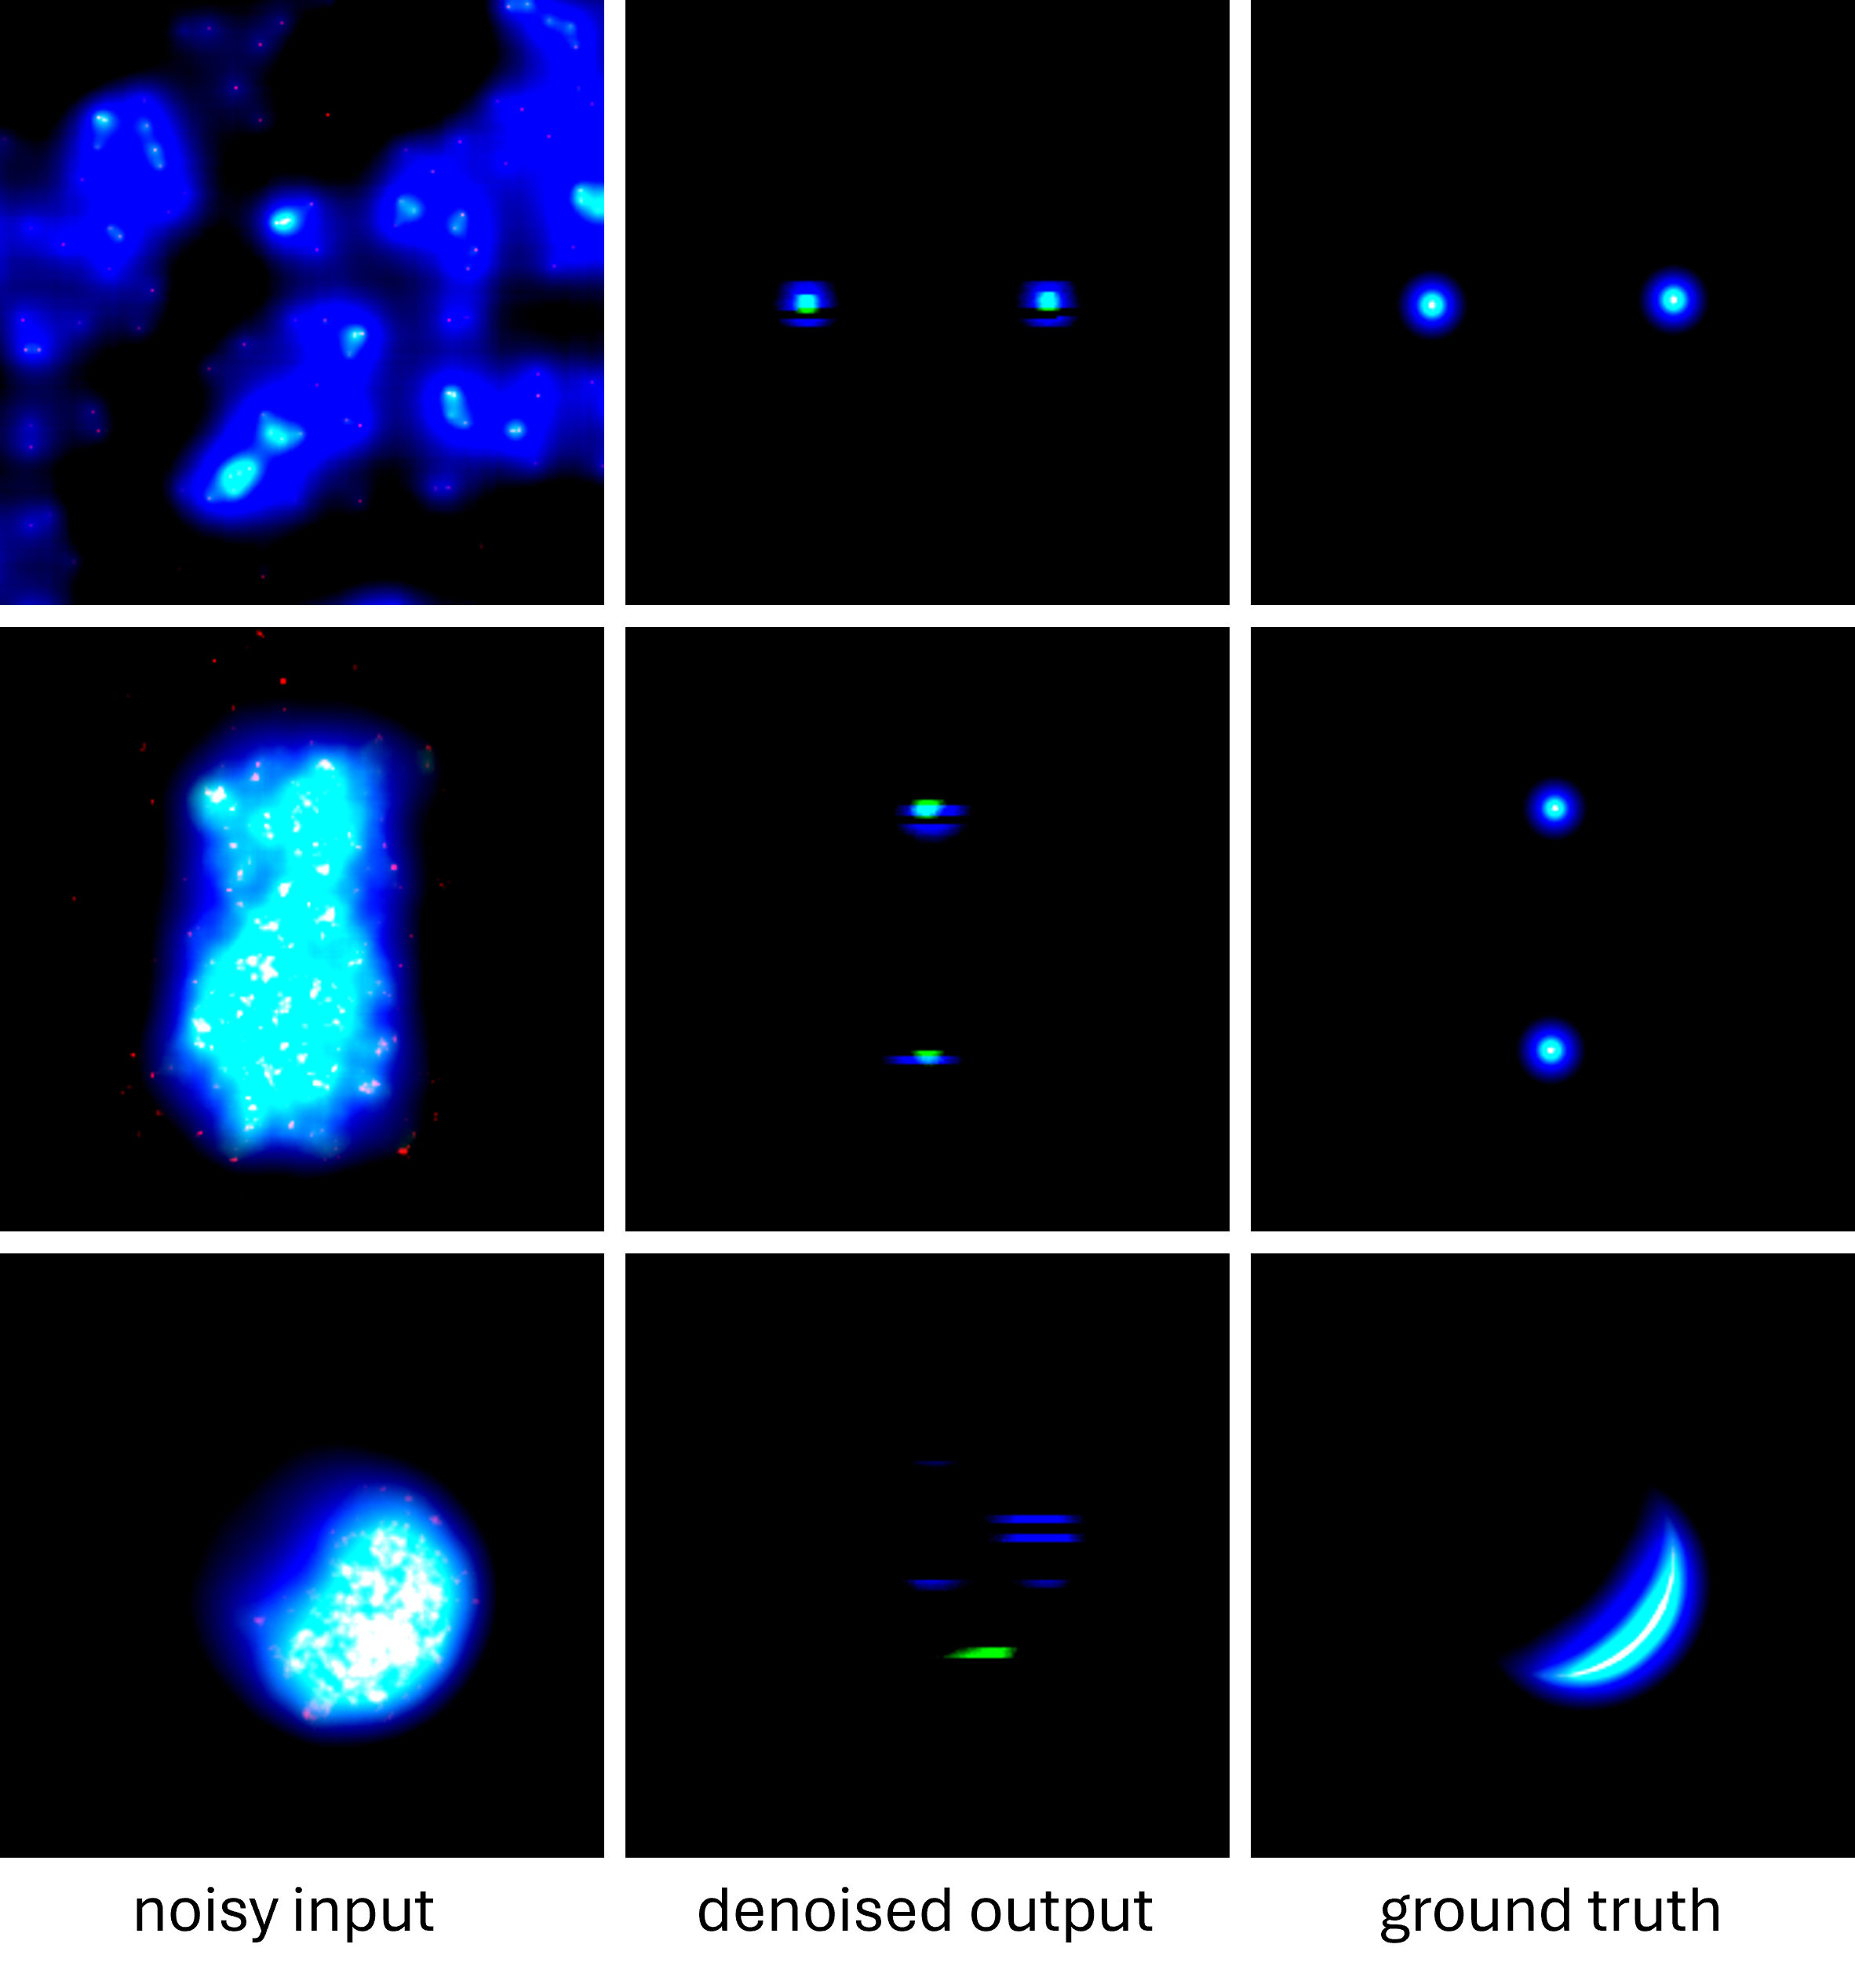
\includegraphics[width=0.75\linewidth]{FIGURES/denomae/outputs.png} 
    \caption{Denoised outputs on constellation diagrams at different SNRs.}
    \label{fig:outputs} % Label for referencing
\end{figure}

\subsubsection{Pretraining Performance}

The pretraining effectiveness of DenoMAE was evaluated using $10,000$ unlabeled signal samples across five modalities. We used 100 constellation samples equally distributed across classes as validation data during pretraining. Visual inspection of the denoised constellation diagram outputs (Figure \ref{fig:outputs}) demonstrates strong reconstruction capabilities, particularly for samples in the first two rows where the model successfully removes noise while preserving signal characteristics. While reconstruction quality slightly diminishes for samples in the last row, the overall shape and pattern retention remain sufficient for downstream tasks.

\subsubsection{Impact of SNRs}

In fine-tuning, we utilized a labeled dataset comprising of constellation images evenly distributed across classes. The dataset was partitioned into $1,000$ training images, $100$ validation images, and $100$ testing images, with 10 classes: 4ASK, 8ASK (Amplitude Shift Keying), 4PAM, 16PAM (Pulse Amplitude Modulation), CPFSK (Continuous Phase Frequency Shift Keying), DQPSK (Differential Quadrature Phase Shift Keying), GFSK (Gaussian Frequency Shift Keying), GMSK (Gaussian Minimum Shift Keying), OOK (On-Off Keying), OQPSK (Offset Quadrature Phase Shift Keying). The impact of SNR on classification performance reveals DenoMAE's robust noise resilience. As shown in Figure \ref{accuracy}, the pre-trained model achieves 77.50\% accuracy even at $-10$ dB SNR, with performance steadily improving to 84.30\% at $10$ dB. The pretraining advantage is most pronounced in challenging low-SNR conditions, demonstrating a 22.1\% improvement over the non-pre-trained baseline at $-10$ dB. This performance gap gradually narrows at higher SNRs, suggesting that pretraining is particularly valuable for learning noise-robust features.

\begin{figure}[htbp]
    \centering
    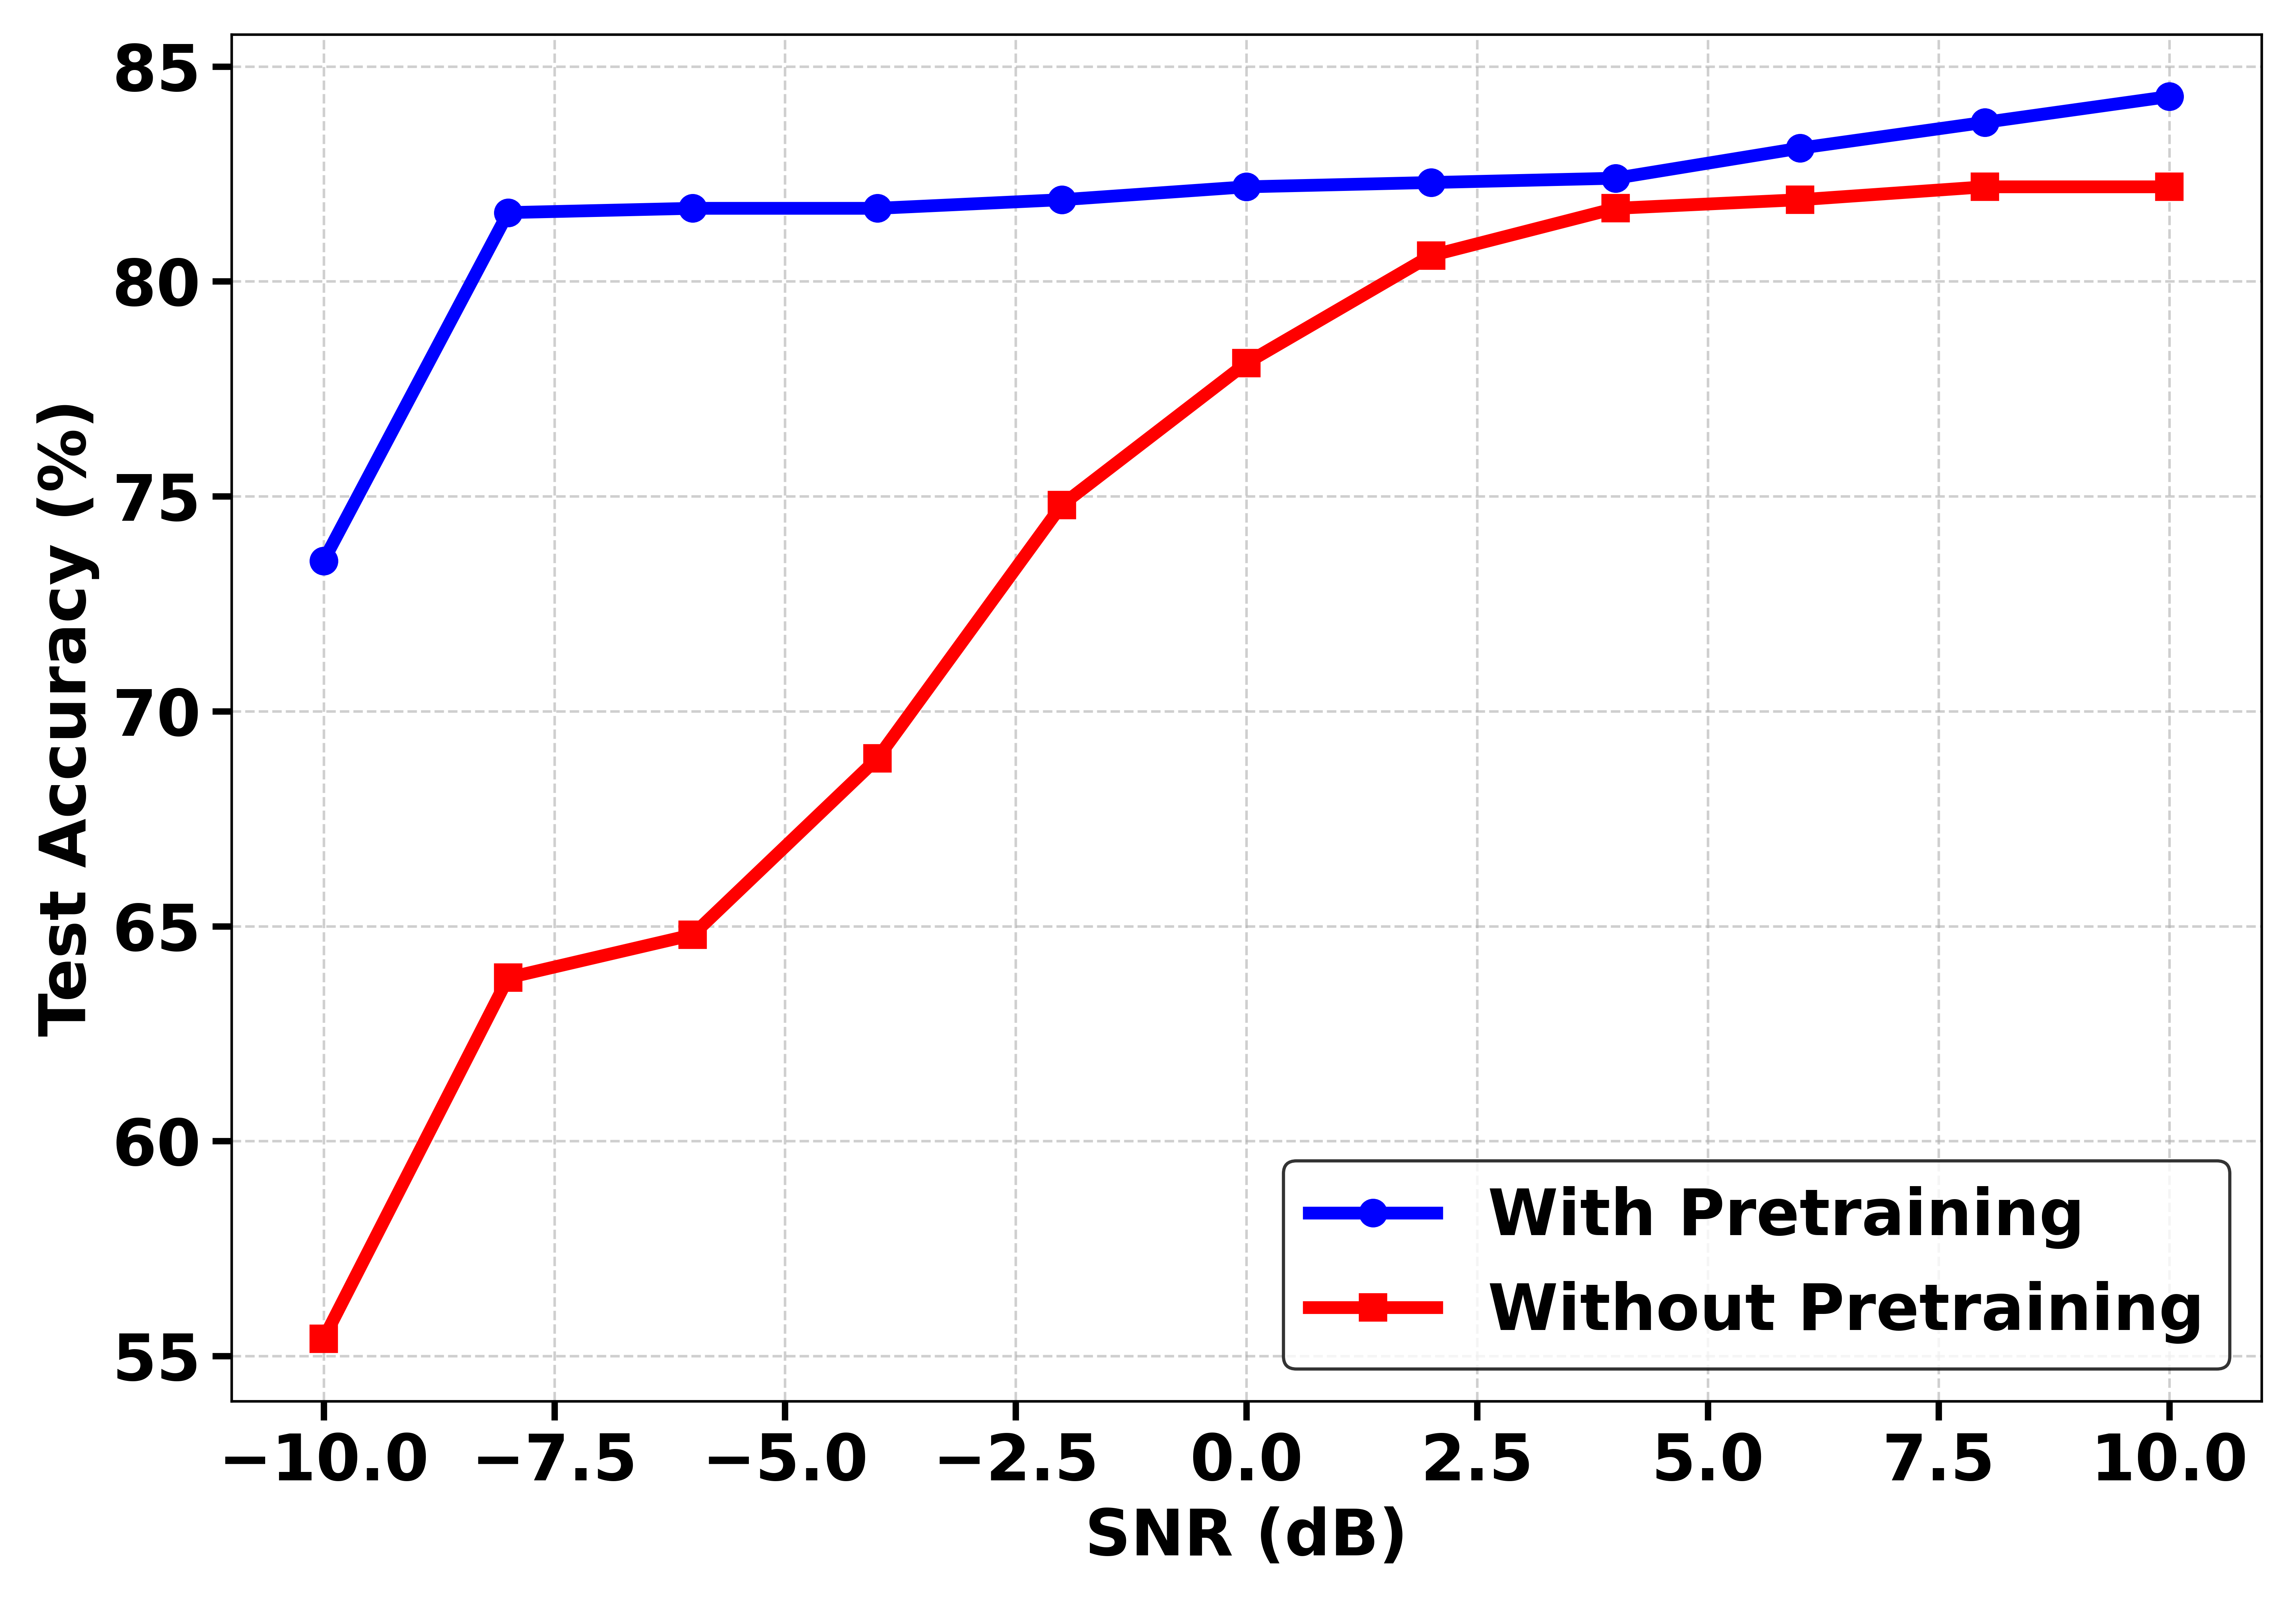
\includegraphics[width=0.85\linewidth]{FIGURES/denomae/plot.png} % Adjust width as needed
    \caption{Classification accuracy for constellation diagrams at different SNRs.}
    \label{accuracy} % Label for referencing
\end{figure}

\subsubsection{Effect of Masking Ratio}

We investigated the impact of masking ratio during pretraining on downstream classification. As shown in Figure \ref{masking}, masking ratio significantly influences performance, with accuracy rising from 79.6\% at 10\% masking to peak at 83.5\% with 75\% masking, before declining to 81.4\% at 80\% and 79.0\% at 90\% masking. This pattern indicates moderate to high masking ratios (60-75\%) compel the model to learn more robust features by reconstructing substantial missing information. Extremely high ratios (\textgreater{80\%}) provide insufficient context for effective reconstruction, while low ratios (\textless{40\%}) fail to sufficiently challenge the model. The optimal approach thus involves masking a significant but not overwhelming portion of input data.

\begin{figure}[htbp]
    \centering
    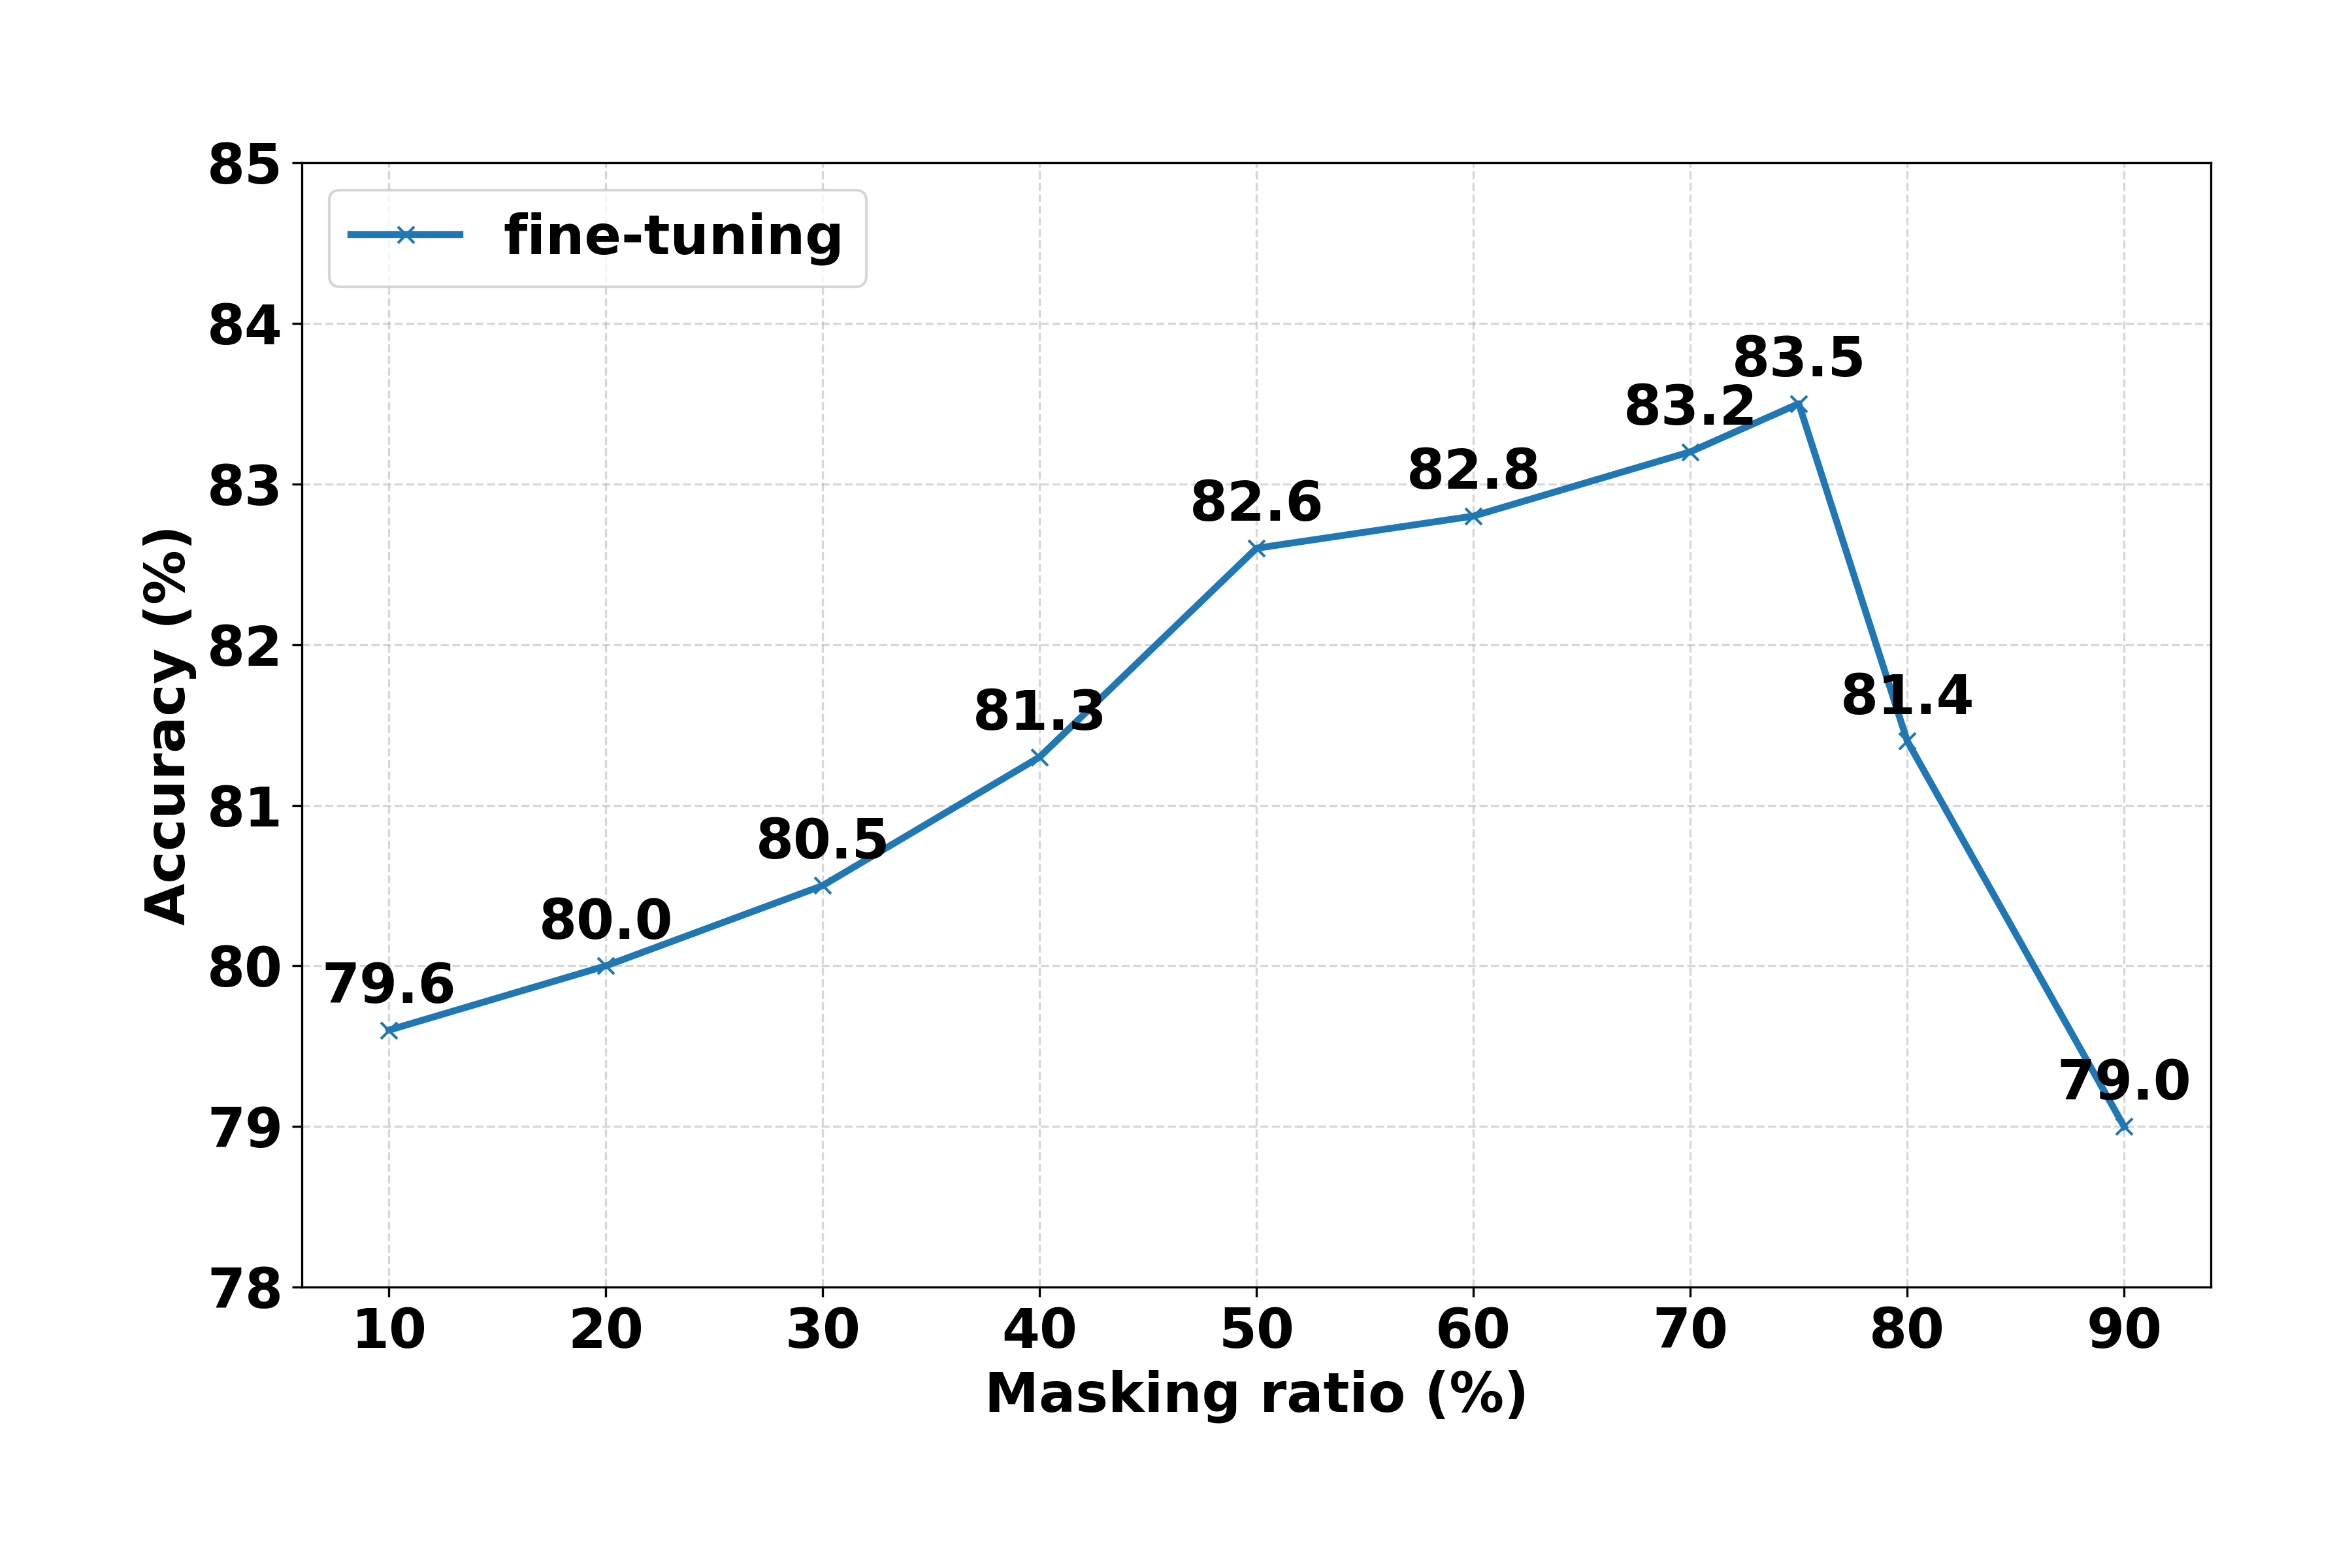
\includegraphics[width=0.9\linewidth]{FIGURES/denomae/mask.png} % Adjust width as needed
    \caption{Effect of masking ratio on fine-tuning accuracy.}
    \label{masking} % Label for referencing
\end{figure}

\subsubsection{Extrapolation on Out-of-bound SNRs}

DenoMAE demonstrates impressive extrapolation capabilities when evaluated on SNR conditions significantly outside its training range. Although trained only on SNR levels above $-10$ dB, the model continues to deliver meaningful reconstruction performance at challenging SNR levels between $-11$ dB and $-20$ dB. As shown in Figure \ref{fig:extrap}, DenoMAE effectively denoises highly noisy input constellation diagrams, making the first two samples visually recognizable. The final sample, while impacted by extreme noise, still approximates the outer shape of the ground truth.

\begin{figure}[htbp]
    \centering
    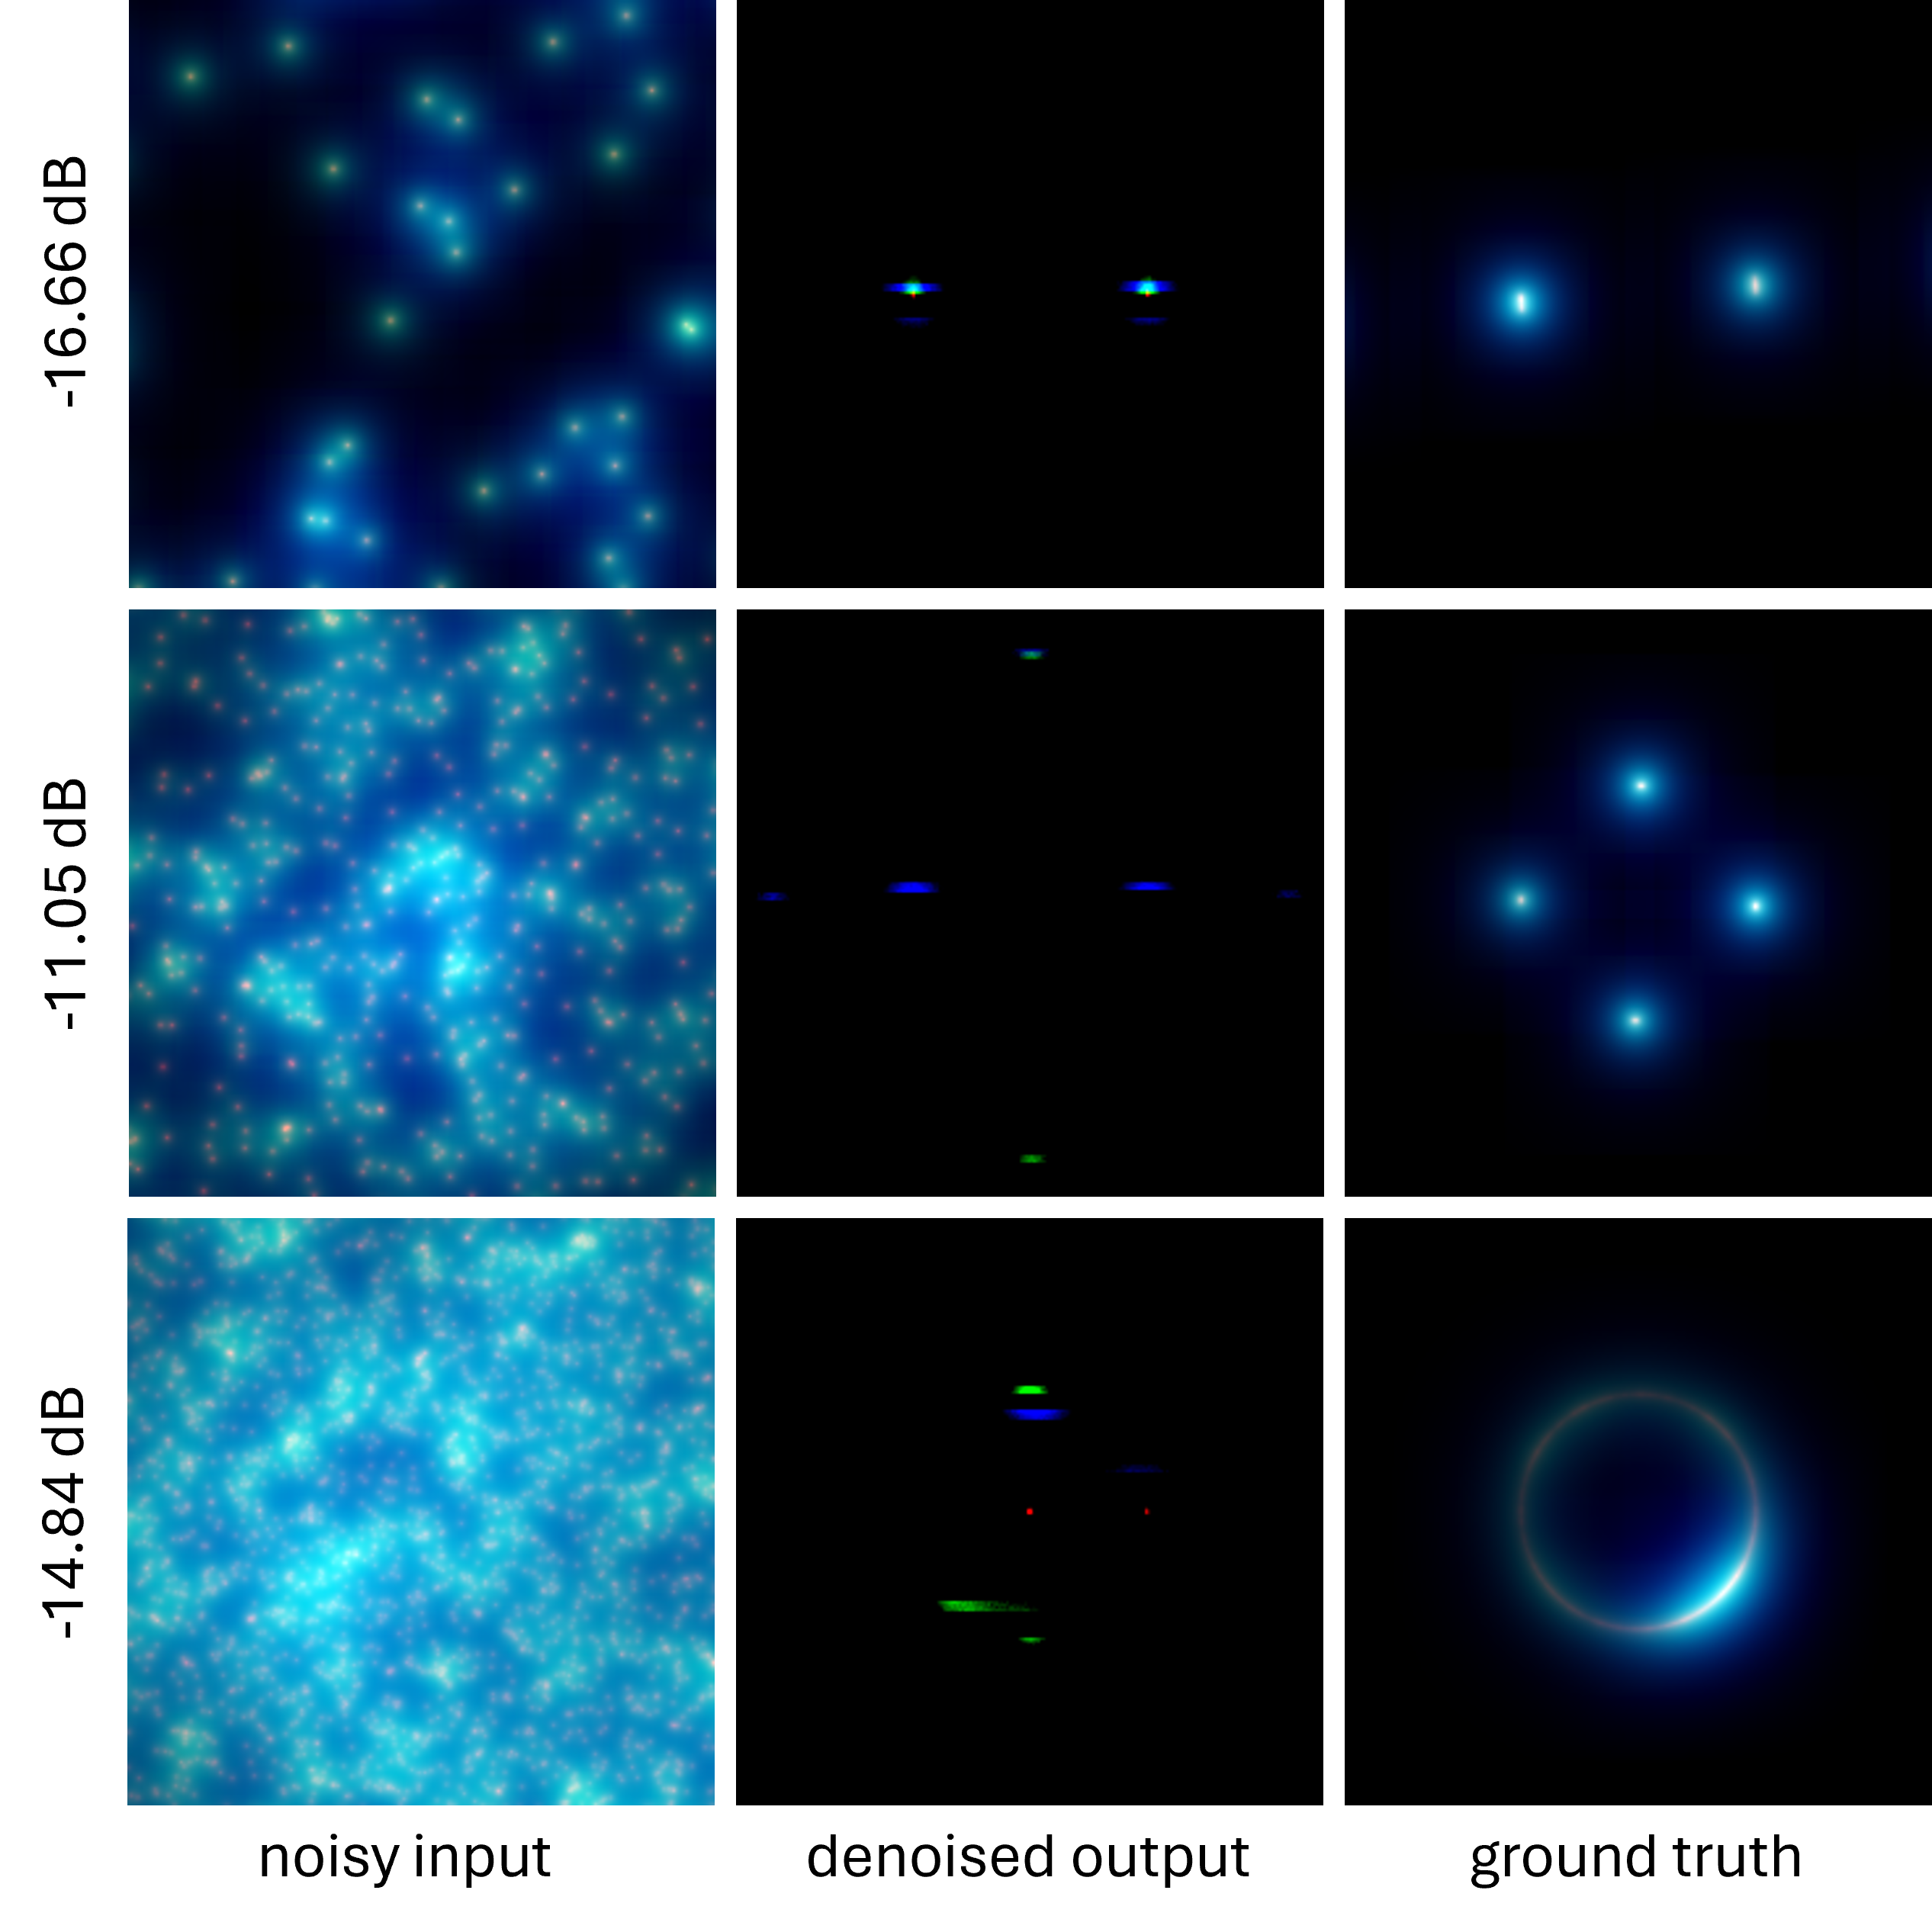
\includegraphics[width=0.8\linewidth]{FIGURES/denomae/extrapolate.png} % Adjust width as needed
    \caption{Extrapolation-ability of DenoMAE on out-of-bound lower SNRs.}
    \label{fig:extrap} % Label for referencing
\end{figure}

\subsubsection{Ablation Study on Modality Impact}

Our shared encoded space enables complementary information from different modalities to enhance each other through cross-modal knowledge transfer. When one modality (e.g., constellation diagrams) is severely corrupted by noise, the model can leverage information from the other modalities (e.g., signals) through this integrated representation. By aligning different views of the same signal in a common space, the model learns to distinguish between noise artifacts and true signal characteristics, significantly improving denoising performance.

Our ablation study on modality impact, detailed in Table \ref{modulations}, reveals the effectiveness of the multimodal approach. The full model with five modalities (noisy image, noisy signal, noiseless image, noiseless signal, and noise) achieves 83.50\% accuracy. Performance degrades gracefully as modalities are removed, with even the single-modality version maintaining 81.30\% accuracy. This suggests that while additional modalities contribute to performance gains, the model maintains robust performance even with reduced modality input, indicating efficient cross-modal learning capabilities.

\begin{table}
    \centering
    \caption{Performance Comparison Across Different Modalities}
    \label{modulations}
    \begin{tabular}{c|c|c|c|c|c}
    \hline
    \multicolumn{2}{c|}{Constellation} & \multicolumn{2}{c|}{Signal} & Noise & Test Accuracy (\%) \\
    \cline{1-4}
    Clean & Noisy & Clean & Noisy &  &  \\
    \hline
    \cline{1-4} 
    \checkmark &  &  &  &  & 81.30 \\
    \checkmark & \checkmark &  &  &  & 81.90 \\
    \checkmark & \checkmark & \checkmark &  &  & 83.20 \\
    \checkmark & \checkmark & \checkmark & \checkmark & & 83.30 \\
    \checkmark & \checkmark & \checkmark & \checkmark & \checkmark & 83.50 \\
    \hline
\end{tabular}
\end{table}
    
\subsubsection{Comparative Analysis}

Table \ref{compare} presents a comparison between DenoMAE and existing modulation classification approaches. Our model achieves 83.5\% accuracy at 0.5 dB SNR, outperforming AlexNet (82.8\% at 2 dB), NMformer (71.6\% at 0.5-4.5 dB), CNN-AMC (50.40\% at -6 dB), and DL-GRF (59\% at 0 dB). DenoMAE demonstrates remarkable data efficiency, requiring only 10,000 pretraining and 1,000 fine-tuning samples—an $80\times$ reduction compared to AlexNet's 800,000 samples and a $10.7\times$ reduction versus NMformer. Notably, DenoMAE maintains 77.50\% accuracy even at -10 dB SNR, highlighting its robust performance in challenging noise conditions.

From a computational perspective, DenoMAE has comparable model complexity to NMformer (both 85.8M parameters) with identical inference time (14.5 ms), yet delivers 11.9\% higher accuracy. While CNN-AMC offers faster inference (0.13 ms) with fewer parameters (1.6M), it achieves lower accuracy and classifies only 4 modulation types versus DenoMAE's 10 classes. Similarly, DL-GRF (23.5M parameters, 10 ms inference) handles only 4 classes. These results demonstrate DenoMAE's exceptional balance between performance, data efficiency, and complexity for real-world wireless communications.

\begin{table}[htbp]
    \centering
    \caption{Comparison of DenoMAE with other modulation classification methods}
    \label{compare}
    \resizebox{\textwidth}{!}{%
    \begin{tabular}{cccccccc}
    \toprule
    \multirow{2}{*}{\textbf{Methods}} &
    \multicolumn{2}{c}{\textbf{Number of samples}} &
    \multirow{2}{*}{\textbf{SNR dB}} &
    \multirow{2}{*}{\textbf{Number of classes}} &
    \multirow{2}{*}{\textbf{Finetuning parameters}} &
    \multirow{2}{*}{\textbf{Inference time (ms)}} &
    \multirow{2}{*}{\textbf{Test accuracy (\%)}} \\
    \cmidrule(lr){2-3}
    & \textbf{Pretraining} & \textbf{Fine-tuning} & & & & & \\ \midrule

    AlexNet\cite{peng2018modulation}  & 800,000 (train) & 8,000 (test)  & 2 & 8 & 22.5M & 2.0 & 82.8 \\
    NMformer \cite{faysal2024nmformer} & 106,800 & 3,000 & 0.5 - 4.5 & 10 & 85.8M & 14.5 & 71.6 \\
    CNN-AMC \cite{meng2018automatic} & 79,200 & 228,060 & -6 & 4 & 1.6M & 0.13 & 50.40 \\
    DL-GRF \cite{sun2022automatic} & 2,000 (train) & 200 (test) & 0 & 4 & 23.5M & 10 & 59 \\
    DenoMAE (\textbf{Ours}) & 10,000 & 1,000 & 0.5 & 10 & 85.8M & 14.5 & 83.5 \\
    DenoMAE (\textbf{Ours}) & 10,000 & 1,000 & -10 & 10 & 85.8M & 14.5 & 77.50 \\

    \bottomrule
    \end{tabular}%
    }
\end{table}

\subsection{Conclusion}

We presented DenoMAE, a multimodal autoencoder framework that achieves state-of-the-art performance in modulation signal denoising while requiring significantly less training data than existing approaches. Our experiments demonstrate that by incorporating multiple modalities and treating noise as an explicit modality, DenoMAE delivers superior classification accuracy and robust performance across varying SNR conditions, including extrapolation to out-of-bound low SNRs. Future work could explore its extension to diverse signal types and optimization for computational efficiency.

% TODO: Omitting DenoMAE2.0 for now.
% \section{Task 3: DenoMAE2.0: Improving Denoising Masked Autoencoders by Classifying Local Patches for Automatic Modulation Classification}

% \subsection{Introduction}

% Semi-supervised models have emerged as a transformative paradigm in machine learning, addressing the high costs associated with data labeling \cite{zhang2024maskmatch, pmlr-v182-poulain22a}. A prevalent approach in semi-supervised learning involves pretraining models on large amounts of unlabeled data, which are abundant and readily available \cite{chen2020bigselfsupervisedmodelsstrong, xu2022revisitingpretrainingsemisupervisedlearning}. These models leverage unlabeled data to capture underlying patterns and structures, enabling effective representation learning. Consequently, the pretrained models exhibit improved performance and faster adaptation during downstream tasks, making semi-supervised learning a cost-efficient and scalable solution for real-world applications \cite{cai2022semisupervisedvisiontransformersscale}.

% Recent advancements in self-supervised learning have achieved remarkable success through representation learning~\cite{grill2020bootstrap, chen2020exploring}, contrastive learning~\cite{chen2020simple, khosla2020supervised}, and masking strategies \cite{yin2024stablemask}. Among these, masking strategies leveraging Vision Transformer (ViT) \cite{dosovitskiy2020image} architectures have set new benchmarks in tasks such as classification , reconstruction, and image analysis. Masked Autoencoders (MAE) \cite{he2022masked}, in particular, have demonstrated significant potential by randomly masking portions of input data and training models to reconstruct the missing information. Despite their success, traditional MAE methods predominantly emphasize global reconstruction objectives, often neglecting fine-grained local patterns that are critical for enhancing representation learning \cite{yue2023understanding}.

% Masking strategies are particularly beneficial for pretraining in wireless communication for Autometic Modulation Classification (AMC), where acquiring labeled data is challenging due to privacy and copyright constraints \cite{zhao2024vit, zayat2023transformer}. Moreover, communication signals are often corrupted by environmental noise and channel losses, making robust representation learning essential. DenoMAE \cite{faysal2025denomae} addresses these challenges by integrating masking and denoising within a unified framework, leveraging masked modeling to enhance performance. While DenoMAE has demonstrated exceptional results in denoising and achieving strong classification accuracy, it inherits the fundamental principles of MAE, which focus primarily on global representation learning through masking. Consequently, the model remains unaware of the specific locations of the masked inputs, limiting its ability to fully exploit fine-grained local patterns and unlock the complete potential of representation learning.

% We present DenoMAE2.0, an enhanced framework that introduces a novel local patch classification objective alongside the traditional reconstruction task. Our approach differs from existing methods by treating visible patches as distinct classes based on their spatial positions, enabling the model to learn position-aware local features while maintaining global coherence. This dual-objective strategy encourages the model to capture both structural and semantic information, leading to more robust and informative representations.

% \subsection{Contributions}

% The key contributions of our work are threefold:

% \begin{itemize}
%     \item We propose a novel architecture that combines denoising reconstruction with local patch classification, enabling simultaneous learning of global and local features.
%     \item We introduce a position-based classification strategy that leverages spatial information to enhance representation learning without requiring additional labels.
%     \item Through extensive experiments, we demonstrate that DenoMAE2.0 achieves superior performance on various downstream and transfer learning tasks compared to traditional MAE and DenoMAE approaches, particularly in scenarios with limited labeled data.
% \end{itemize}

% Our results indicate that the integration of local patch classification significantly improves the quality of learned representations, leading to better denoising, generalization and faster convergence during fine-tuning. The proposed method not only advances the state-of-the-art in self-supervised learning but also provides insights into the importance of incorporating local structural information in representation learning frameworks.

% \subsection{Related Work}

% This section discusses recent advancements in modulation classification and self-supervised learning methods, with a focus on their applications in wireless communication systems. We examine how these approaches have evolved from traditional feature engineering to modern deep learning architectures, highlighting the growing importance of self-supervised techniques in addressing data scarcity challenges.

% \subsubsection{AMC in Wireless Communication}

% Early AMC methods primarily relied on expert-crafted features extracted from constellation diagrams and signal statistics, utilizing likelihood-based approaches and higher-order statistics to classify modulation schemes \cite{dobre2007survey}. Constellation diagrams, which visually represent symbol distributions in the complex plane, have been a fundamental tool for feature extraction in classical AMC. These diagrams illustrate the effects of noise, interference, and channel distortions, making them valuable for differentiating modulation schemes based on clustering patterns, symbol dispersion, and trajectory structures \cite{o2018over}. 

% The advent of deep learning revolutionized AMC by enabling models such as CNNs to operate directly on I/Q samples and constellation diagrams, bypassing the need for manual feature engineering \cite{zhang2021efficient}. Deep learning approaches leverage spatial patterns in constellation diagrams, learning robust representations that improve classification accuracy over conventional methods \cite{doan2020learning}. More recent advancements incorporate attention mechanisms and transformer architectures to capture long-range dependencies in signal patterns \cite{hamidi2021mcformer}. However, these deep learning-based AMC methods often require large labeled datasets and exhibit limited generalization across varying channel conditions, posing challenges for real-world deployment \cite{ya2022large}.

% \subsubsection{Self-Supervised Learning Approaches}

% The evolution of modern Self-Supervised Learning (SSL) strategies in deep learning and wireless communication has progressed through distinct phases, starting with contrastive learning, followed by representation learning, and more recently, the adoption of masking techniques.  Contrastive learning exemplified by SimCLR~\cite{chen2020simple} and MoCo \cite{he2020momentumcontrastunsupervisedvisual}, relied on distinguishing positive and negative sample pairs to learn robust feature representations, proving effective in image and signal processing tasks. This was followed by representation learning methods \cite{grill2020bootstrap, berthelot2019mixmatch}, which eliminated the need for negative samples by aligning representations of augmented views, enhancing efficiency and scalability. More recently, masking-based techniques \cite{devlin2019bert, he2022masked} have gained prominence by reconstructing masked portions of inputs, offering a powerful framework for learning from incomplete data \cite{faysal2025denomae}.

% In wireless communication, semi-supervised learning are particularly useful for modulation classification, where labeled data is often scarce due to the complexity of signal environments. Ma et al. \cite{ma2024refined} developed a semi-supervised framework leveraging pseudo-labeling, where a model trained on limited labeled modulation samples generates labels for unlabeled data, iteratively refining its performance across diverse modulation schemes. Another approach by Sifaou and Simeone \cite{sifaou2024semisupervisedlearningcrosspredictionpoweredinference} exploits Cross-Prediction-Powered Inference (CPPI) to enhance semi-supervised learning by mitigating the bias of synthetic labels. Their method refines ML-based predictions through tuned CPPI and meta-CPPI, achieving improved performance in tasks like beam alignment and indoor localization, particularly when labeled data is scarce. More related SSL methods in wireless communication includes convolution \cite{zhang2024sswsrnetsemisupervisedfewshotlearning, ermis2022cnn, pmlr-v77-longi17a} and transformer \cite{kong2023transformer, ren2022sigtefficientendtoendmimoofdm, kunde2023transformers} based SSLs.

% \subsection{Methodology: DenoMAE2.0}

% The overall framework of the proposed DenoMAE2.0 is illustrated in Figure \ref{fig:denomae2}. DenoMAE2.0 consists of three components: encoder, reconstruction denoising decoder, and local patch classification head. There are two complementary objectives: the denoising reconstruction objective and the local patch classification classification objective. Details are provided in Algorithm~\ref{lst:DenoMAE2.0} and introduced as follows.

% \begin{figure*}[ht]
%     \centering
%     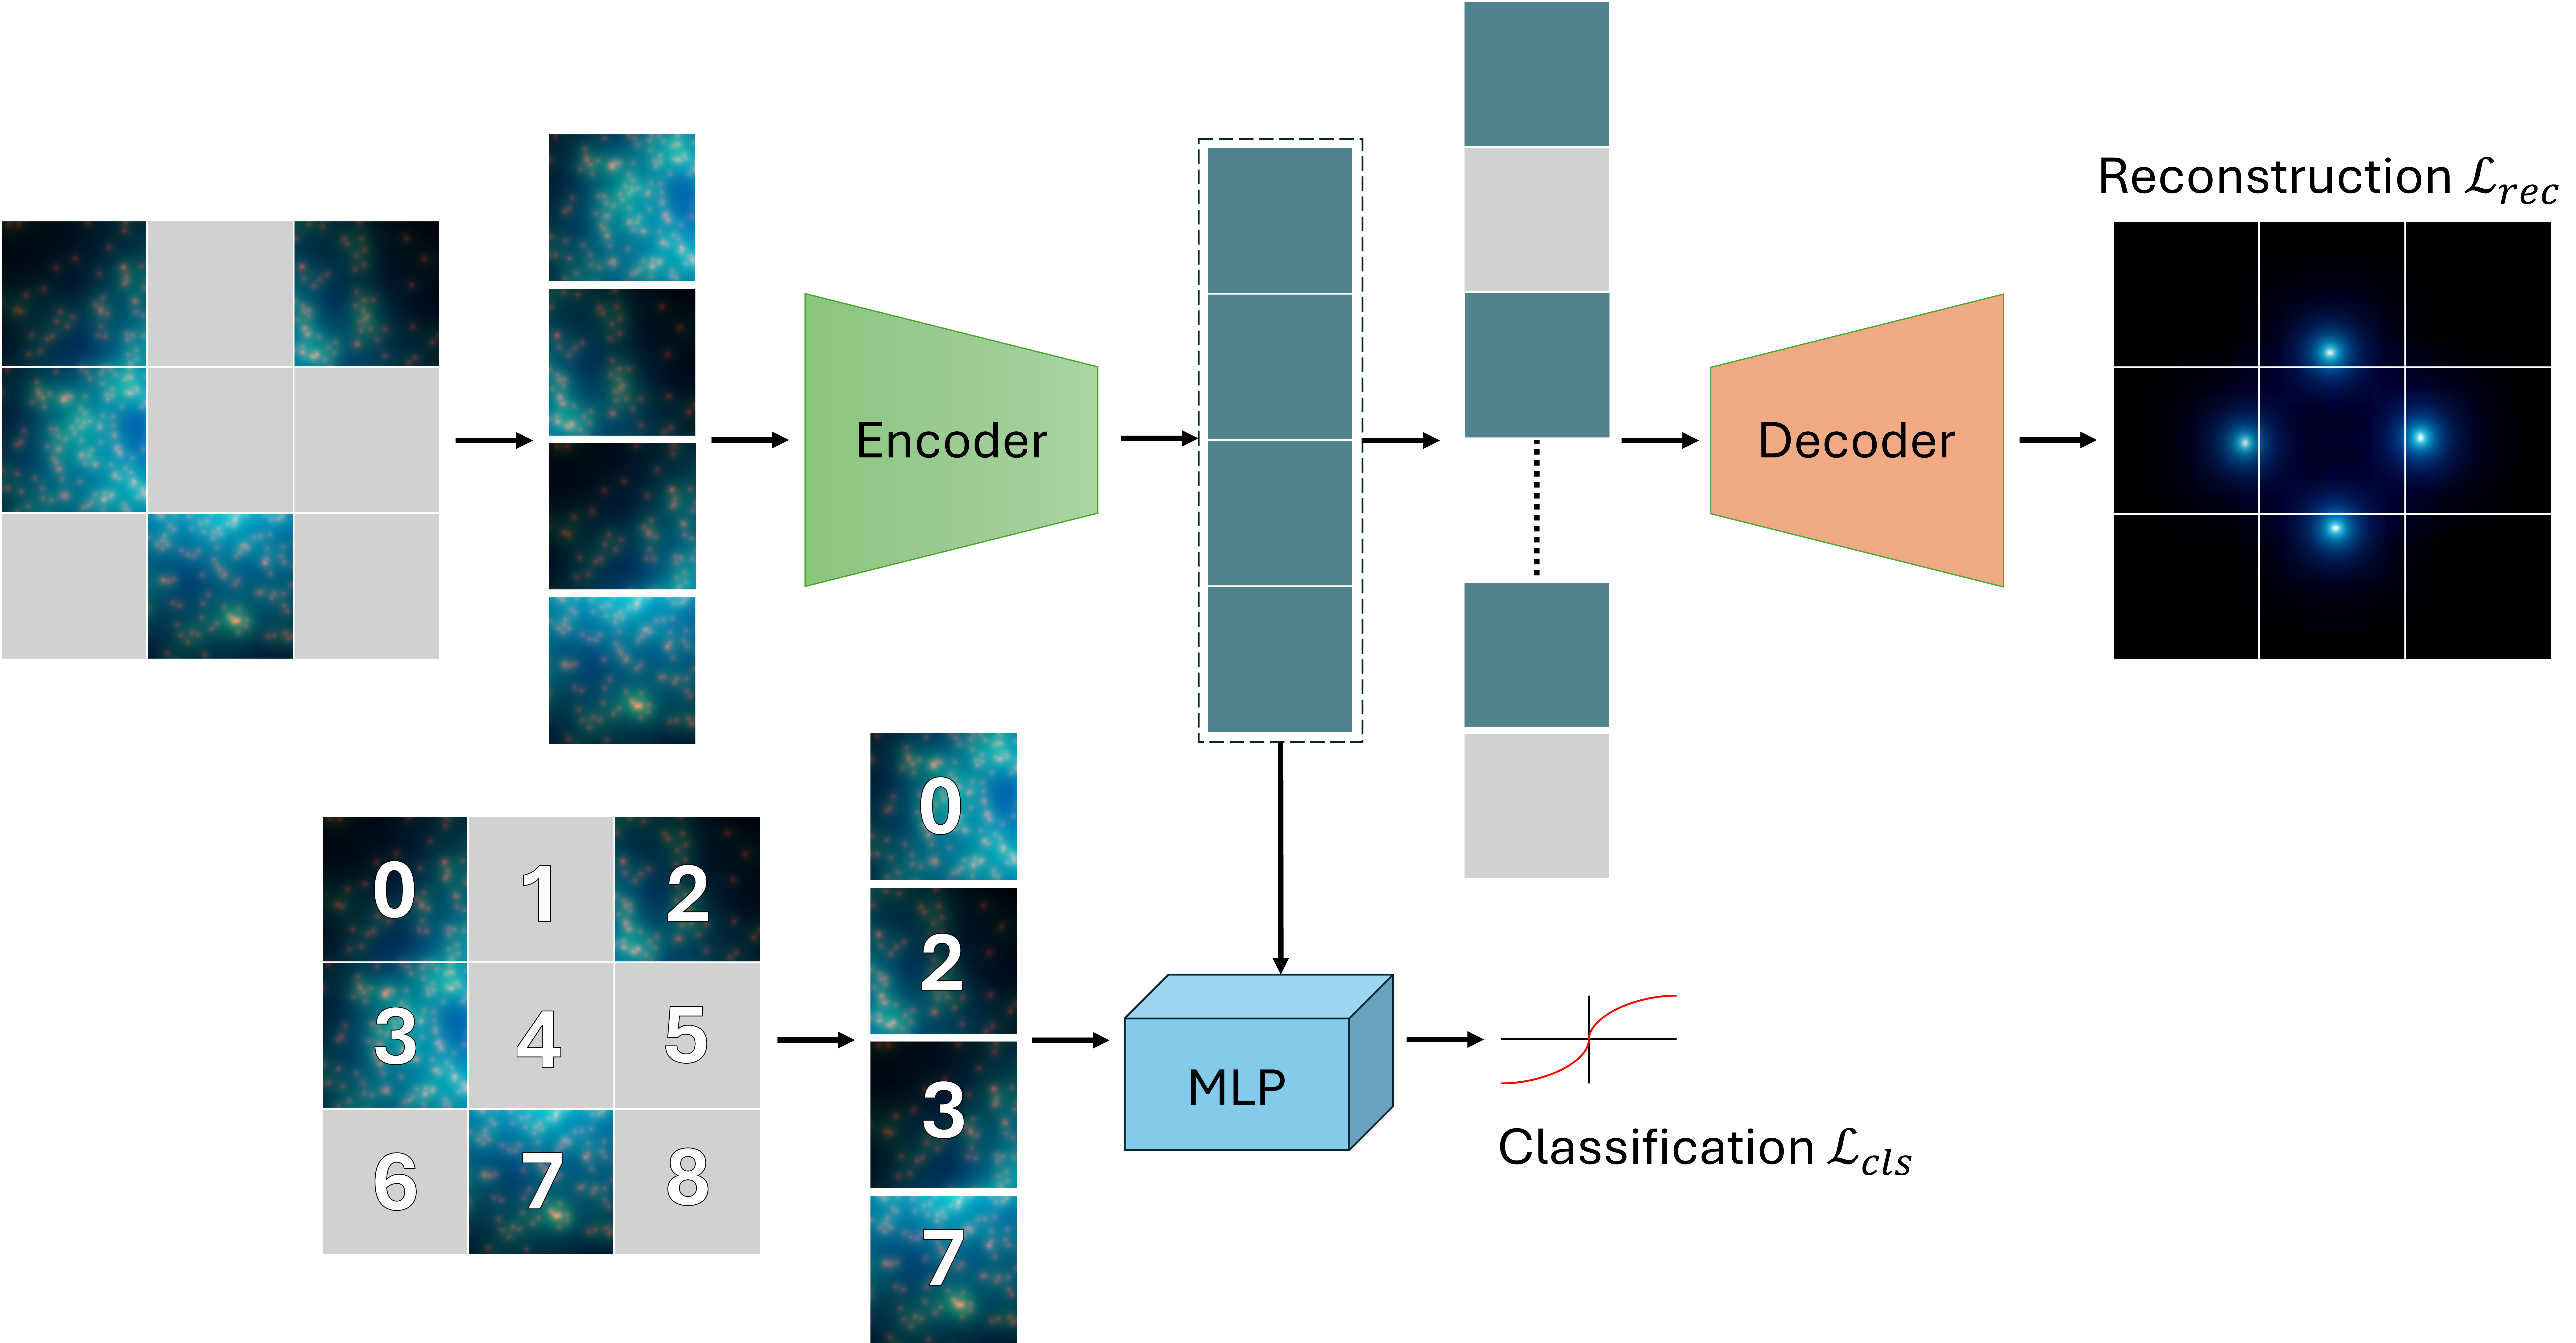
\includegraphics[width=0.9\textwidth]{FIGURES/denomae2/flow_con.png}
%     \caption{DenoMAE2.0 architecture overview: The model consists of an encoder-decoder architecture. The encoder processes visible patches and mask tokens, producing patch-level features for reconstruction and classification. The decoder generates reconstructed patches, while the classification head predicts patch position based on visible patch features.}
%     \label{fig:denomae2}
% \end{figure*}

% \subsubsection{Masking Strategy and Encoder Architecture}


% Consider an input image \(\mathbf{x} \in \mathbb{R}^{H \times W \times C}\). We first partition \(\mathbf{x}\) into 
% \begin{equation}
% N \;=\; \frac{H\,W}{P^2}
% \label{eq:num_patches}
% \end{equation}
% non-overlapping patches, each of size \(P \times P\). Let \(\mathbf{x}_p \in \mathbb{R}^{N \times (P^2\,C)}\) be the flattened patches. A linear projection \(E_{\mathrm{patch}}\) then maps these patches into a \(d\)-dimensional embedding space:
% \begin{equation}
% \mathbf{z}_p \;=\; E_{\mathrm{patch}}\bigl(\mathbf{x}_p\bigr) 
% \;\in\; 
% \mathbb{R}^{N \times d}.
% \label{eq:patch_embed}
% \end{equation}
% To preserve spatial order, we add learnable positional embeddings \(\mathbf{p} \in \mathbb{R}^{N \times d}\), forming the initial token sequence
% \begin{equation}
% \mathbf{Z}^{(0)} 
% \;=\; 
% \mathbf{z}_p 
% \;+\; 
% \mathbf{p}.
% \label{eq:pos_embed}
% \end{equation}

% A random masking operator \(\mathcal{M}_{r}\) discards a fraction \(r\) of these tokens to yield the visible tokens \(\mathbf{Z}_{v}\). The masked tokens \(\mathbf{Z}_{m}\) are replaced by mask tokens in the decoder but are omitted here in the encoder. Let \(\mathcal{E}\) denote the ViT-based encoder with \(L\) Transformer layers. Each layer \(\ell\) applies multi-head self-attention (MSA) and a feed-forward network (FFN) to the visible tokens:
% \begin{align}
% \mathbf{Z}_{v}^{(\ell)} 
% &=\; 
% \mathbf{Z}_{v}^{(\ell-1)} 
% \;+\;
% \mathrm{MSA}
% \!\Bigl(\mathrm{LN}\bigl(\mathbf{Z}_{v}^{(\ell-1)}\bigr)\Bigr),
% \label{eq:msa}
% \\[6pt]
% \mathbf{Z}_{v}^{(\ell)} 
% &=\; 
% \mathbf{Z}_{v}^{(\ell)} 
% \;+\;
% \mathrm{FFN}
% \!\Bigl(\mathrm{LN}\bigl(\mathbf{Z}_{v}^{(\ell)}\bigr)\Bigr).
% \label{eq:ffn}
% \end{align}
% After \(L\) layers, the encoder produces latent representations
% \begin{equation}
% \mathbf{q}_{v} 
% \;=\; 
% \mathcal{E}\bigl(\mathbf{Z}_{v}\bigr),
% \label{eq:encoder_output}
% \end{equation}
% which are subsequently used for both reconstruction in the decoder and the auxiliary classification of unmasked patches.


% \subsubsection{Decoder Architecture and Reconstruction}

% To reconcile the difference between the visible token set 
% \(\mathbf{Z}_{v}\) (equation \eqref{eq:encoder_output}) and the full 
% patch set of size \(N\) (equation \eqref{eq:num_patches}), we introduce 
% learnable \emph{mask tokens} at the masked positions. These tokens, 
% which share a single learned embedding, act as placeholders for the 
% missing patches. Formally, let 
% \(\mathbf{M} \in \mathbb{R}^{|\mathcal{I}_m| \times d}\) be the mask token 
% embeddings corresponding to the set of masked indices \(\mathcal{I}_m\), 
% where \(\mathcal{I}_v \cup \mathcal{I}_m = \{1,2,\dots,N\}\) and 
% \(\mathcal{I}_v \cap \mathcal{I}_m = \varnothing\). We concatenate the 
% visible patch embeddings \(\mathbf{q}_{v}\) and \(\mathbf{M}\), then add 
% positional embeddings to form the decoder input:
% \begin{equation}
%     \mathbf{Z}_{d}^{(0)}
%     \;=\;
%     \mathrm{Shuffle}\!\Bigl(\bigl[\mathbf{q}_{v} \;\Vert\; \mathbf{M}\bigr]\Bigr)
%     \;+\; 
%     \mathbf{p}_{d},
% \label{eq:decoder_input}
% \end{equation}
% where \(\mathbf{p}_{d} \in \mathbb{R}^{N \times d}\) denotes the positional 
% embeddings for the decoder, and \(\mathrm{Shuffle}(\cdot)\) reorders the tokens 
% to match their original patch indices.

% The decoder consists of a Transformer stack with fewer layers and heads 
% than the encoder for computational efficiency. Denote the decoder by 
% \(\mathcal{D}\). Each layer follows the same multi-head self-attention and 
% feed-forward structure described in \eqref{eq:msa}--\eqref{eq:ffn}, yielding 
% a final decoder output \(\mathbf{Z}_{d}^{(L')}\). A linear projection 
% \(\mathbf{W}_{\mathrm{out}} \in \mathbb{R}^{d \times (P^2\,C)}\) maps each token 
% to the original patch dimension, thereby producing reconstructed patches:
% \begin{equation}
%     \widehat{\mathbf{x}}
%     \;=\;
%     \bigl[\mathbf{Z}_{d}^{(L')} \mathbf{W}_{\mathrm{out}}\bigr]
%     \;\in\;
%     \mathbb{R}^{N \times (P^2\,C)}.
% \label{eq:decoder_out}
% \end{equation}

% We adopt a \emph{masked} mean squared error (MSE) loss to focus the 
% reconstruction objective solely on the masked patches. Let 
% \(\widehat{\mathbf{x}}_{m}\) and \(\mathbf{x}_{m}\) respectively denote the 
% reconstructed and ground-truth patches for the set of masked indices 
% \(\mathcal{I}_m\). The reconstruction loss is
% \begin{equation}
%     \mathcal{L}_{\mathrm{rec}}
%     \;=\;
%     \frac{1}{|\mathcal{I}_m|}
%     \sum_{i \in \mathcal{I}_m}
%     \bigl\|\widehat{\mathbf{x}}_{m}^{(i)} - \mathbf{x}_{m}^{(i)}\bigr\|^{2},
% \label{eq:rec_loss}
% \end{equation}
% where \(\|\cdot\|\) denotes the Euclidean norm. By confining 
% \(\mathcal{L}_{\mathrm{rec}}\) to the masked regions, the decoder is compelled 
% to infer the missing patches from context, thus enhancing its denoising 
% capabilities.


% \subsubsection{Patch Classification Head}

% While the decoder focuses on reconstructing masked patches,
% the visible patch embeddings \(\mathbf{q}_{v}\) 
% (equation~\eqref{eq:encoder_output})
% can also facilitate a classification objective. Unlike 
% traditional classification tasks where a single label is assigned 
% per image, we treat \emph{each unmasked patch} as a distinct class. 
% Let \(\mathbf{q}_{v} \in \mathbb{R}^{|\mathcal{I}_v| \times d}\) 
% represent the visible token embeddings corresponding to the set of 
% indices \(\mathcal{I}_v\). We define the total number of classes by
% \begin{equation}
%   N_{\mathrm{cls}}
%   \;=\;
%   N \cdot \bigl(1 - r\bigr),
% \label{eq:num_classes}
% \end{equation}
% where \(N\) is the total number of patches 
% (equation~\eqref{eq:num_patches}), and \(r\) is the masking ratio. 
% Hence, each visible patch is assigned a unique position-based label.

% To learn these labels, we project the visible embeddings 
% \(\mathbf{q}_{v}\) via a simple linear layer 
% \(\mathbf{W}_{\mathrm{cls}} \in \mathbb{R}^{d \times N_{\mathrm{cls}}}\), 
% yielding logits \(\mathbf{p} \in \mathbb{R}^{|\mathcal{I}_v| \times 
% N_{\mathrm{cls}}}\). The classification loss \(\mathcal{L}_{\mathrm{cls}}\) 
% is defined via cross-entropy:
% \begin{equation}
%   \mathcal{L}_{\mathrm{cls}}
%   \;=\;
%   \mathrm{CE}\bigl(\mathbf{p}, \mathbf{y}\bigr),
% \label{eq:cls_loss}
% \end{equation}
% where \(\mathbf{y}\) denotes the ground-truth position labels for 
% the visible patches. By jointly optimizing \eqref{eq:rec_loss} 
% and \eqref{eq:cls_loss}, the model learns richer representations 
% of both global context and local patch identities.

% \subsubsection{Overall Objective}

% DenoMAE2.0 optimizes a combination of reconstruction and classification losses, enabling simultaneous learning of fine-grained local and global features. The overall loss function is formulated as a weighted sum:

% \begin{equation}
%     \mathcal{L} = \lambda_{\text{rec}}\mathcal{L}_{\text{rec}} + \lambda_{\text{cls}}\mathcal{L}_{\text{cls}}
% \end{equation}

% where $\lambda_{\text{rec}}$ and $\lambda_{\text{cls}}$ are balancing weights for the reconstruction and classification objectives, respectively. Through empirical validation (see Table~\ref{tab:weights_accuracy}), we set $\lambda_{\text{rec}} = 1.0$ and $\lambda_{\text{cls}} = 0.1$.

% \subsubsection{Fine-Tuning for Classification Tasks}

% After pre-training DenoMAE2.0 on unlabeled data, we fine-tune the
% model for downstream classification. First, we discard the decoder
% and the patch classification head, retaining only the encoder
% (equation \eqref{eq:encoder_output}). During fine-tuning, we provide the
% encoder with full, unmasked images, thereby omitting the masking
% mechanism. Let \(\{ \mathbf{z}_{i} \}_{i=1}^{N}\) denote the patch
% embeddings produced by the encoder for each input, where \(N\)
% remains as defined in \eqref{eq:num_patches}. We apply mean pooling:
% \begin{equation}
%   \label{eq:global_representation}
%   \mathbf{z}
%   \;=\;
%   \frac{1}{N}
%   \sum_{i=1}^{N}
%   \mathbf{z}_{i},
% \end{equation}
% to obtain a global image representation. 

% This \(\mathbf{z}\) is then
% passed through a lightweight multi-layer perceptron (MLP) head, defined as:

% \begin{equation}
% f_{\text{cls}}(\mathbf{z}) = W_3 \cdot \text{GELU}(W_2 \cdot \text{GELU}(W_1 \cdot \mathbf{z}))
% \end{equation}

% where $\mathbf{z} \in \mathbb{R}^{d_{\text{encoder}}}$ is the image representation, $W_1 \in \mathbb{R}^{512 \times d_{\text{encoder}}}$, $W_2 \in \mathbb{R}^{256 \times 512}$, and $W_3 \in \mathbb{R}^{C \times 256}$ with $C$ denoting the number of classes in the dataset. Dropout with rate $p=0.1$ is applied after each GELU activation \cite{hendrycks2016gaussian}.

% This representation is subsequently passed through the classification head to produce final predictions $\mathbf{y} = f_{\text{cls}}(\mathbf{z})$. By default, we maintain frozen encoder parameters during fine-tuning to preserve pre-trained representations, although this constraint can be relaxed for end-to-end optimization when sufficient labeled data is available.

% \begin{algorithm}[htbp]
%     \caption{DenoMAE2.0, PyTorch-like pseudo code}
%     \label{lst:DenoMAE2.0}
%     \begin{algorithmic}[1]
%     \small
%     \Statex \textcolor{green!60!black}{\# f\_enc, f\_dec: encoder, decoder}
%     \Statex \textcolor{green!60!black}{\# f\_mlp: patch classification head}
%     \Statex \textcolor{green!60!black}{\# mask\_r: mask ratio}
%     \Statex \textcolor{green!60!black}{\# lambda\_rec, lambda\_cls: loss function weights}
%     \Statex
    
%     \For{\texttt{x, \_ in loader}}  \Comment{\textcolor{green!60!black}{ load a minibatch}}
%         \State \texttt{x = patch\_emb(x)}  \Comment{\textcolor{green!60!black}{ patch embeddings}}

%         \text{}

%         \State \texttt{x\_v,x\_m,mask\_ids = masking(x,mask\_r)} \Comment{\textcolor{green!60!black}{ random visible and masked patches}}

%         \State \texttt{q\_v = f\_enc(x\_v)}  \Comment{\textcolor{green!60!black}{ unmasked patch features}}
%         \State \texttt{logits = f\_mlp(q\_v)}  \Comment{\textcolor{green!60!black}{ predicted patch labels}}
%         \State \texttt{k\_m = f\_dec(q\_v)}  \Comment{\textcolor{green!60!black}{ pixels reconstruction}}

%         \text{}

%         \State \texttt{labels = class\_labels(mask\_ids)} \Comment{\textcolor{green!60!black}{  class labels generatio}}
%         \State \texttt{loss = lambda\_rec *}
%         \Statex  \texttt{~~~~~~~~~~~~~~~rec\_loss(k\_m, x\_m) +}
%         \Statex \texttt{~~~~~~~~~~~~~~~lambda\_cls * }
%         \Statex \texttt{~~~~~~~~~~~~~~~cls\_loss(logits, labels)}
%         \State \texttt{loss.backward()}
%         \State \texttt{optimizer.update()}  \Comment{\textcolor{green!60!black}{ optimizer update}}
%     \EndFor

%     \text{}

%     \Statex {{\bf function} class\_labels(mask\_ids):}  \Comment{\textcolor{green!60!black}{ label generalization for patches}}
%         \State \texttt{~~~classes = $(($img\_size//patch\_size$)^2$) *}
%         \Statex  \texttt{~~~~~~~~~~~~~(1 - mask\_r)}
%         \State \texttt{~~~labels =} \Comment{\textcolor{green!60!black}{ 0: visible, 1: masked}}
%         \Statex \texttt{~~~~~~~~~classes[mask, where mask == 0]}  
%         \State \texttt{{\bf ~~~~~return} labels}
%     \Statex

    
%     \Statex {{\bf function} rec\_loss(k, x):}  \Comment{\textcolor{green!60!black}{ reconstruction loss}}
%         \State \texttt{~~~x = normalize(x)}  \Comment{\textcolor{green!60!black}{ normalize patches}}
%         \State \texttt{~~~loss = $($k - x$)^2$}  \Comment{\textcolor{green!60!black}{ MSE loss}}
%         \State \texttt{{\bf ~~~~~return} loss}
%     \Statex


%     \Statex {{\bf function} cls\_loss(logits, tgt):}  \Comment{\textcolor{green!60!black}{ classification loss}}
%         \State \texttt{~~~loss = CrossEntropyLoss(logits, tgt)}
%         \State \texttt{{\bf ~~~~~return} loss}

%     \Statex \text{}

% \end{algorithmic}

% \textbf{Note:} `patch\_emb' and `masking' functions are omitted for brevity. For full implementation, see: \url{https://github.com/atik666/denoMAE2}.

% \end{algorithm}

% \subsection{Datasets}

% Our experimental datasets incorporate a core collection of modulation samples evenly distributed across signal-to-noise ratios (SNRs) ranging from -10 dB to 10 dB for pretraining.  These datasets span ten modulation schemes commonly encountered in wireless communication systems, carefully curated to represent realistic operational scenarios while maintaining computational tractability. The balanced distribution across SNR levels enables thorough evaluation of model robustness under varying noise conditions.

% \subsubsection{Constellation Diagram Generation}

% For modulation classification tasks, constellation diagrams provide superior insights compared to raw time-series data by capturing more detailed signal characteristics \cite{doan2020learning}. The constellation diagram generation process involves several key steps. Initially, modulated signals are projected onto a complex plane, balancing detail preservation with computational efficiency for SNR levels between -10 dB and 10 dB. The visualization process then evolves through multiple phases: beginning with a basic gray-scale representation that handles varying sample densities per pixel, followed by an enhanced version incorporating an exponential decay function ($B_{i,j}$). This enhancement accounts for both the precise sample locations within pixels and their neighborhood effects, considering factors like sample power ($P$), sample-to-pixel centroid distances ($d_{i,j}$), and decay rate ($\alpha$) \cite{peng2018modulation}. To align with DenoMAE2.0's input requirements, we create a three-channel RGB image by generating three separate enhanced grayscale images from identical samples, each using different decay parameters.

% Our dataset includes ten modulation types:Four-Level Amplitude Shift Keying (4ASK), Four-Level Pulse Amplitude Modulation (4PAM), Eight-Level Amplitude Shift Keying (8ASK), Sixteen-Level Pulse Amplitude Modulation (16PAM), Continuous Phase Frequency Shift Keying (CPFSK), Differential Quadrature Phase Shift Keying (DQPSK), Gaussian Frequency Shift Keying (GFSK), Gaussian Minimum Shift Keying (GMSK), On-Off Keying (OOK), and Offset Quadrature Phase Shift Keying (OQPSK). The pretraining dataset comprises 10,000 samples uniformly distributed across ten modulation types, with randomly assigned SNR values in the range of -10 dB to 10 dB. For the downstream classification task, we use 1000 samples for training and 100 samples for testing, evenly distributed among the 10 classes, evaluated at SNR values from -10 dB to 10 dB in 1 dB increments.

% \subsubsection{Parameters in Sample Generation}

% Our dataset incorporates ten distinct modulation formats. Each signal initially has a length of $L_0 = 1024$ samples. The preprocessing pipeline adapts these signals for transformer architecture compatibility through two main steps: first transforming into $\mathbf{S}_1 \in \mathbb{R}^{32 \times 32}$, then interpolating to $\mathbf{S}_2 \in \mathbb{R}^{224 \times 224}$. For modulation formats exceeding $L_0$ (such as GMSK with $L_\text{GMSK} = 8196$), we perform initial downsampling to $L_0$. The final signal representation $\mathbf{S}_3 \in \mathbb{R}^{3 \times 224 \times 224}$ is created by triplicating $\mathbf{S}_2$ to match the three-channel structure of constellation images $\mathbf{I} \in \mathbb{R}^{3 \times 224 \times 224}$. A uniform sampling rate of $f_s = 200$ kHz is maintained across all modulation formats.

% \subsubsection{Model Parameters and Hyperparameters}

% DenoMAE2.0 architecture uses distinct configurations for pretraining and fine-tuning phases (as shown in Table \ref{tab:pre_para} and Table \ref{tab:fine_para}). The model processes $224 \times 224$ pixel images divided into $16 \times 16$ patches. During pretraining, we employ an encoder-decoder structure where the encoder features 12 layers with 12 attention heads and an embedding dimension of 768, while the decoder is lighter with 8 layers, 8 attention heads, and a 512-dimensional embedding space. A mask ratio of 0.75 is applied during the self-supervised pretraining phase, balancing reconstruction difficulty with information preservation.

% For fine-tuning, only the encoder portion is retained with its 12-layer, 12-attention-head configuration maintained, adapting the output for either 10-class (original dataset) or 24-class (extended dataset) classification tasks. The learning rate is reduced from 0.0003 during pretraining to 0.0001 for fine-tuning, reflecting the transition from broad feature learning to targeted classification optimization. Both phases maintain a weight decay of 0.05 for regularization, but batch sizes differ (64 for pretraining vs. 32 for fine-tuning) to accommodate the computational demands of each training regime.

% \begin{table}[htbp]
%     \centering
%     \caption{List of hyperparameters during pretraining}
%     \label{tab:pre_para}
%     \begin{tabular}{cc}
%         \hline
%         \textbf{Parameter name} & \textbf{Value} \\ \hline
%         Training batch size & 64 \\ 
%         Testing batch size & 10 \\ 
%         Image size & 224, 224 \\ 
%         Patch size & 16 \\ 
%         Mask ratio & 0.75 \\ 
%         Encoder embedding dimension & 768 \\ 
%         Decoder embedding dimension & 512 \\ 
%         Encoder depth & 12 \\ 
%         Decoder depth & 8 \\ 
%         Encoder number of heads & 12 \\ 
%         Decoder number of heads & 8 \\ 
%         Number of epochs & 100 \\ 
%         Learning rate & 0.0003 \\ 
%         Weight decay & 0.05 \\ 
%         Classification loss weight & 0.1 \\ 
%         Reconstruction loss weight & 1.0 \\ 
%         \hline
%     \end{tabular}
% \end{table}

% \begin{table}[htbp]
%     \centering
%     \caption{List of hyperparameters during fine-tuning}
%     \label{tab:fine_para}
%     \begin{tabular}{cc}
%         \hline
%         \textbf{Parameter name} & \textbf{Value} \\ \hline
%         Training batch size & 32 \\ 
%         Testing batch size & 10 \\
%         Image size & 224, 224 \\ 
%         Patch size & 16 \\ 
%         Encoder embedding dimension & 768 \\ 
%         Encoder depth & 12 \\ 
%         Encoder number of heads & 12 \\ 
%         Number of epochs & 150 \\
%         Learning rate & 0.0001 \\ 
%         Weight decay & 0.05 \\ 
%         Number of classes & 10 \\ \hline
%     \end{tabular}
% \end{table}


% \subsection{Experimental Results}

% In this section, we evaluate DenoMAE2.0's denoising capabilities, latent space representation quality, downstream classification accuracy, and robustness across different SNRs. The results demonstrate consistent improvements over baseline methods and the original DenoMAE architecture.

% \subsubsection{Denoising Performance}

% \begin{figure}[htbp]
%     \centering
%     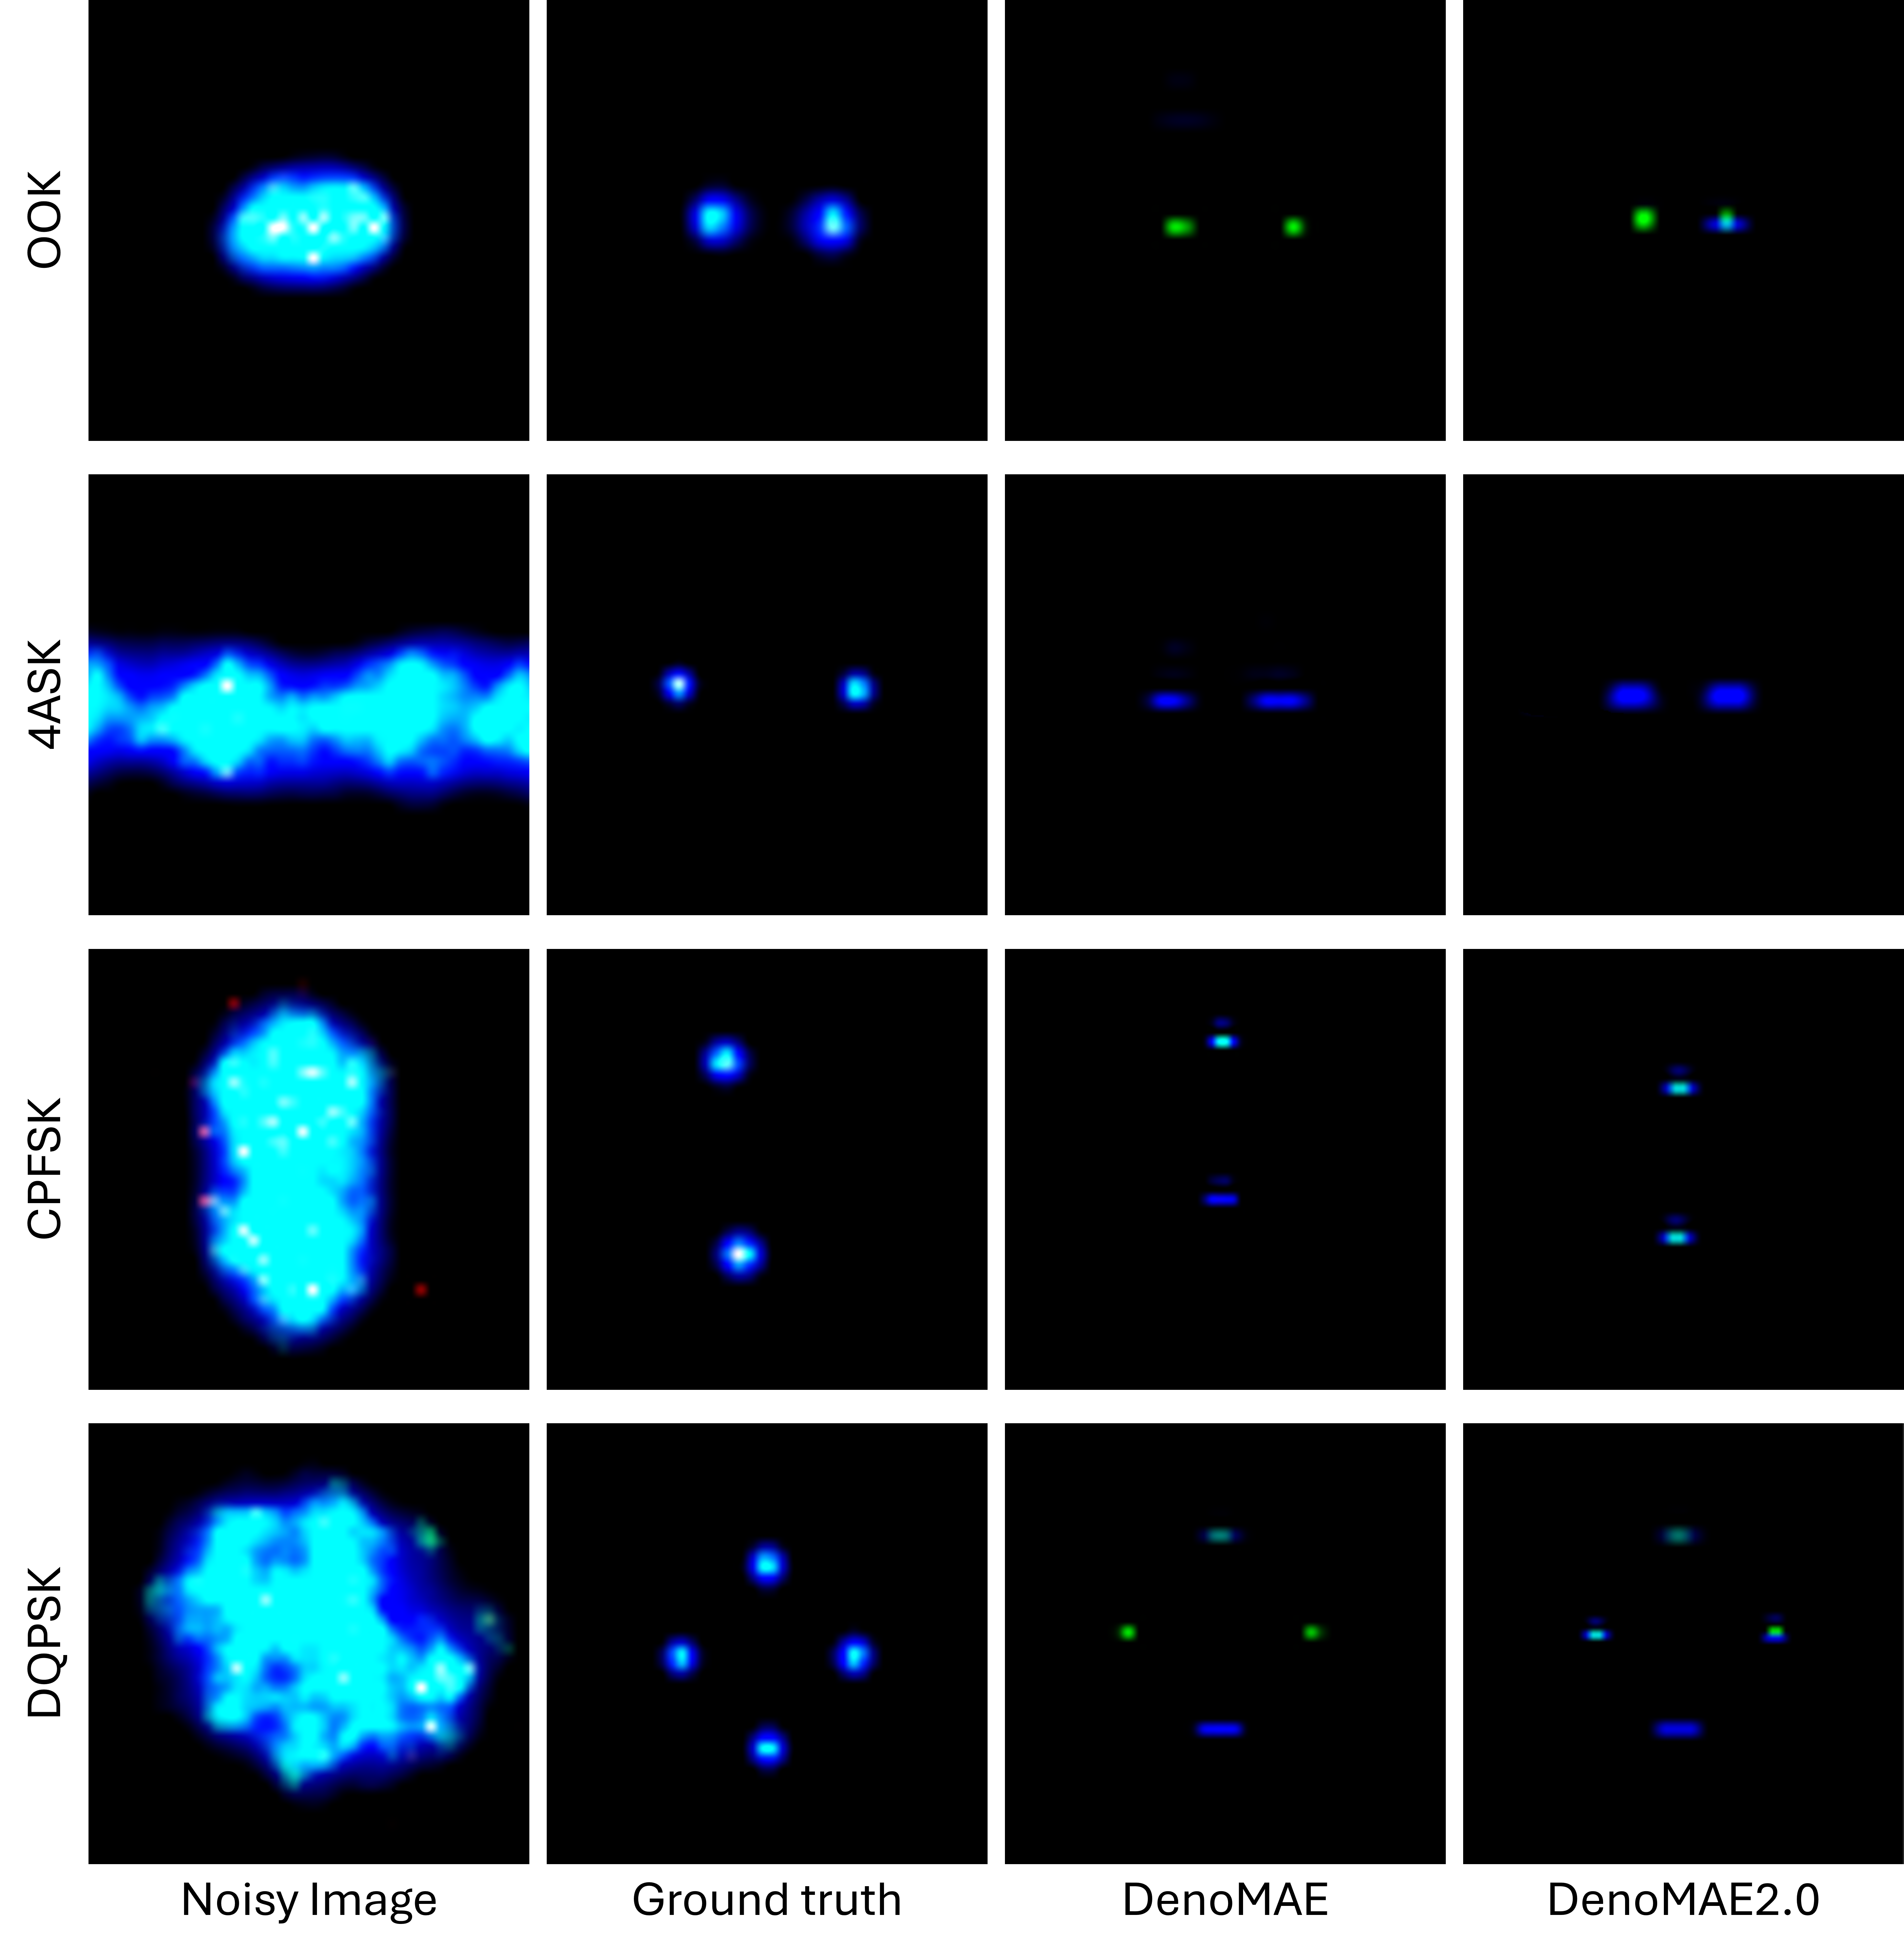
\includegraphics[width=0.9\linewidth]{FIGURES/denomae2/recon.png}
%     \caption{Reconstruction performance comparison between DenoMAE and DenoMAE2.0}
%     \label{fig:recon}
% \end{figure}

% During the pretraining phase, DenoMAE2.0 learns to denoise and reconstruct missing patches, thereby developing robust signal representations. We evaluate this denoising and reconstruction performance both during and after pretraining. Figure \ref{fig:recon} illustrates the effectiveness of DenoMAE2.0 through reconstructed constellation diagrams compared to the original DenoMAE model. DenoMAE2.0 achieves superior noise reduction while preserving critical signal features necessary for accurate modulation classification.

% Table \ref{tab:ssim_psnr_comparison} quantifies these improvements using two standard image quality metrics: structural similarity index (SSIM) and peak signal-to-noise ratio (PSNR). We report the mean SSIM and PSNR scores across all validation images (ten images per class) during pretraining. The results demonstrate that DenoMAE2.0 consistently outperforms the original DenoMAE across all modulation classes. For SSIM, DenoMAE2.0 shows improvements ranging from minor enhancements (0.0004 increase for DQPSK) to substantial gains (0.0315 increase for 4PAM). Similarly, for PSNR, DenoMAE2.0 achieves consistent improvements across all classes, with particularly notable enhancements for GMSK (0.2793 dB increase) and OOK (0.2911 dB increase). These consistent improvements in reconstruction quality metrics directly contribute to the enhanced downstream classification performance of DenoMAE2.0.

% \begin{table*}[htbp]
%     \centering
%     \caption{Quantitative Comparison of Denoising Performance between DenoMAE and DenoMAE2.0.}
%     \label{tab:ssim_psnr_comparison}
%     \renewcommand{\arraystretch}{1.1}
%     \begin{tabular}{ccccc}
%         \hline
%         \multirow{2}{*}{\textbf{Class}} & \multicolumn{2}{c}{\textbf{SSIM}} 
%         & \multicolumn{2}{c}{\textbf{PSNR}} \\ 
%         \cline{2-3} \cline{4-5}
%         & \textbf{DenoMAE} & \textbf{DenoMAE2.0} & \textbf{DenoMAE} & \textbf{DenoMAE2.0} \\ \hline
%         16PAM  & 0.9422 & 0.9464 & 41.6867 & 41.8003 \\
%         4ASK   & 0.9607 & 0.9634 & 42.1780 & 42.3096 \\
%         4PAM   & 0.9328 & 0.9643 & 42.0005 & 42.1061 \\
%         8ASK   & 0.9745 & 0.9813 & 42.8006 & 42.9158 \\
%         CPFSK  & 0.9719 & 0.9738 & 42.3492 & 42.5520 \\
%         DQPSK  & 0.9356 & 0.9360 & 41.8405 & 41.9223 \\
%         GFSK   & 0.9677 & 0.9681 & 42.0733 & 42.1021 \\
%         GMSK   & 0.8749 & 0.8771 & 39.9367 & 40.2160 \\
%         OOK    & 0.9586 & 0.9674 & 42.3674 & 42.6585 \\
%         OQPSK  & 0.9129 & 0.9204 & 41.0052 & 41.1172 \\ \hline
%     \end{tabular}
% \end{table*}

% \subsubsection{Latent Space Visualization with TSNE}

% In Figure~\ref{fig:tsne}, we visualize the latent representations of DenoMAE and DenoMAE2.0 using t-distributed stochastic neighbor embedding (t-SNE)~\cite{van2008visualizing}. The plots (left two) reveal that DenoMAE2.0 produces more accurate and distinct clusters than DenoMAE, indicating superior feature separation and representation learning. Specifically, in DenoMAE, classes 0, 3, and 9 contain more separated clusters within the same class. In contrast, DenoMAE2.0 exhibits more distinct clusters for these classes.

% This enhanced clustering is particularly evident in the masked samples (right two plots), where we mask out a significant portion (75\%) of the images. Masking typically makes distinct cluster formation more challenging. However, DenoMAE2.0 achieves clearer boundaries between classes, suggesting improved robustness and generalization capabilities. In DenoMAE, classes 0, 3, and 9 achieve somewhat distinct clusters, with a few samples overlapping in other clusters. In DenoMAE2.0, classes 0, 3, 6, 7, 8, and 9 show better-separated clusters, indicating enhanced feature learning and representation.

% However, in all the plots, classes 1 and 2 entirely overlap with each other, indicating that the model struggles to distinguish between these two classes. This is a common issue in modulation classification, as some classes are very similar to each other.

% \begin{figure*}
%     \centering
%     \subfloat{%
%        \includegraphics[trim=1cm 1cm 1cm 1cm,clip,
%        width=0.25\linewidth]{FIGURES/denomae2/denoMAE_no_mask.png}}
%     \hfill
%     \subfloat{%
%         \includegraphics[trim=1cm 1cm 1cm 1cm,clip,
%         width=0.25\linewidth]{FIGURES/denomae2/denoMAE2_no_mask.png}}
%     \hfill
%     \subfloat{%
%         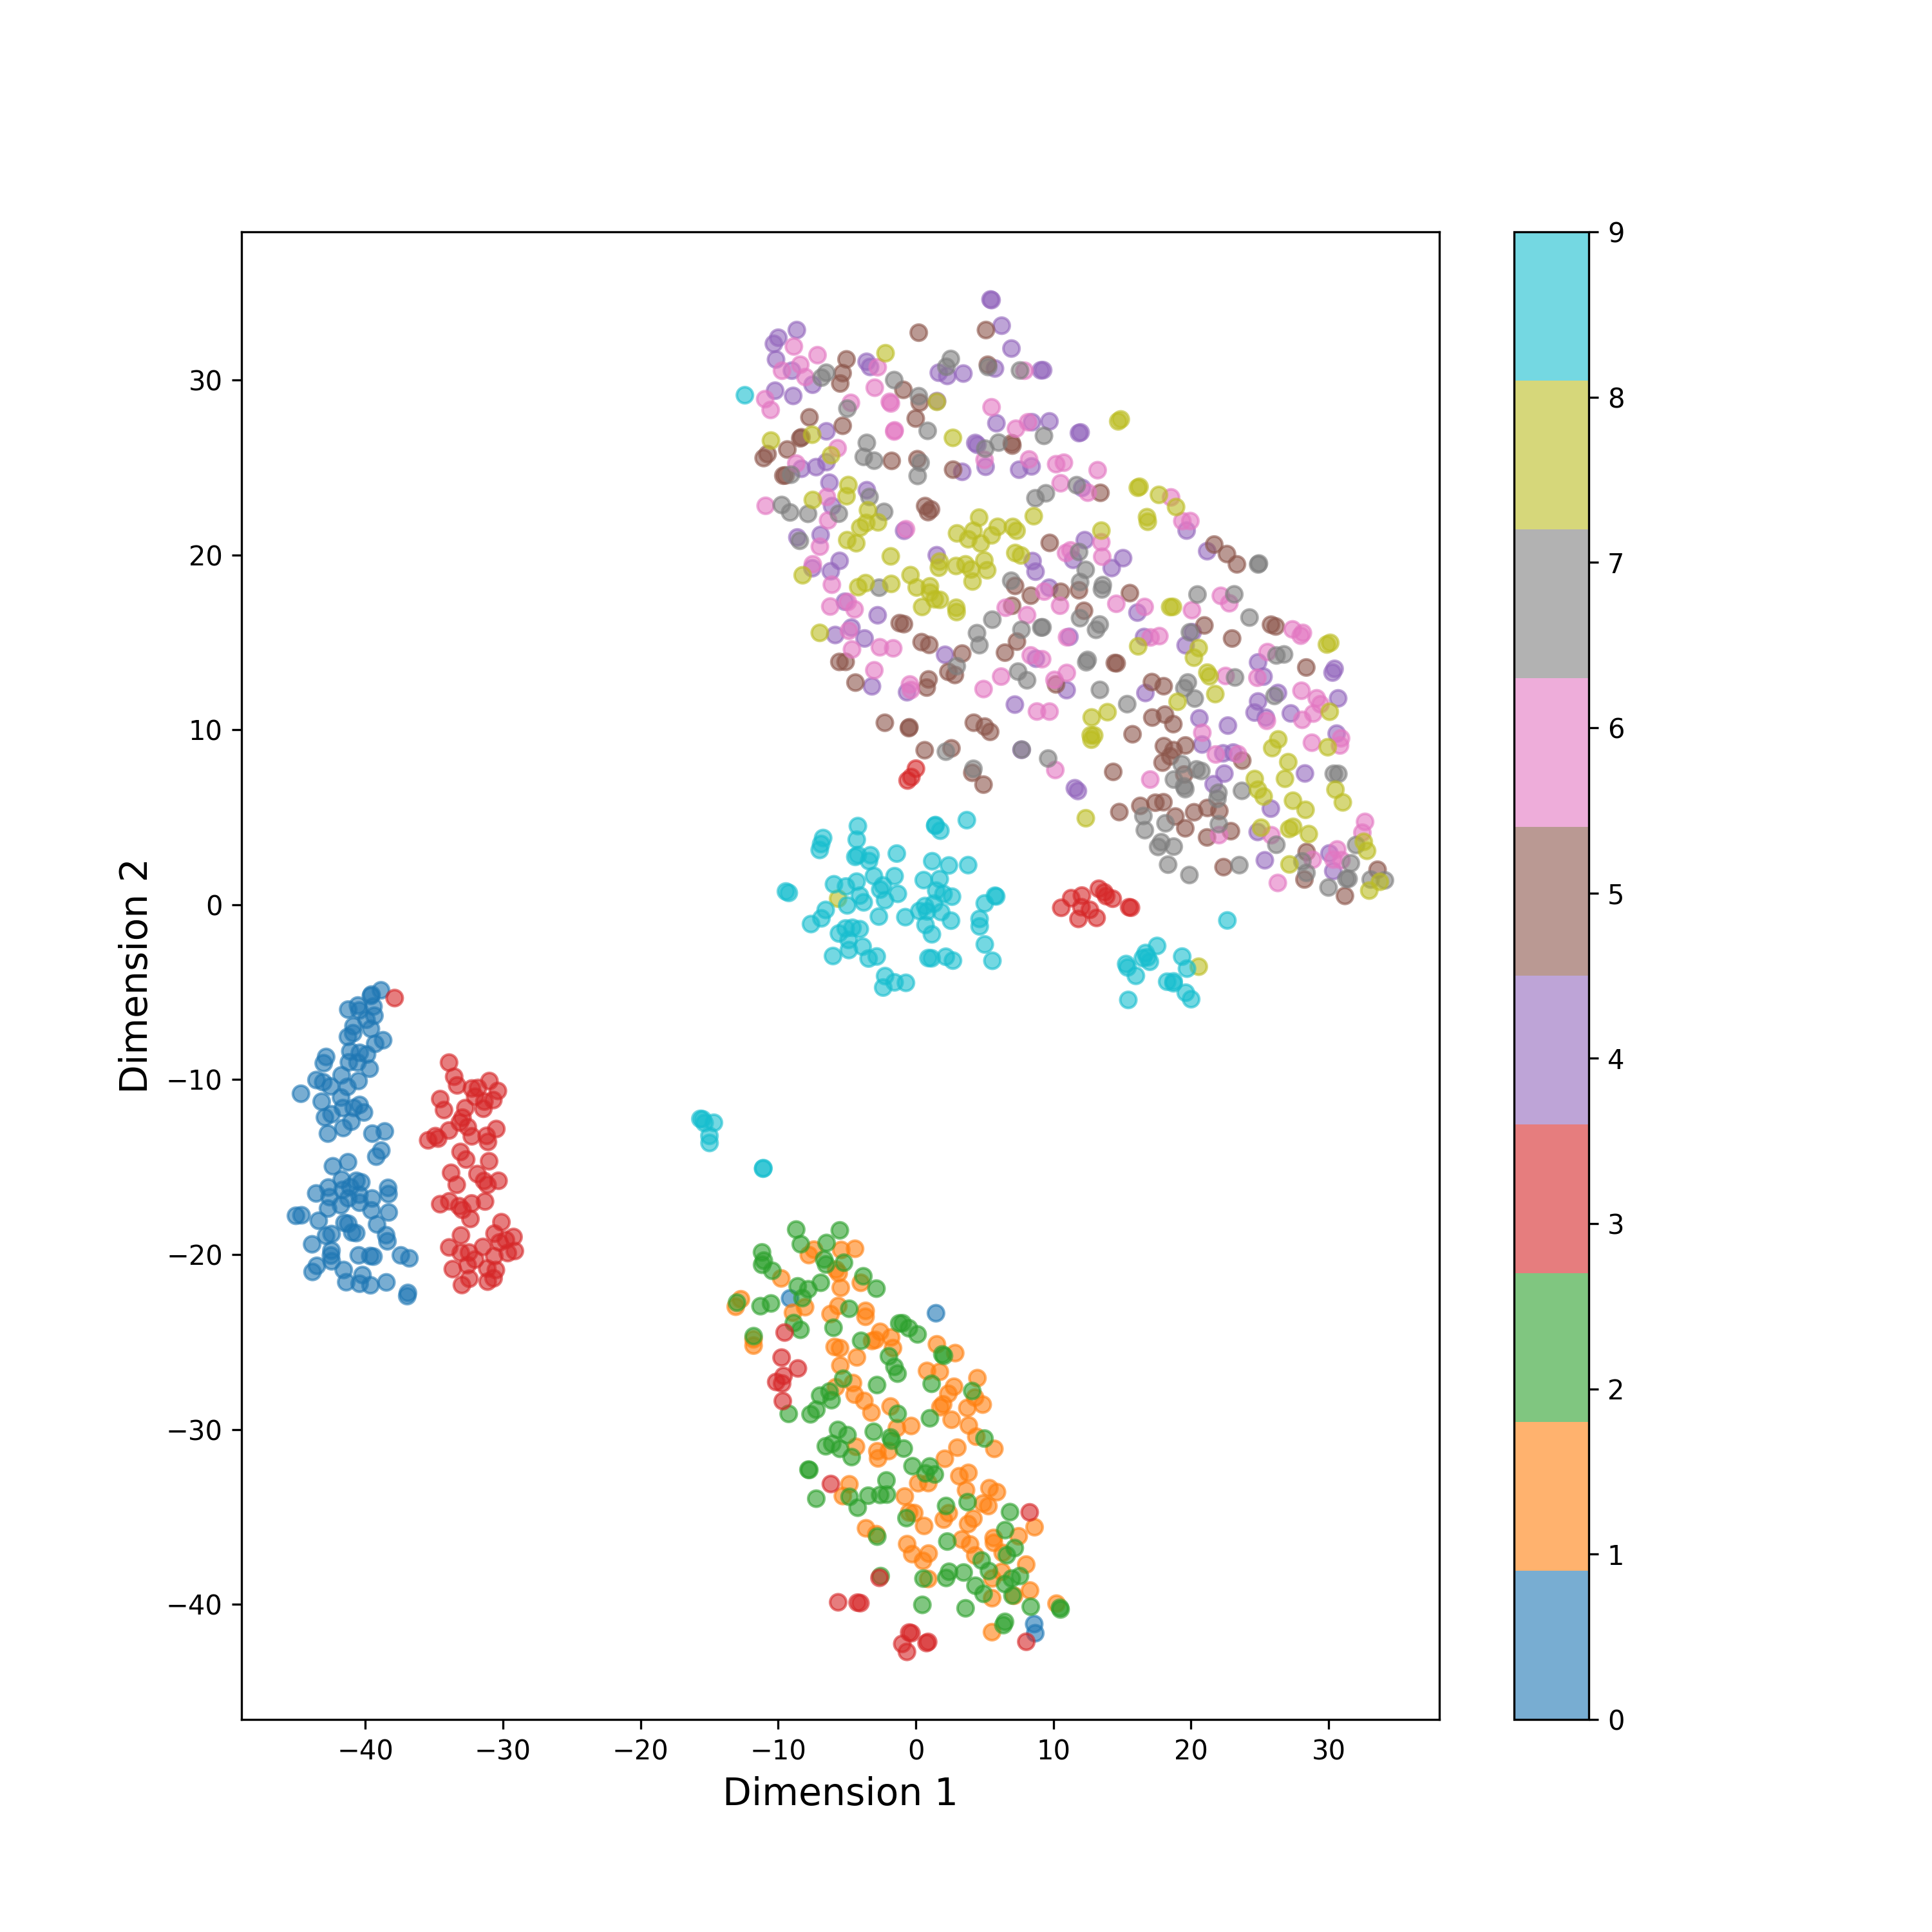
\includegraphics[trim=1cm 1cm 1cm 1cm,clip,
%         width=0.25\linewidth]{FIGURES/denomae2/denoMAE_mask.png}}
%     \hfill
%     \subfloat{%
%         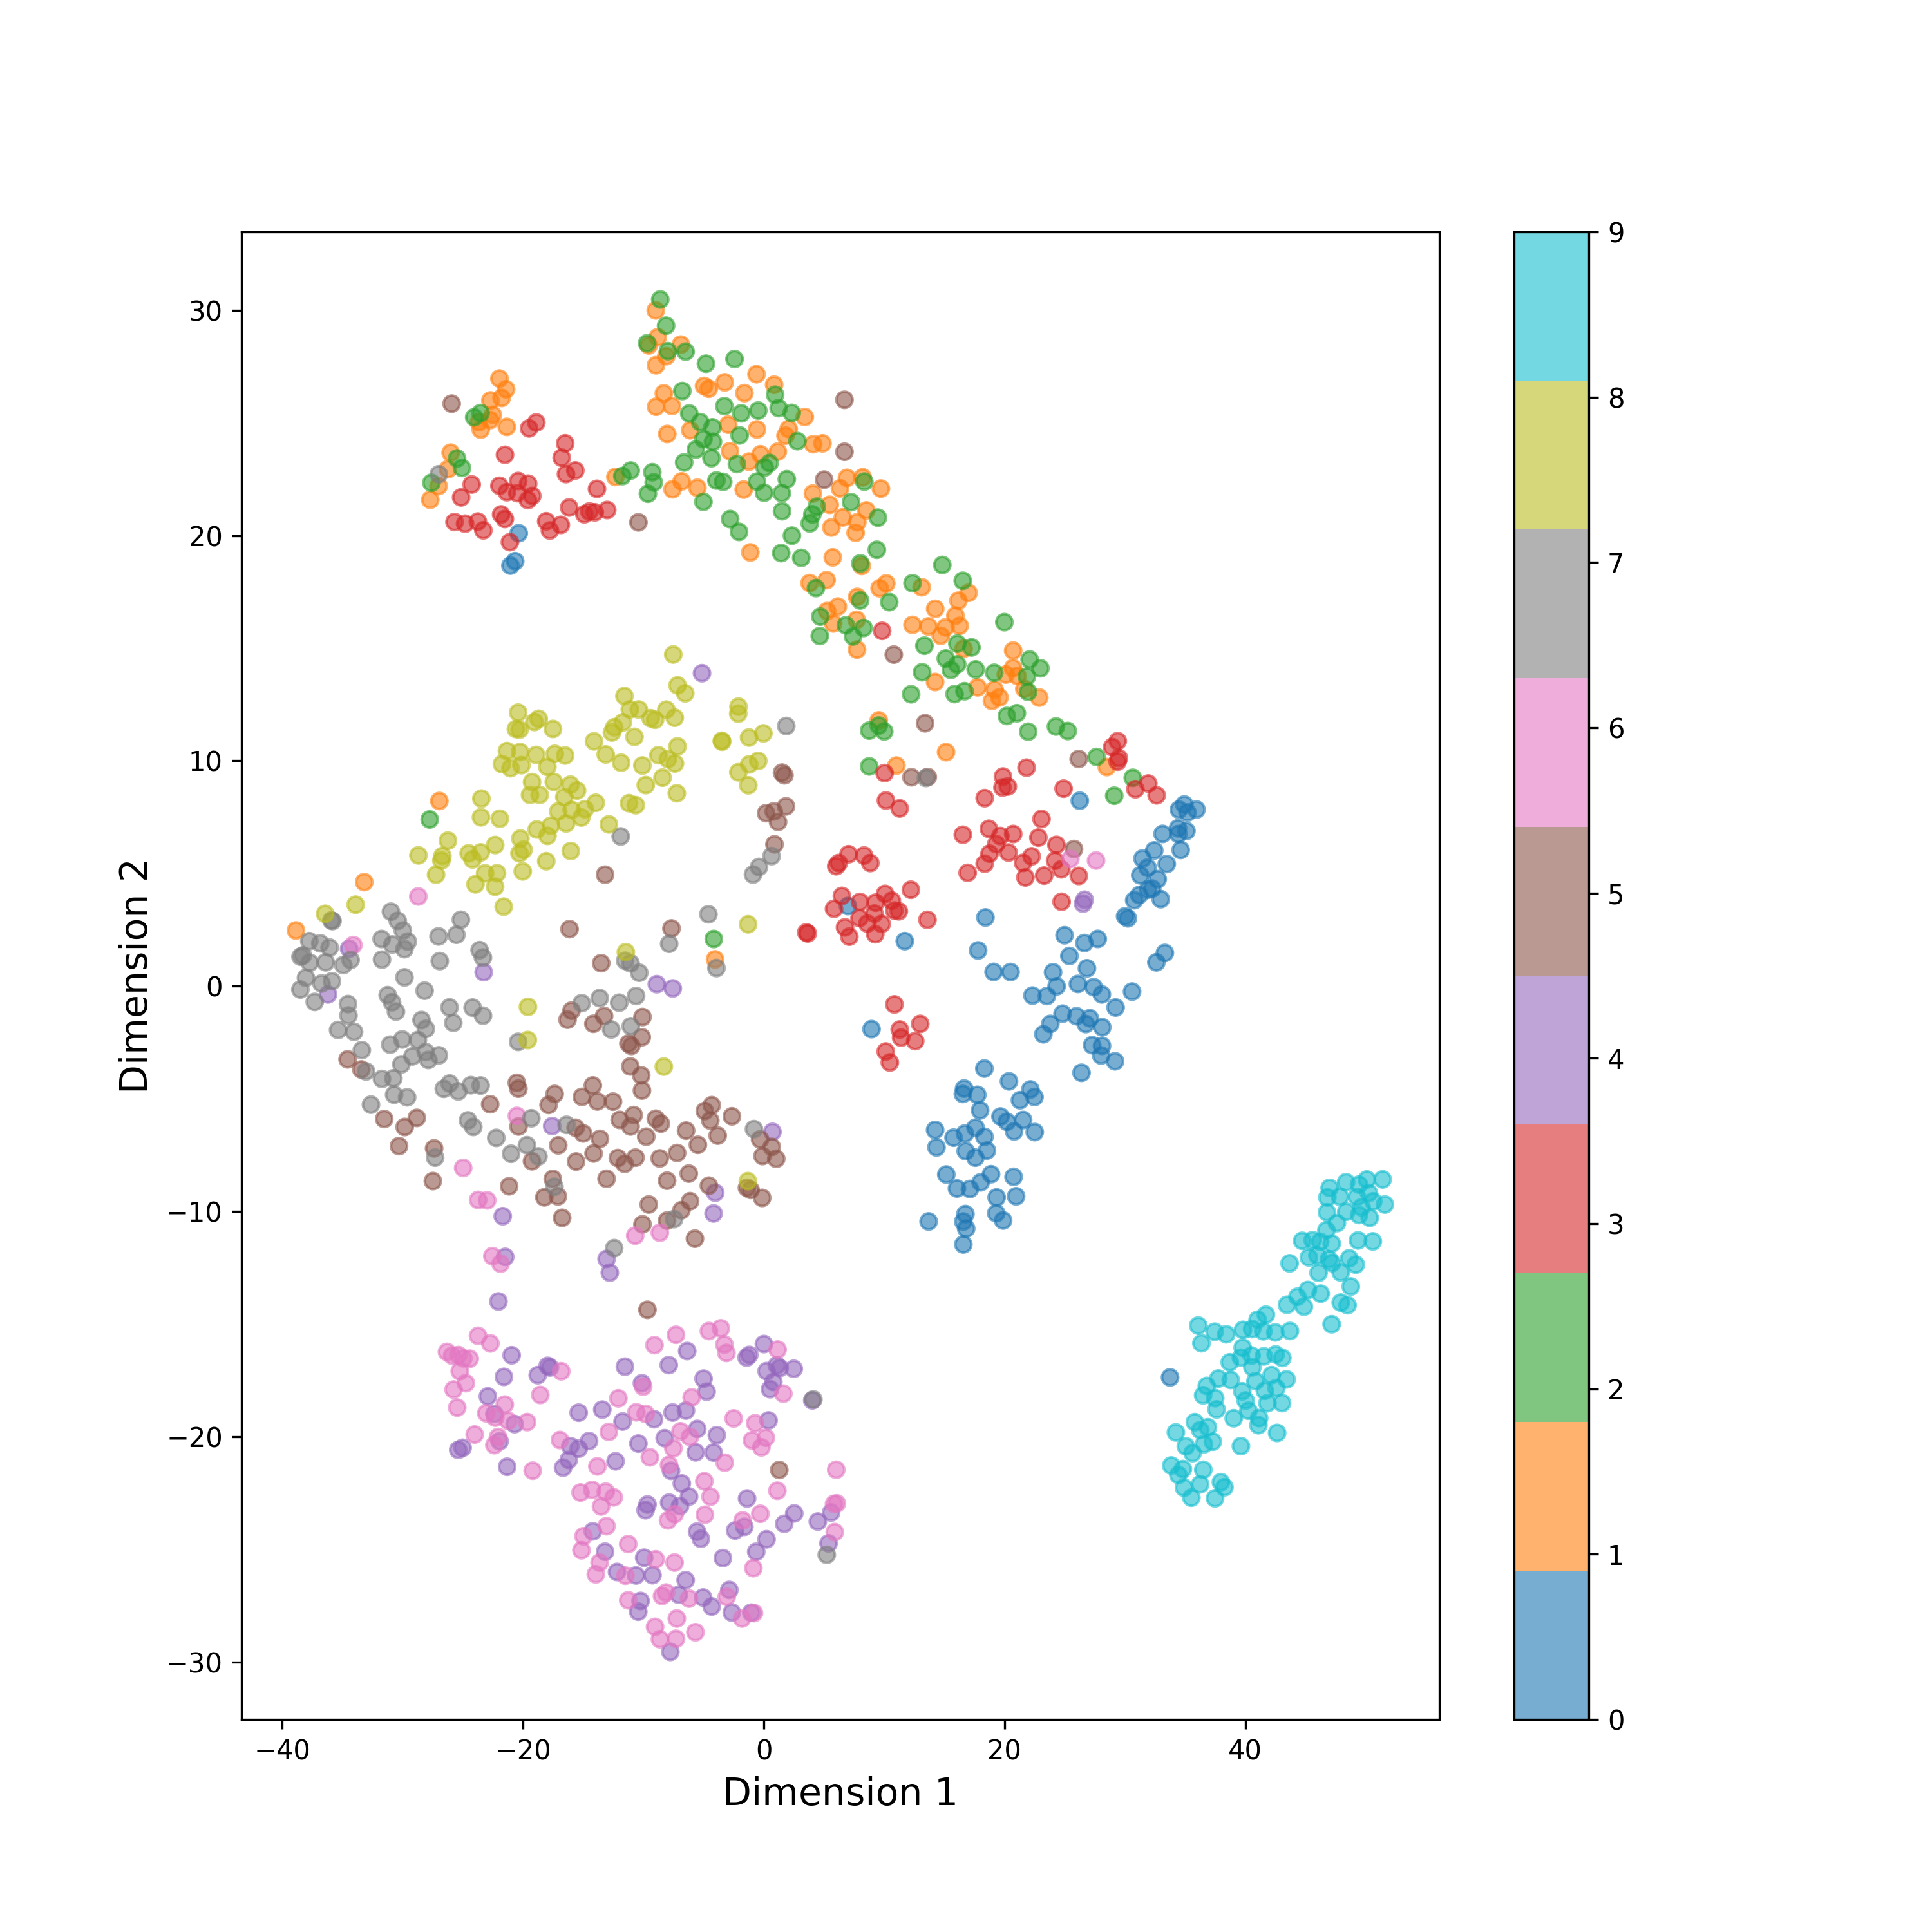
\includegraphics[trim=1cm 1cm 1cm 1cm,clip,
%         width=0.25\linewidth]{FIGURES/denomae2/denoMAE2_mask.png}}
%     \caption{Latent representation visualization using t-SNE. From left to right: (1) DenoMAE without masking, (2) DenoMAE2.0 without masking, (3) DenoMAE with 75\% masking, and (4) DenoMAE2.0 with 75\% masking.}
%     \label{fig:tsne} 
% \end{figure*}

% \subsubsection{Finetuning Accuracy}

% After pretraining, we transfer the learned representations to the downstream classification task and compare DenoMAE2.0 with state-of-the-art models. As shown in Table \ref{tab:example}, when finetuned on the downstream task, DenoMAE2.0 achieves the highest test accuracy of 82.40\% among all compared methods. This represents a significant improvement over the baseline ViT (79.90\%) and other representation learning approaches including DEiT (81.20\%), MoCov3 (81.00\%), BEiT (80.40\%), MAE (80.10\%), and the original DenoMAE (81.30\%). The consistent performance advantage demonstrates that DenoMAE2.0's enhanced denoising strategy learns more effective representations during pretraining that transfers well to the downstream classification task.

% \begin{table}[htbp]
%     \centering
%     \caption{Downstream classification accuracy for different models}
%     \begin{tabular}{cc}
%         \hline
%         \textbf{Method} & \textbf{Test accuracy (\%)} \\ \hline
%         ViT \cite{dosovitskiy2020image} & 79.90 \\ 
%         DEiT \cite{touvron2021training} & 81.20 \\ 
%         MoCov3 \cite{xie2021self} & 81.00 \\ 
%         BEiT \cite{bao2021beit} & 80.40 \\
%         MAE \cite{he2022masked} &  80.10 \\ 
%         DenoMAE \cite{faysal2025denomae} &  81.30 \\
%         DenoMAE2.0  (\textbf{Ours}) &  \textbf{82.40} \\ \hline
%     \end{tabular}
%     \label{tab:example}
% \end{table}

% \subsubsection{Confusion Matrix}

% Figure~\ref{fig:confusion} presents confusion matrices visualizing the per-class performance of both DenoMAE and DenoMAE2.0. The diagonal elements indicate correct classifications, while off-diagonal elements show misclassifications. Both models demonstrate perfect classification accuracy (100\%) for several modulation types, specifically 16PAM, 4ASK, 8ASK, DQPSK, GMSK, OOK, and OQPSK. 

% However, persistent classification challenges are evident between 4ASK and 4PAM, where both models show significant confusion with 50\% accuracy for each class and 50\% misclassification between them. This symmetric confusion pattern suggests inherent signal similarities between these amplitude modulation schemes that remain difficult to distinguish even with our enhanced architecture. Notably, this confusion pattern directly aligns with observations from the t-SNE analysis, where classes 1 and 2 show complete overlap in the latent space visualization, further confirming the inherent similarity in signal characteristics between these modulation types.

% Additionally, both models struggle with differentiating between CPFSK and GFSK, though DenoMAE2.0 shows modest improvement in CPFSK recognition (70\% accuracy compared to 63\% in DenoMAE). Despite this improvement, GFSK classification remains challenging with DenoMAE2.0 achieving only 54\% accuracy (compared to 52\% in DenoMAE), with most misclassifications assigning GFSK signals to the CPFSK class. This confusion pattern aligns with the theoretical similarity between these frequency shift keying techniques, as GFSK is essentially CPFSK with additional Gaussian filtering. These consistent patterns across both model versions indicate fundamental signal similarities that present intrinsic classification challenges rather than model limitations.

% \begin{figure}[htbp]
%     \centering
%     \subfloat{%
%         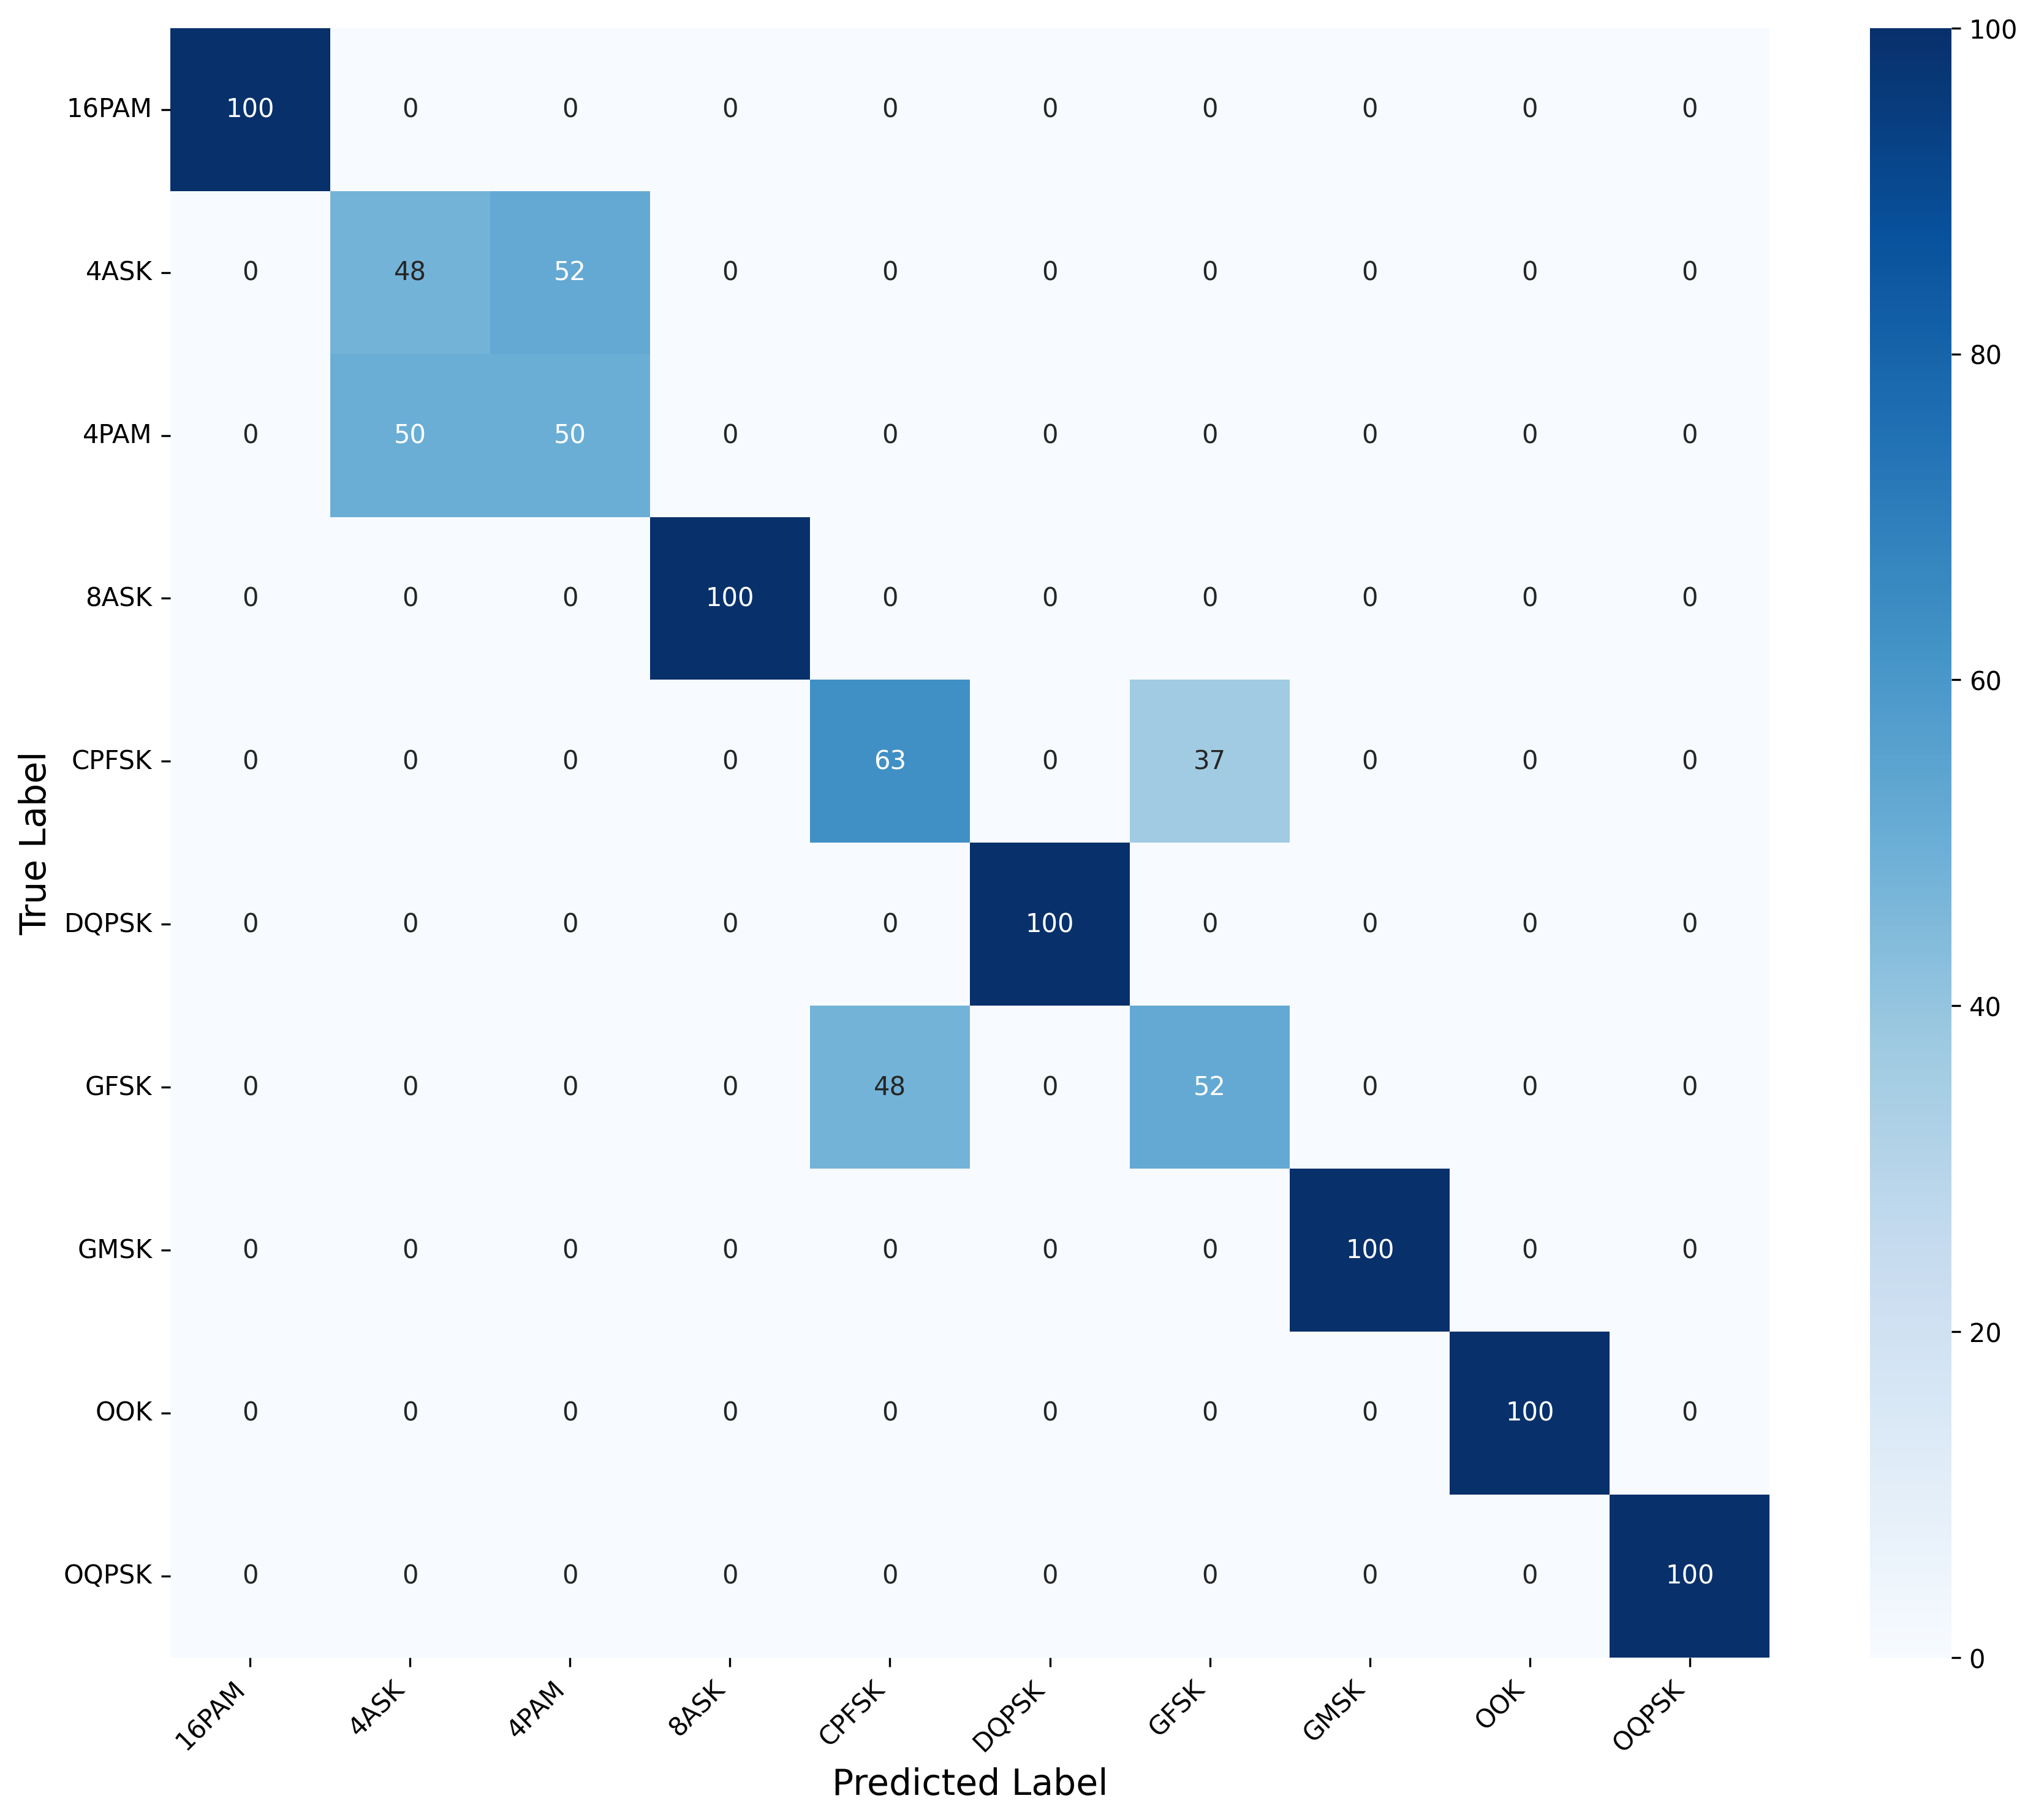
\includegraphics[width=0.48\linewidth]{FIGURES/denomae2/deno_cm.png}}
%     \hfill
%     \subfloat{%
%         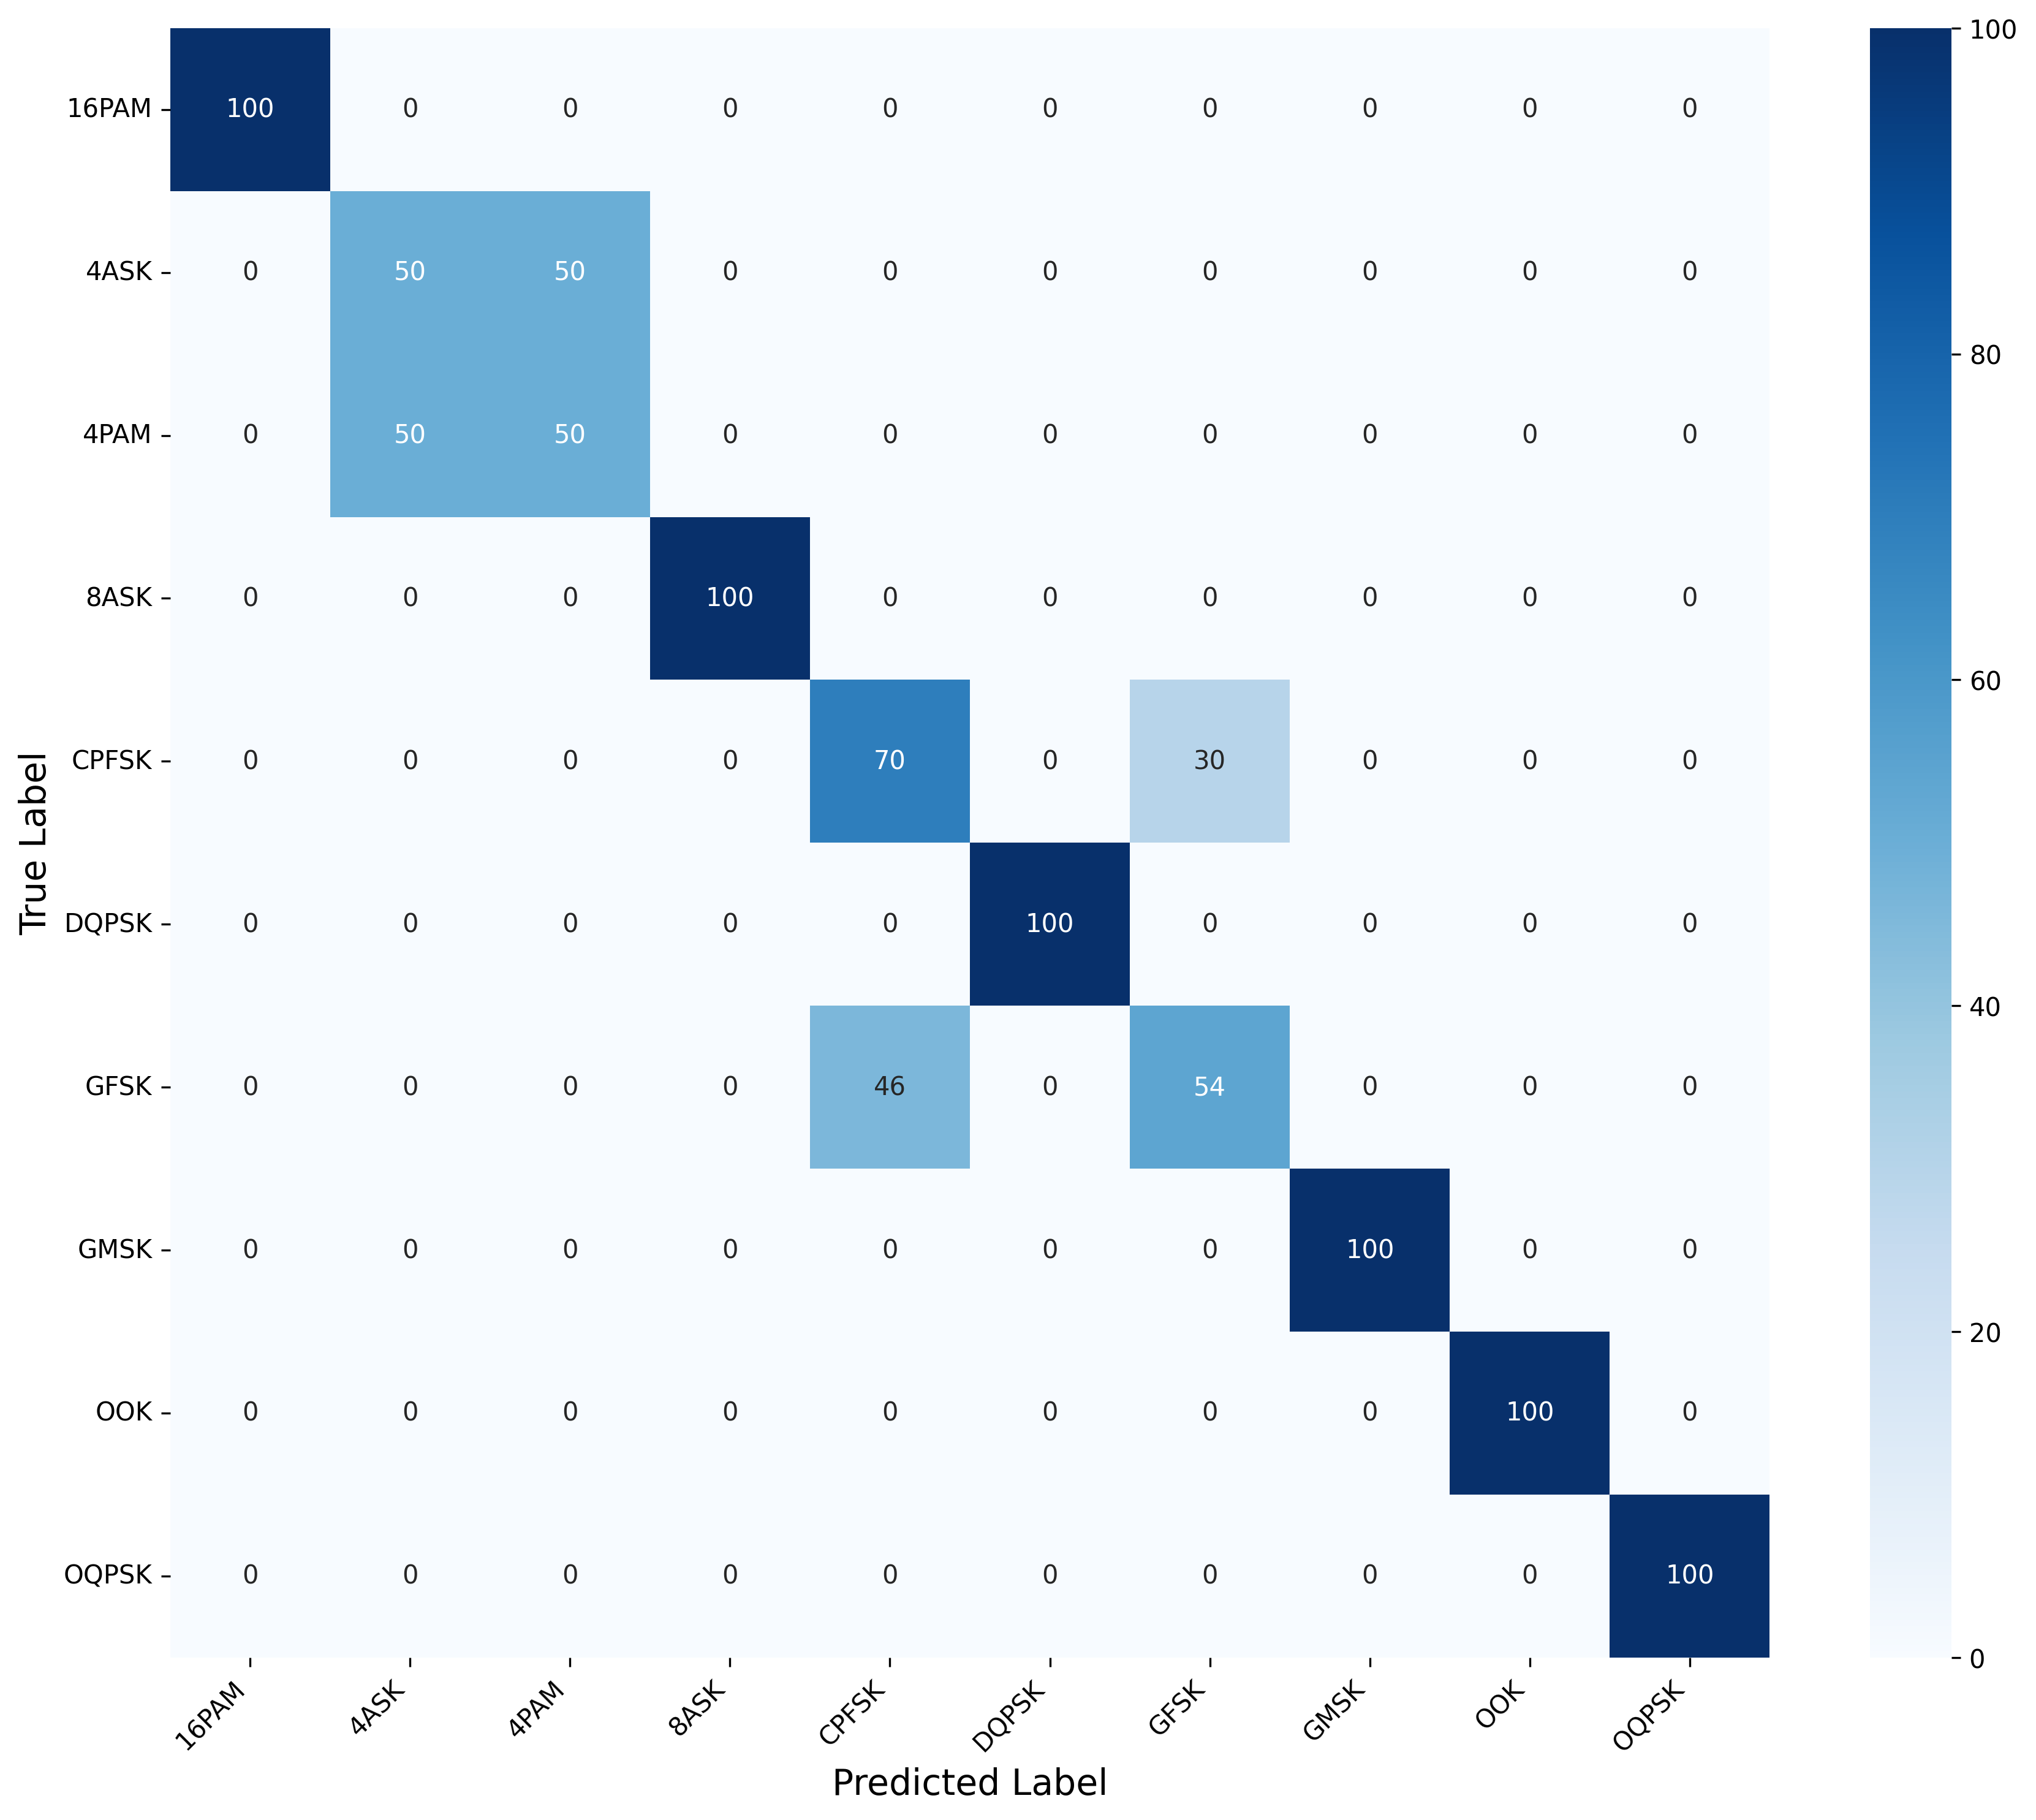
\includegraphics[width=0.48\linewidth]{FIGURES/denomae2/deno2_cm.png}}
%     \caption{Confusion matrices for downstream classification. Left: DenoMAE, Right: DenoMAE2.0} 
%     \label{fig:confusion}
% \end{figure}


% \subsubsection{Performance on Number of Epochs}

% \begin{figure}[htbp]
%     \centering
%     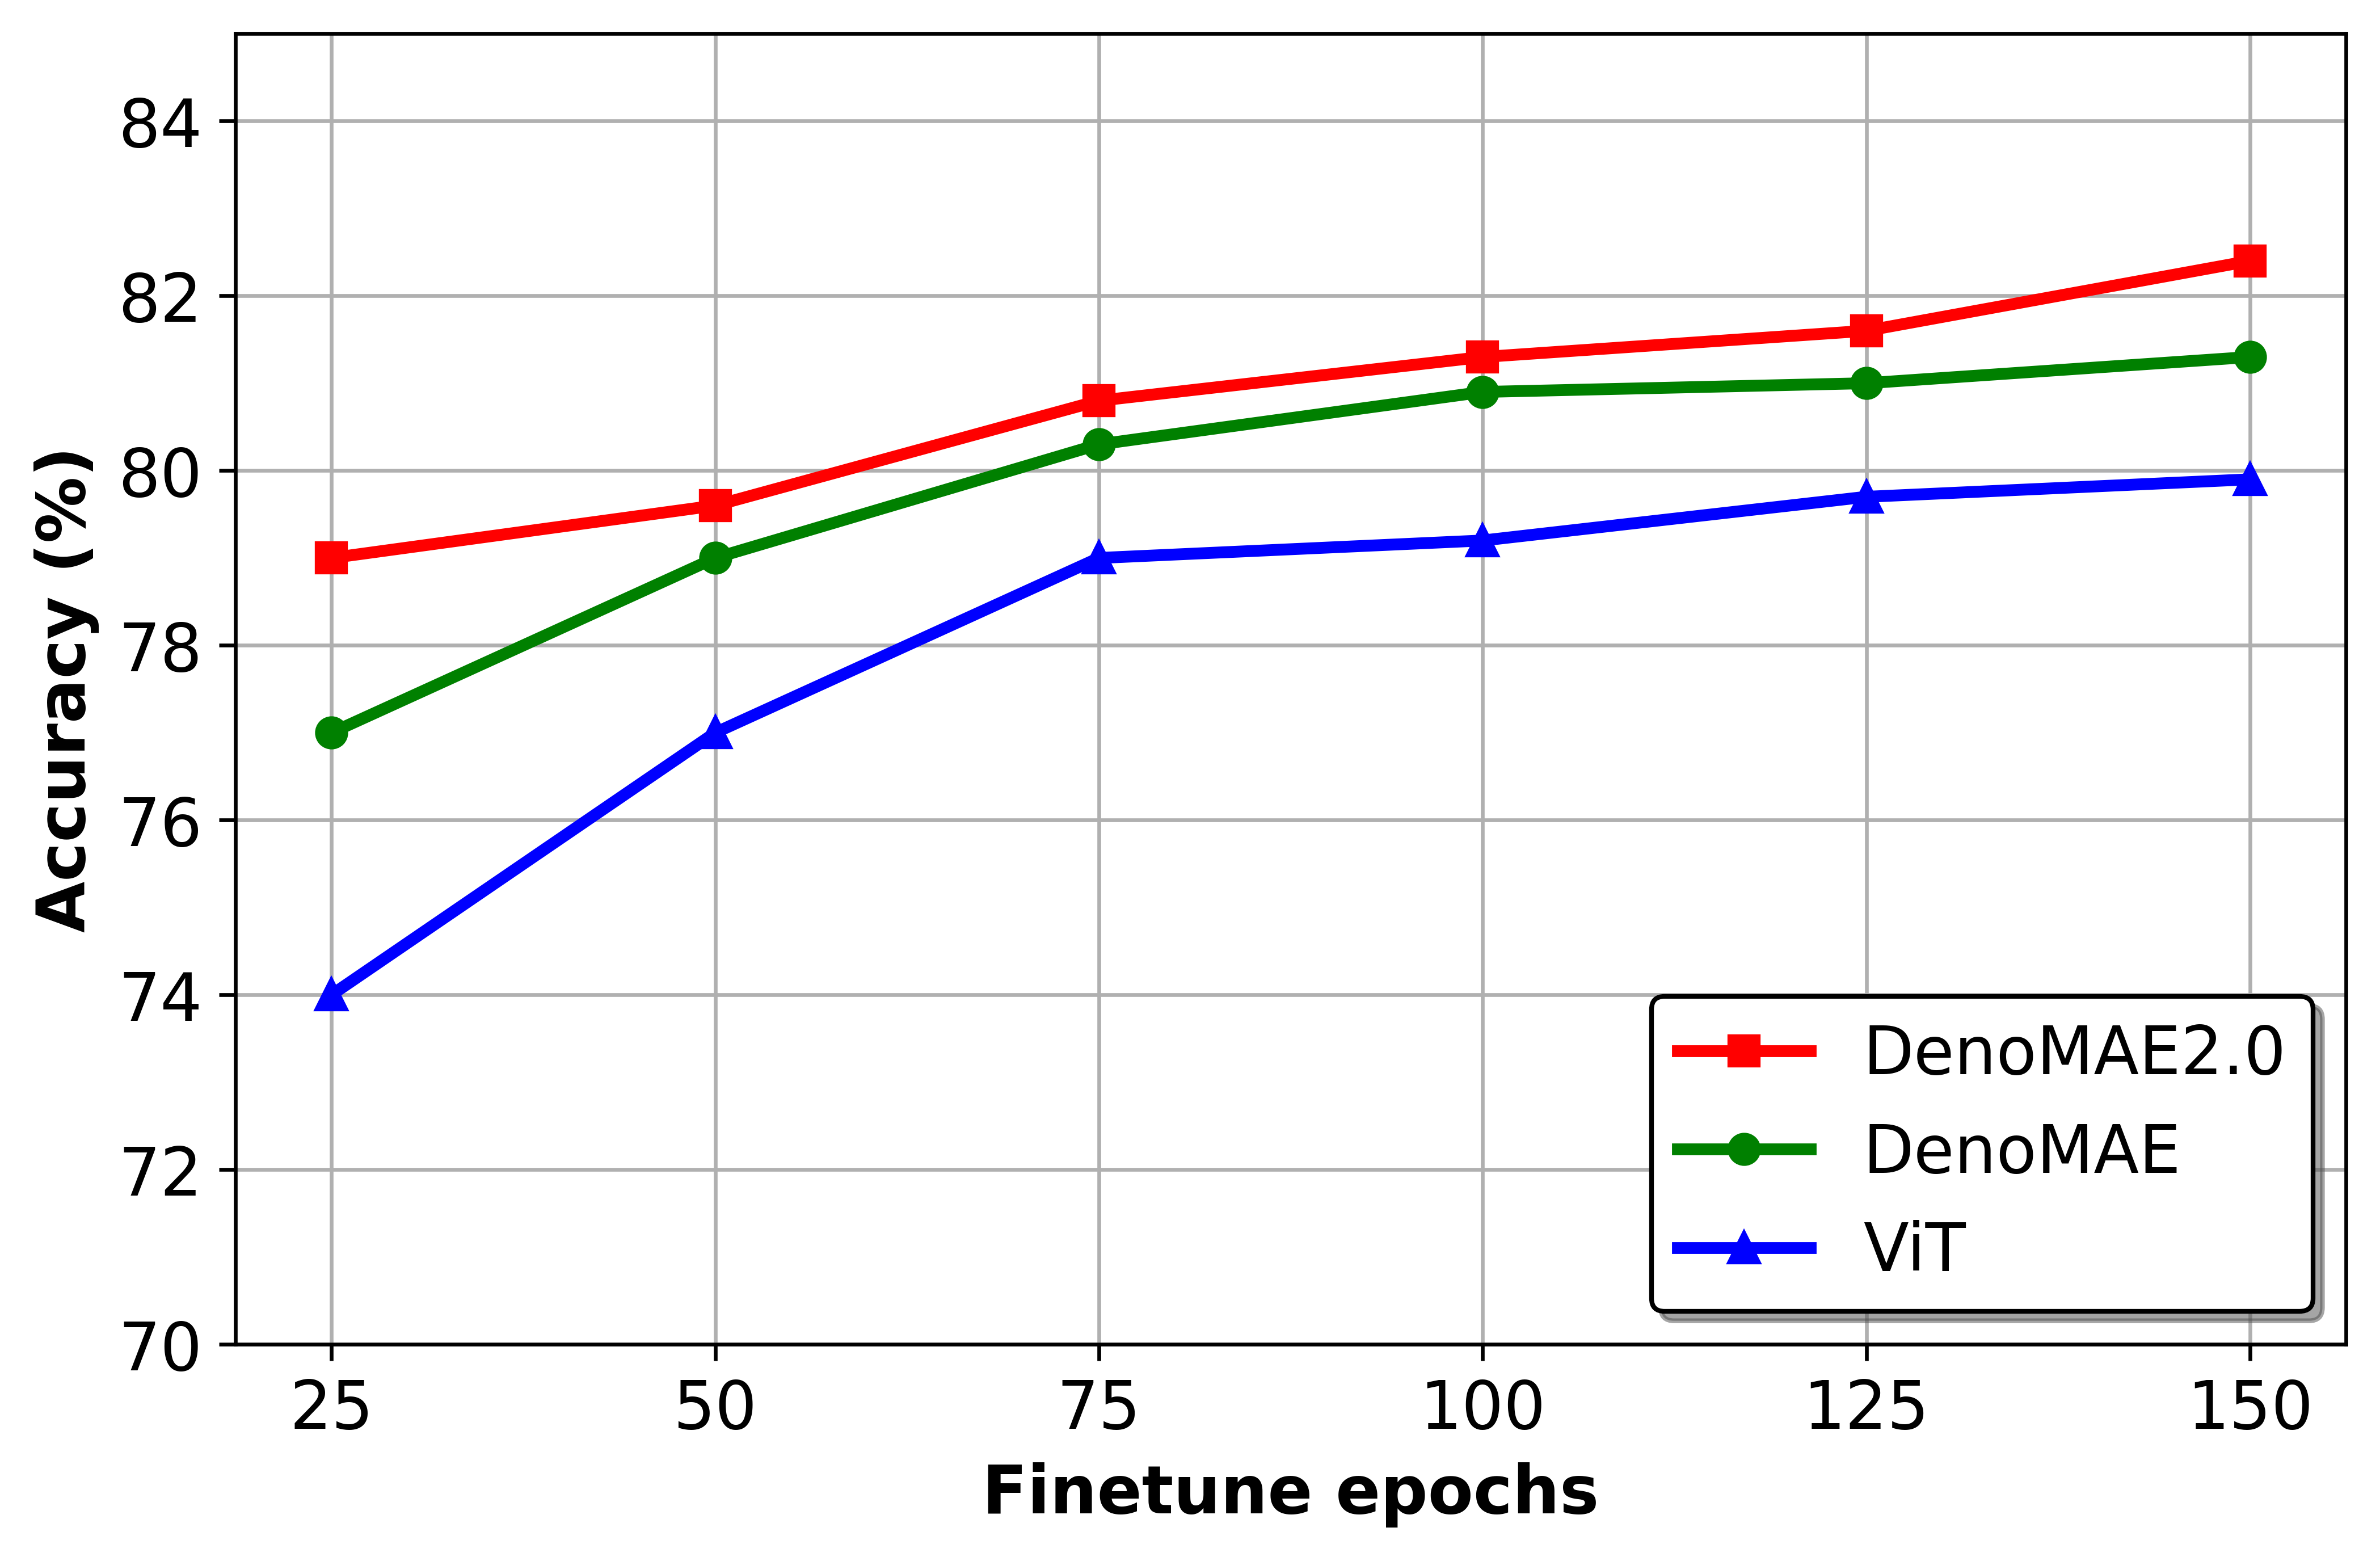
\includegraphics[width=0.9\linewidth]{FIGURES/denomae2/finetune_epoch.png}
%     \caption{Finetuning performance improvement for  different epochs}
%     \label{fig:epoch}
% \end{figure}

% Figure~\ref{fig:epoch} illustrates the finetuning performance across different epochs. The plot shows a steady improvement in model accuracy as the number of epochs increases, with DenoMAE2.0 consistently outperforming baseline methods. DenoMAE achieves higher accuracy than ViT continuously. On the other hand, although the gap between DenoMAE and ViT is larger than DenoMAE and DenoMAE2.0, DenoMAE2.0 always obtains better accuracy than DenoMAE.

% \subsubsection{Performance Across Different SNRs}

% The SNR performance plot demonstrates robust classification accuracy across various SNRs ranging from -10 dB to 10 dB. As the SNR values increases all the methods perform better and when the SNR is low the performance degrades. ViT, which has no pertaining phase, presumably obntains the lowest performance in all cases. MAE, which pretrains on modulation signals but has no denoising capability, obtains a slight higher accuracy than ViT. DenoMAE obtains higher accuracy than MAE in most cases however for SNE of 2 and 3 we observe that MAE obtains a higher accuracy. On the other hand, DenoMAE2.0 outperforms all the methods for all the SNRs.  Noteably, all the methods lose significant accuracy for snr lower than -2 dB. However, DenoMAE2.0 maintains comparatively robust performance down to -7 dB, demonstrating its enhanced resilience to noise.

% \begin{figure}[htbp]
%     \centering
%     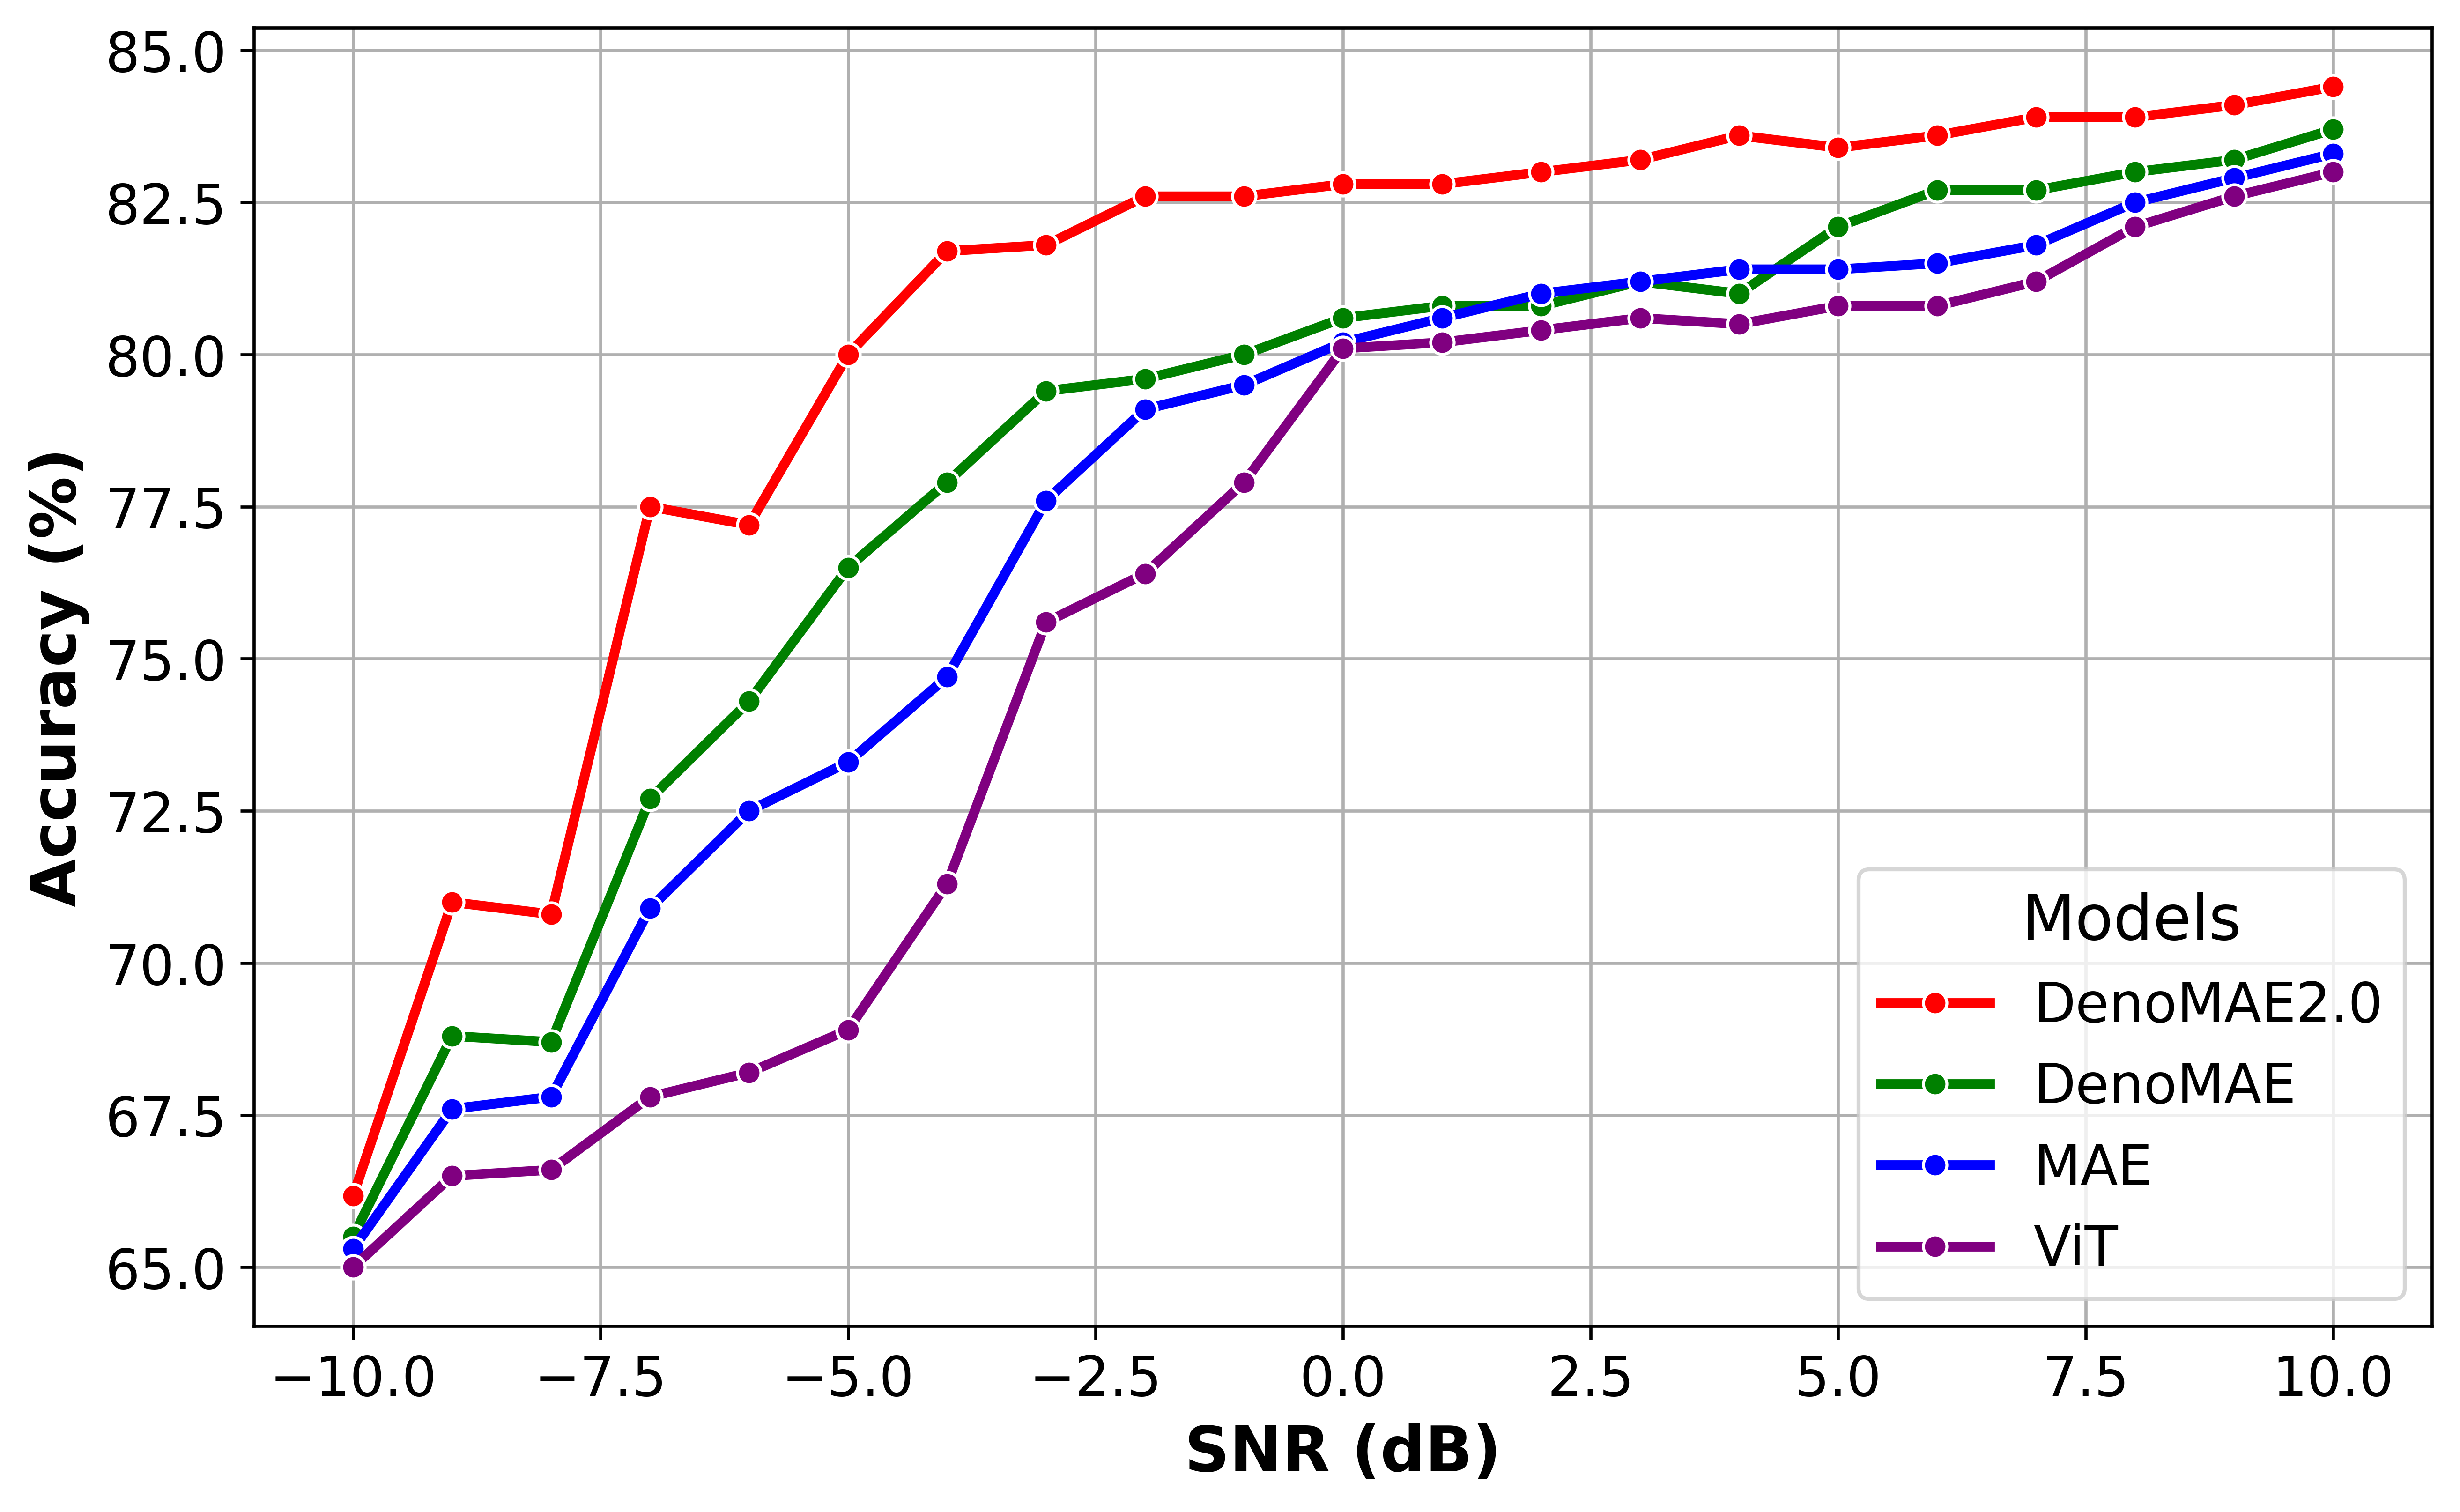
\includegraphics[width=\linewidth]{FIGURES/denomae2/SNR_Accuracy_Plot.png}
%     \caption{Accuracy comparison across different SNRs}
%     \label{fig:snr_acc}
% \end{figure}

% \subsection{Comparison with Other AMC Methods}

% Table~\ref{tab:compare} presents a comprehensive comparison between DenoMAE2.0 and other state-of-the-art modulation classification methods. AlexNet achieved 82.8\% accuracy with 8 classes at 2dB SNR using a large dataset of 800,000 samples. NMformer reported 71.6\% accuracy across 10 classes with SNR ranging from 0.5 to 4.5dB using 106,800 samples. CNN-AMC and DL-GRF showed relatively lower performance with 50.40\% and 59\% accuracy respectively, though they were tested under different conditions. The original DenoMAE achieved 81.3\% accuracy across 10 classes with SNR ranging from 0 to 10dB. Our proposed DenoMAE2.0 demonstrates superior performance with 82.4\% accuracy under similar conditions, using only 10,000 samples for pretraining and 1,000 samples for fine-tuning, indicating improved efficiency in both performance and data utilization.

% \begin{table}[htbp]
%     \centering
%     \caption{Comparison of DenoMAE2.0 with other modulation classification methods}
%     \label{tab:compare}
%     \begin{tabular}{cccccc}
%     \toprule
%     \multirow{2}{*}{\textbf{Methods}} & \multicolumn{2}{c}{\textbf{Number of samples}} & \multirow{2}{*}{\textbf{SNR (dB)}} & \multirow{2}{*}{\textbf{\# Classes}} & \multirow{2}{*}{\textbf{Accuracy (\%)}} \\ 
%     \cmidrule(lr){2-3}
%      & \textbf{Pretraining} & \textbf{Fine-tuning} & & \\ \midrule
    
%     AlexNet \cite{peng2018modulation}     & 800,000 (train) & 8,000 (test)   & 2         & 8  & 82.8  \\
%     NMformer \cite{faysal2024nmformer}    & 106,800         & 3,000          & 0.5–4.5   & 10 & 71.6  \\
%     CNN-AMC \cite{meng2018automatic}      & 79,200          & 228,060        & –6        & 4  & 50.4  \\
%     DL-GRF \cite{sun2022automatic}        & 2,000 (train)   & 200 (test)     & 0         & 4  & 59    \\
%     DenoMAE \cite{faysal2025denomae}      & 10,000          & 1,000          & 0–10      & 10 & 81.3  \\
%     \textbf{DenoMAE2.0 (Ours)}            & 10,000          & 1,000          & 0–10      & 10 & \textbf{82.4} \\
    
%     \bottomrule
%     \end{tabular}
% \end{table}

% \subsection{Ablation Study}

% In this section, we analyze the impact of various components on the performance of our model.

% \subsubsection{Effect of the Loss Function}

% We conducted experiments to evaluate the contribution of different loss components in our model. As shown in Table~\ref{tab:loss}, we analyzed three configurations: using only reconstruction loss, only classification loss, and combining both losses. The results demonstrate that while reconstruction loss alone achieves reasonable performance (81.30\%), classification loss by itself underperforms (69.80\%). However, combining both losses yields the best results (82.40\%), suggesting that the joint optimization of reconstruction and classification objectives leads to more robust feature learning and better overall performance.

% \begin{table}[htbp]
%     \centering
%     \caption{Accuracy for different loss configurations}
%     \begin{tabular}{ccc}
%         \toprule
%         Reconstruction Loss & Classification Loss & Accuracy (\%) \\
%         \midrule
%         \ding{51} &     & 81.30 \\
%                  & \ding{51} & 69.80 \\
%         \ding{51} & \ding{51} & 82.40 \\
%         \bottomrule
%     \end{tabular}
%     \label{tab:loss}
% \end{table}

% \subsubsection{Effect of Auxiliary Loss Weights}

% We conducted experiments to analyze the impact of auxiliary loss weights on model performance, as shown in Table~\ref{tab:weights_accuracy}. The results demonstrate that the model's accuracy varies with different weight values, with 0.10 achieving the optimal performance at 82.4\%. We observed a clear trend where very high weights (1.0) significantly degraded performance to 79.60\%, while moderate weights (0.25, 0.50) maintained consistent performance at 82.0\%. Lower weights (0.01, 0.05) showed slightly reduced performance at 81.3\% and 81.5\% respectively, indicating that the auxiliary loss weight needs to be carefully tuned to achieve the best balance between learning objectives.

% \begin{table}[htbp]
%     \centering
%     \caption{Accuracy for different auxiliary loss weights}
%     \resizebox{0.75\columnwidth}{!}{%
%     \begin{tabular}{ccccccc}
%         \toprule
%         Aux. loss weights & 0.01 & 0.05 & 0.10 & 0.25 & 0.50 & 1.0 \\
%         \midrule
%         Accuracy (\%) & 81.3 & 81.5 & 82.4 & 82.0 & 82.0 & 79.60 \\
%         \bottomrule
%     \end{tabular}%
%     }
%     \label{tab:weights_accuracy}
% \end{table}

% \subsubsection{Combination of Losses}

% We investigated the effect of different weight combinations between reconstruction and auxiliary losses, as shown in Table~\ref{tab:weights_comb}. The results reveal that balancing these two losses is crucial for optimal performance. Equal weighting (0.5, 0.5) yields suboptimal performance at 78.80\%, while gradually increasing the reconstruction loss weight and decreasing the auxiliary loss weight shows steady improvement. The optimal combination is achieved with reconstruction loss weight of 1.0 and auxiliary loss weight of 0.10, resulting in 82.40\% accuracy. Further increasing the reconstruction loss weight to 1.2 while reducing auxiliary loss weight to 0.05 leads to a slight performance degradation (82.0\%), suggesting that maintaining a proper balance between these losses is essential for optimal model performance.

% \begin{table}[htbp]
%     \centering
%     \caption{Accuracy for different combination of reconstruction and auxiliary loss weights}
%     \label{tab:weights_comb}
%     \resizebox{0.75\columnwidth}{!}{%
%     \begin{tabular}{ccccccc}
%         \toprule
%         Rec. loss Weights & 0.5 & 0.75 & 0.80 & 0.90 & 1.0 & 1.2 \\
%         \midrule
%         Aux. loss weights & 0.5 & 0.25 & 0.10 & 0.10 & 0.10 & 0.05 \\
%         \midrule
%         Accuracy (\%) & 78.80 & 80.50 & 81.60 & 82.0 & 82.40 & 82.0 \\
%         \bottomrule
%     \end{tabular}%
%     }
% \end{table}

% \subsubsection{Effect of Number of MLP Hidden Dimensions}

% We examined the impact of varying MLP hidden dimensions on model performance, with results presented in Table~\ref{tab:mlp_accuracy}. The experiments demonstrate that model performance improves as the hidden dimension size increases from 256 to 768, reaching peak accuracy at 768 dimensions (82.40\%). Further increases to 1024 maintain this performance level, with a marginal improvement to 82.50\% at 1280 dimensions. This suggests that while larger hidden dimensions can capture more complex features, the benefits plateau around 768-1024 dimensions, indicating this range as the optimal choice for balancing model capacity and computational efficiency.

% \begin{table}[htbp]
%     \centering
%     \caption{Accuracy results for different MLP hidden dimensions}
%     \label{tab:mlp_accuracy}
%     \resizebox{0.75\columnwidth}{!}{%
%     \begin{tabular}{ccccccc}
%         \toprule
%         MLP dimensions &  256 & 512 & 768 & 1024 & 1280 \\
%         \midrule
%         Accuracy (\%) & 81.00 & 81.60 & 82.40 & 82.40 & 82.50 \\
%         \bottomrule
%     \end{tabular}%
%     }
% \end{table}

% \subsubsection{Effect of number of decoders}

% We investigated the impact of varying the number of decoders on model performance, as shown in Table~\ref{tab:decoder_accuracy}. The results reveal a clear pattern where using a single decoder yields the lowest accuracy of 78.60\%. A substantial improvement is observed when increasing to 3-4 decoders, both achieving 81.60\%. Further enhancement is achieved with 8 decoders, reaching 82.40\%, which plateaus through 12 decoders. Adding more decoders up to 16 provides only marginal improvement (82.50\%). These results indicate that while multiple decoders are crucial for better feature learning, the performance gains saturate beyond 8 decoders, suggesting this as an optimal choice considering the computational efficiency trade-off.

% \begin{table}[htbp]
%     \centering
%     \caption{Accuracy results for different decoder sizes}
%     \resizebox{0.75\columnwidth}{!}{%
%     \begin{tabular}{ccccccc}
%         \toprule
%         No. of decoders & 1 & 3 & 4 & 8 & 12 & 16 \\
%         \midrule
%         Accuracy (\%) & 78.60 & 81.60 & 81.60 & 82.40 & 82.40 & 82.50 \\
%         \bottomrule
%     \end{tabular}
%     }
%     \label{tab:decoder_accuracy}
% \end{table}

% \subsection{Conclusion}

% In this work, we presented DenoMAE2.0, an enhanced denoising autoencoder that jointly optimizes reconstruction loss and an unmasked patch classification loss to improve robustness and performance. By incorporating a classification head that refines feature learning on unmasked regions, DenoMAE2.0 surpasses its predecessor, DenoMAE, achieving state-of-the-art results across multiple benchmarks. Extensive experiments demonstrate its superior ability to handle noisy data while preserving high classification accuracy. Additionally, we investigate the influence of auxiliary loss weighting and MLP hidden dimensions on performance, offering key insights into the role of hyperparameter tuning in optimizing denoising autoencoders.

\section{Overall Summary and Findings}

This chapter has presented self-supervised representation learning approaches for wireless signals, establishing the foundation for our three-stage wireless foundation model framework. We introduced NMformer and DenoMAE—two contributions that progressively demonstrate foundation model capabilities: scalable transformer architectures, self-supervised pre-training on unlabeled data, and rapid adaptation with minimal labeled samples.

\textbf{NMformer} demonstrated that Vision Transformers can effectively process constellation diagrams, capturing global signal patterns through self-attention. The pre-train-then-fine-tune paradigm showed that models trained on broad datasets rapidly adapt to specific SNR regimes with limited data, achieving 75.77\% accuracy on high-SNR tasks and maintaining 70.51\% on out-of-distribution low-SNR scenarios. This adaptability—generalizing across noise conditions with minimal retraining—exemplifies foundation model behavior. NMformer established transformers as viable architectures for wireless physical signals when cast as visual representations.

\textbf{DenoMAE} introduced a multimodal masked autoencoder framework that treats noise as an explicit modality, learning joint representations across time-domain signals and constellation diagrams through self-supervised reconstruction. This approach proved remarkably data-efficient: requiring only 10,000 unlabeled samples for pre-training and 1,000 labeled samples for fine-tuning compared to prior supervised methods. DenoMAE achieved 83.5\% accuracy at 0.5 dB SNR and maintained 77.50\% at -10 dB, demonstrating robust extrapolation to unseen SNR ranges (-11 to -20 dB). Critically, DenoMAE's learned encodings serve as semantic features for our LLM integration framework (Chapter 5), bridging self-supervised wireless representation learning with natural language reasoning. This positions DenoMAE as the core pre-training stage in our foundation model pipeline.

\textbf{Common themes emerged} across these methods that align with foundation model principles. First, transformer architectures consistently capture global signal structure necessary for modulation understanding. Second, self-supervised learning on unlabeled data significantly reduces labeled sample requirements while maintaining performance—the data efficiency hallmark of foundation models. Third, multimodal representations (time-domain + constellation) provide richer signal understanding than unimodal approaches, mirroring the success of vision-language models. Fourth, explicit noise modeling through masked reconstruction teaches models to reason about signal degradation, enabling robust generalization.

\textbf{Foundation model progression:} This chapter represents Stage 1 of our framework—self-supervised pre-training for general-purpose wireless signal representations. NMformer shows transformers work for wireless signals; DenoMAE demonstrates that masked autoencoders can pre-train on unlabeled multimodal signals to learn transferable features. The next chapters build on this foundation: Chapter 3 introduces meta-learning for rapid task adaptation (Stage 2), Chapter 4 explores semi-supervised learning for practical training efficiency, and Chapter 5 integrates DenoMAE encodings with LLMs to enable open-set recognition (Stage 3)—completing the wireless foundation model vision.

Together, these methods provide a comprehensive toolkit for addressing AMC challenges while establishing the technical foundation for wireless foundation models: scalable architectures, self-supervised pre-training, data-efficient adaptation, multimodal learning, and learned representations suitable for downstream reasoning tasks.